%\documentstyle[11pt,psfig,fullpage,url]{report}
\documentclass[11pt]{report}
\usepackage{fullpage}
%\usepackage{psfig}
\usepackage{graphicx}
\usepackage{url,cleveref}

\setlength{\topmargin}{-0.5cm}

\newcommand{\fig}[1]{Figure~\ref{fig:#1}}
%\renewcommand{\sec}[1]{Section~\ref{sec:#1}} % This destroys \sec for secant.
\newcommand{\tab}[1]{Table~\ref{tab:#1}}
\newcommand{\ignore}[1]{}

\newcommand{\superlu}{{\tt SuperLU}}              % "SuperLU"
\newcommand{\superlud}{{\tt SuperLU\_DIST}}       % "SuperLU_DIST"
\newcommand{\superlumt}{{\tt SuperLU\_MT}}        % "SuperLU_DIST"
\newcommand{\metis}{{\tt MeTiS}}
\newcommand{\parmetis}{{\tt ParMeTiS}}

\def\SuperLU{\mbox{SuperLU}}
%\def\superlumt{\mbox{SuperLU\_MT}}
%\def\superlud{\mbox{SuperLU\_DIST}}
\def\BLAS{\mbox{BLAS}}
\def\LAPACK{\mbox{LAPACK}}

\def\NC{\mbox{\tt SLU\_NC}}
\def\NR{\mbox{\tt SLU\_NR}}
\def\NRloc{\mbox{\tt SLU\_NR\_loc}}
\def\NCP{\mbox{\tt SLU\_NCP}}
\def\SC{\mbox{\tt SLU\_SC}}
\def\SCP{\mbox{\tt SLU\_SCP}}
\def\DN{\mbox{\tt SLU\_DN}}
\def\GE{\mbox{\tt SLU\_GE}}
\def\TRLU{\mbox{\tt SLU\_TRLU}}
\def\TRU{\mbox{\tt SLU\_TRU}}
\def\S{\mbox{\tt SLU\_S}}
\def\D{\mbox{\tt SLU\_D}}
\def\C{\mbox{\tt SLU\_C}}
\def\Z{\mbox{\tt SLU\_Z}}

\def\ptt{\tt}

\renewcommand{\thefootnote}{\fnsymbol{footnote}}

\title{\SuperLU\ Users' Guide%
\thanks{The work was supported by Director, Office of Science,
Office of Advanced Scientic Computing Research of the U.S. Department of
Energy under Contract No. DE-AC02-05CH11231.
Additional support was provided by the U.S. Dept. of Energy (DOE), Office of Science,
Advanced Scientific Computing Research
(and Basic Energy Sciences/Biological and Environmental Research/High
Energy Physics/Fusion Energy Sciences/Nuclear Physics),
through the Scientific Discovery through Advanced Computing (SciDAC) program.}
}

\author{
  \hskip.5in\mbox{\ }
        Xiaoye S. Li%
	\thanks{
        Lawrence Berkeley National Laboratory, MS 50F-1650, 1 Cyclotron Rd,
        Berkeley, CA 94720. (xsli@lbl.gov).
%  This work was supported
%  in part by the Director, Office of Advanced Scientific Computing
%       Research of the U.S. Department of Energy under Contract
%        No. D-AC02-05CH11231.
	}
\and
        James W. Demmel%
        \thanks{Computer Science Division, University of California,
        Berkeley, CA 94720. (demmel@cs.berkeley.edu).
        The research of Demmel and Li was supported in part by 
        NSF grant ASC--9313958,
        DOE grant DE--FG03--94ER25219,
        UT Subcontract No.\ ORA4466 from ARPA Contract No.\ DAAL03--91--C0047,
        DOE grant DE--FG03--94ER25206,
        and
        NSF Infrastructure grants CDA--8722788 and CDA--9401156.
        }
\and
        John R. Gilbert%
        \thanks{
 	Department of Computer Science, University of California,
	 Santa Barbara, CA 93106. (gilbert@cs.ucsb.edu).
%	Xerox Palo Alto Research Center,
%	3333 Coyote Hill Road,
%        Palo Alto, CA 94304 (gilbert@parc.xerox.com).
        The research of this author was supported in part by the
	Institute for Mathematics and Its Applications at the University
	of Minnesota and in part by DARPA Contract No. DABT63-95-C0087.
	Copyright $\copyright$ 1994-1997 by Xerox Corporation.
        All rights reserved.}
\and
    Laura Grigori%
    \thanks{
    INRIA Saclay-Ile de France,
    Laboratoire de Recherche en Informatique,
    Universite Paris-Sud 11. (laura.grigori@inria.fr)
    }
\and 
    Piyush Sao%
    \thanks{
      Computational Science and Engineering Division,
      Georgia Institute of Technology, Atlanta.
      (piyush3@gatech.edu).
    The research of this author was supported in part by the
    National Science Foundation CAREER award number 0953100 and
    DOE X-Stack 1.0 under DE-FC02-10ER26006/DE-SC0004915 (PI: Richard Vuduc).
    }
\and
    Meiyue Shao%
    \thanks{
      Computational Research Division,
      Lawrence Berkeley National Laboratory,
      MS 50F-1650, 1 Cyclotron Rd,
      Berkeley, CA 94720. (myshao@lbl.gov).
%    Department of Computing Science and HPC2N,
%    Ume{\aa} University,
%    SE-901 87, Ume{\aa}, Sweden. (myshao@cs.umu.se)
    }
\and
    Ichitaro Yamazaki%
    \thanks{
    Innovative Computing Laboratory,
    Department of Electrical Engineering and Computer Science,
    The University of Tennessee. (ic.yamazaki@gmail.com).
    The research of this author was supported in part by the Director,
    Office of Advanced Scientific Computing Research of the
    U.S. Department of Energy under Contract No. D-AC02-05CH11231.}
}


%\date{November 15, 1997}
%\date{December 16, 2002}
\date{September 1999 \\
% Last update: March 2003 % SuperLU_DIST v2.0 - distributed input interface
% Last update: September 2003 % fixed the MPI buffer bug in triangular solve
% Last update: October 2003 % SuperLU v3.0
% Last update: September 2007 % SuperLU_MT v2.0
% Last update: November 2007 % SuperLU_DIST v2.1
% Last update: June 2009 % SuperLU v4.0
% Last update: October 2009
% Last update: August 2011   % SuperLU_DIST v3.0
\vspace{4mm}
% Last update: October 2014   % SuperLU_DIST v4.0, included GPU, OpenMP for factorization
%Last update: March 2016   % Frank MCKENNA: Manual has 1 more integer arg for
                           % LUstructInit(m,n,&LUstruct)
Last update: June 2018}   % Added parallel AWPM row pivoting option

\begin{document}
\maketitle
\tableofcontents

\renewcommand{\thefootnote}{\arabic{footnote}}

\chapter{Introduction}
\label{chap:intro}
% \section{Introduction}
% \label{sec:intro}

\section{{Purpose of \SuperLU}}
\label{sec:PurposeofSuperLU}

% 3 kinds of routine, GE exploiting sparsity and architecture
% routine types (driver (easy and expert) + computational routines)
%   SuperLU: dgssv, dgssvx, dgstrf etc
%   SuperLU_MT: pdgssv, pdgssvx, pdgstrf etc
%   SuperLU_DIST: pdgssvx_ABglobal
% Overall expert algorithm (mostly common, caveats below)
%   equilibrate
%   order
%     All: columns
%     SuperLU_DIST: rows too
%   factor (computation routines handles nonsquare too).
%   solve
%   itref (in input precision)
%   condest (FERR, BERR)
% good BLAS needed for performance by all 
% tuning params
%   SuperLU: see page 19
%   SuperLU_MT: see page 30, sec 12.3.3, + numthreads
%   SuperLU_MT: ?? + processor grid
% error handling
%   SuperLU: page 20 (usual LAPACK-like xerbla, plus ABORT if malloc fails)
%   SuperLU_MT: same
%   SuperLU_DIST: ?
% Statistics
%   SuperLU: page 20 (panel sizes, times, flop counts)
%   SuperLU_MT: same?
%   SuperLU_DIST: ?
% memory management
%   SuperLU: malloc/free or work(lwork); 
%            estimates space for L and U and expands if necessary;
%   SuperLU_MT: similar, but cannot expand if first estimate wrong in first release
%   SuperLU_DIST: ?
% data types supported:
%   SuperLU: S,C,D,Z
%   SuperLU_MT: S,C,D,Z
%   SuperLU_DIST: D,Z only
% matrix data structures:
%   SuperLU: SuperMatrix (NC or NR) for A, SC (Column-supernodal) for L, NC for U
%   SuperLU_MT: A same, but L is SCP (SC permuted) and U is NCP (NC permuted)
%   SuperLU_MT: A same, replicated; L and U 2D block cyclic ...
% Interface issues
%   SuperLU: matlab MEX file, callable from Fortran
%   SuperLU_MT?
%   SuperLU_DIST?
% column ordering:
%   SuperLU: Pc from natural, user supplied, MMD on A'*A, or MMD on A'+A
%   SuperLU_MT: same
%   SuperLU_DIST: above plus COLAMD
% saving and reusing old partial information (all 3 functionally similar)
%   SuperLU: 
%       start from scratch
%       reuse perm_c, space for L and U; 
%       reuse perm_r, perm_c, D_r, D_c, part of L, U, associated data structures
%       all of L and U etc. if same A but different RHS
%   SuperLU_MT: same 
%   SuperLU_DIST: save 
%       start from scratch
%       SamePattern: reuse perm_c
%       SamePattern_SameRowPerm: reuse perm_c, perm_r, D_r, D_c, 
%                                part of L, U  associated data structures
%       all of L and U etc. if same A but different RHS
% pivoting 
%   SuperLU: threshold pivoting, none and partial as special cases
%   SuperLU_MT: same
%   SuperLU_DIST: "static"
% Parallelism
%   SuperLU: inside BLAS, if any
%   SuperLU_MT: threads (see table 5, page 31)
%   SuperLU_DIST: MPI


This document describes a collection of three related 
ANSI C subroutine libraries for solving sparse linear systems of equations 
$AX=B$. 
Here $A$ is a square, nonsingular, $n\times n$ sparse matrix, and
$X$ and $B$ are dense $n\times nrhs$ matrices, where
$nrhs$ is the number of right-hand sides and solution vectors.
The LU factorization routines can handle non-square matrices.
Matrix $A$ need not be symmetric or definite; indeed, SuperLU is
particularly appropriate for matrices with very unsymmetric structure.
All three libraries use variations of Gaussian elimination optimized
to take advantage of both sparsity and the computer architecture,
in particular memory hierarchies (caches) and parallelism.

In this introduction we refer to all three libraries collectively as SuperLU.
The three libraries within SuperLU are as follows. 
Detailed references are also given (see also \cite{li96}).
\begin{itemize}
\item {\bf Sequential SuperLU} is designed for sequential processors with one
  or more layers of memory hierarchy (caches)~\cite{superlu99}.
\item {\bf Multithreaded SuperLU (\superlumt)} 
is designed for shared memory multiprocessors (SMPs),
and can effectively use up to 16 or 32 parallel processors on sufficiently
large matrices in order to speed up the computation~\cite{superlu_smp99}.
\item {\bf Distributed SuperLU (\superlud)}
is designed for distributed memory parallel
processors, using MPI \cite{mpi-forum} for interprocess communication.
It can effectively use hundreds of parallel processors on sufficiently
large matrices~\cite{lidemmel98,lidemmel03}.
\end{itemize}

Table~\ref{tab:soft_status} summarizes the current status of the software.
All the routines are implemented in C, with parallel extensions
using Pthreads or OpenMP for shared-memory programming, or MPI
for distributed-memory programming. We provide Fortran
interface for all three libraries.

\begin{table}[hptb]
\centering{
\begin{tabular}{|l|l|l|l|} \hline
      		&Sequential {\superlu}	&{\superlumt}	&{\superlud} \\ \hline
Platform	&serial 	&shared-memory	&distributed-memory \\ \hline
Language	&C            	&C + Pthreads	&C + MPI \\
(with Fortran interface) &	&(or OpenMP) 	& \\ \hline
Data type 	&real/complex   &real/complex   &real/complex \\ 
 		&single/double  &single/double 	&double \\ \hline
\end{tabular}
}
\caption{SuperLU software status.}
\label{tab:soft_status}
\end{table}

The rest of the Introduction is organized as follows.
Section~\ref{sec:OverallAlgorithm} describes the high-level algorithm used
by all three libraries, pointing out some common features and differences.
Section~\ref{sec:Commonalities} describes the detailed algorithms, 
data structures, and interface issues common to all three routines.
Section~\ref{sec:Differences} describes how the three routines differ,
emphasizing the differences that most affect the user.
Section~\ref{sec:SoftwareStatus} describes the software status,
including planned developments, bug reporting, and licensing.
% Section~\ref{sec:DocumentOrganization} describes the organization
% of the rest of the document.

\section{Overall Algorithm}
\label{sec:OverallAlgorithm}

A simple description of the algorithm for solving linear equations by
sparse Gaussian elimination is as follows:
\begin{enumerate}
\item Compute a {\em triangular factorization} $P_r D_r A D_c P_c = L U$.
  Here $D_r$ and $D_c$ are diagonal matrices to equilibrate the system,
  $P_r$ and $P_c$ are {\em permutation matrices}. Premultiplying $A$ by
  $P_r$ reorders the rows of $A$, and postmultiplying $A$ by $P_c$ reorders
  the columns of $A$. $P_r$ and $P_c$ are chosen to enhance sparsity,
  numerical stability, and parallelism. $L$ is a unit lower triangular matrix
  ($L_{ii}=1$) and $U$ is an upper triangular matrix.
  The factorization can also be applied to non-square matrices.
\item Solve $AX=B$ by evaluating 
  $X = A^{-1}B = (D_r^{-1}P_r^{-1}LUP_c^{-1}D_c^{-1})^{-1} B
   = D_c (P_c(U^{-1}(L^{-1}(P_r (D_r B)))))$.
  This is done efficiently by multiplying from right to left in the last
  expression: Scale the rows of $B$ by $D_r$.
  Multiplying $P_rB$ means permuting the rows of $D_r B$.
  Multiplying $L^{-1}(P_r D_r B)$ means solving $nrhs$ triangular systems
  of equations with matrix $L$ by substitution. Similarly, multiplying
  $U^{-1}(L^{-1}(P_r D_r B))$ means solving triangular systems with $U$.
\end{enumerate}

In addition to complete factorization, we also have limited support
for incomplete factorization (ILU) preconditioner.

The simplest implementation, used by the ``simple driver'' routines in
SuperLU and SuperLU\_MT, is as follows:

\vspace*{.1in}
\noindent
{\bf Simple Driver Algorithm}
\begin{enumerate}
\item{\em Choose $P_c$ to order the columns of $A$} to increase the 
sparsity of the computed $L$ and $U$ factors, and hopefully increase 
parallelism (for SuperLU\_MT).
\item{\em Compute the LU factorization of $AP_c$.} SuperLU and SuperLU\_MT
can perform dynamic pivoting with row interchanges for numerical stability,
computing $P_r$, $L$ and $U$ at the same time.
\item{\em Solve the system} using $P_r$, $P_c$, $L$ and $U$ as described above.
    ($D_r = D_c = I$)
\end{enumerate}

The simple driver subroutines for double precision real data are called
{\tt dgssv} and {\tt pdgssv} for SuperLU and SuperLU\_MT, respectively.
The letter {\tt d} in the subroutine names means double precision real; 
other options are 
{\tt s} for single precision real,
{\tt c} for single precision complex, and
{\tt z} for double precision complex.
The subroutine naming scheme is analogous to the one used in 
LAPACK \cite{lapackmanual2}.
SuperLU\_DIST does not include this simple driver.

There is also an ``expert driver'' routine that can provide more accurate
solutions, compute error bounds, and solve a sequence of related linear systems
more economically. It is available in all three libraries.

\vspace*{.1in}
\noindent
{\bf Expert Driver Algorithm}
\begin{enumerate}
\item {\em Equilibrate} the matrix $A$, i.e. compute diagonal matrices $D_r$
and $D_c$ so that $\hat{A} = D_r A D_c$ is ``better conditioned'' than $A$, 
i.e. $\hat{A}^{-1}$ is less sensitive to perturbations in $\hat{A}$
than $A^{-1}$ is to perturbations in $A$.
\item {\em Preorder the rows of $\hat{A}$ (SuperLU\_DIST only)},
i.e. replace $\hat{A}$ by $P_r \hat{A}$ where $P_r$ is a permutation matrix.
We call this step ``static pivoting'', and it is only done in the
distributed-mmemory algorithm.
\item {\em Order the columns of $\hat{A}$} to increase the sparsity of the
computed $L$ and $U$ factors, and hopefully increase parallelism
(for SuperLU\_MT and  SuperLU\_DIST). In other words,
replace $\hat{A}$ by $\hat{A} P_c^T$ in SuperLU and SuperLU\_MT,
or replace $\hat{A}$ by $P_c\hat{A} P_c^T$ in SuperLU\_DIST,
where $P_c$ is a permutation matrix.
\item {\em Compute the LU factorization of $\hat{A}$.} SuperLU and SuperLU\_MT
can perform dynamic pivoting with row interchanges for
numerical stability.
In contrast, SuperLU\_DIST uses the order computed by the preordering step 
but replaces tiny pivots by larger values for stability.
\item {\em Solve the system} using the computed triangular factors.
\item {\em Iteratively refine the solution}, again using the computed
	triangular factors. This is equivalent to Newton's method.
\item {\em Compute error bounds.} Both forward and backward error bounds
	are computed, as described below.
\end{enumerate}

The expert driver subroutines for double precision real data are called 
{\tt dgssvx}, {\tt pdgssvx} and {\tt pdgssvx} for 
SuperLU, SuperLU\_MT and SuperLU\_DIST, respectively.
\ignore{
Sequential SuperLU also provides single precision real ({\tt s}),
single precision complex ({\tt c}), and
double precision complex ({\tt z}) versions.
SuperLU\_MT only provides double precision real ({\tt d}).
SuperLU\_DIST provides both
double precision real ({\tt d}) and complex ({\tt z}).
}
The driver routines are composed of several lower level computational routines
for computing permutations, computing LU factorization, solving triangular
systems, and so on.
For large matrices, the LU factorization steps takes most of the
time, although choosing $P_c$ to order the columns can also be time-consuming.

\section{What the three libraries have in common}
\label{sec:Commonalities}

% input format, data types
% column ordering
% itref, FERR, BERR
% other output (error, stats)
% reusing old data
% need for good BLAS
% tuning params

\subsection{Input and Output Data Formats}

Sequential SuperLU and {\superlumt} accept $A$ and $B$ as
single precision real, double precision real, and
both single and double precision complex.
{\superlud} accepts double precision real or complex.

$A$ is stored in a sparse data structure according to the struct 
{\tt SuperMatrix},
which is described in section~\ref{sec:mt_datastructure}.
In particular, $A$ may be supplied in either column-compressed format 
(``Harwell-Boeing format''), or row-compressed format 
(i.e. $A^T$ stored in column-compressed format).
$B$, which is overwritten by the solution $X$,
is stored as a dense matrix in column-major order.
In SuperLU\_DIST, $A$ and $B$ can be either replicated or
distributed across all processes.

(The storage of $L$ and $U$ differs among the three libraries, as discussed
in section~\ref{sec:Differences}.)

\subsection{Tuning Parameters for BLAS}

All three libraries depend on having high performance
BLAS (Basic Linear Algebra Subroutine) libraries 
\cite{blas1,blas2,blas3} in order to get high performance.
In particular, they depend on matrix-vector multiplication
or matrix-matrix multiplication
of relatively small dense matrices. The sizes of these
small dense matrices can be tuned to match the ``sweet spot''
of the BLAS by setting certain tuning parameters described
in section~\ref{sec:parameters} for SuperLU,
in section~\ref{sec:SuperLU_MT_sp_ienv} for SuperLU\_MT, and
in section~\ref{sec:SuperLU_DIST_sp_ienv} for SuperLU\_DIST.

(In addition, SuperLU\_MT and SuperLU\_DIST let one control
the number of parallel processes to be used, as described 
in section~\ref{sec:Differences}.)

\subsection{Performance Statistics}

Most of the computational routines use a struct to record certain
kinds of performance data, namely the time and number of floating point
operations in each phase of the computation, and data about the sizes
of the matrices $L$ and $U$. These statistics are collected
during the computation.
A statistic variable is declared with the following type:
\begin{verbatim}
    typedef struct {
        int     *panel_histo; /* histogram of panel size distribution */
        double  *utime;       /* time spent in various phases */
        float   *ops;         /* floating-point operations at various phases */
        int     TinyPivots;   /* number of tiny pivots */
        int     RefineSteps;  /* number of iterative refinement steps */
    } SuperLUStat_t;
\end{verbatim}

For both SuperLU and SuperLU\_MT, there is only one copy of these
statistics variable. But for SuperLU\_DIST, each process
keeps a local copy of this variable, and records its local
statistics. We need to use MPI reduction routines to
find any global information, such as the sum of the floating-point operation
count on all processes.

Before the computation, routine {\tt StatInit()} should be called to malloc
storage and perform initialization for the fields {\tt panel\_histo},
{\tt utime}, and {\tt ops}. The algorithmic phases are defined by the
enumeration type {\tt PhaseType} in {\tt SRC/util.h}.
In the end, routine {\tt StatFree()} should be called to free storage of
the above statistics fields.
After deallocation, the statistics are no longer accessible. Therefore,
users should extract the information they need before calling {\tt StatFree()},
which can be accomplished by calling {\tt (P)StatPrint()}.

An inquiry function {\tt dQuerySpace()} is provided to compute
memory usage statistics. This routine should be called after
the $LU$ factorization. It calculates the storage requirement based on
the size of the $L$ and $U$ data structures and working arrays.


\subsection{Error Handling}
\label{sec:SuperLU_ErrorHandling}
\subsubsection{Invalid arguments and (P)XERBLA}
Similar to LAPACK, for all the SuperLU routines,
we check the validity of the input arguments to each routine.
If an illegal value is supplied to one of the input arguments,
the error handler XERBLA is called, and a message is written to
the standard output, indicating which argument has an illegal value.
The program returns immediately from the routine,
with a negative value of INFO.

\subsubsection{Computational failures with $\mbox{INFO} > 0$}
A positive value of INFO on return from a routine indicates
a failure in the course of the computation, such as 
a matrix being singular, or the amount
of memory (in bytes) already allocated when malloc fails.

\subsubsection{ABORT on unrecoverable errors}
\label{sec:abort}
A macro {\tt ABORT} is defined in {\tt SRC/util.h} to handle
unrecoverable errors that occur in the middle of the computation,
such as {\tt malloc} failure. The default action of {\tt ABORT} is to call

{\tt superlu\_abort\_and\_exit(char *msg)}

\noindent which prints an error message, the line number and the file name
at which the error occurs, and calls the {\tt exit} function to terminate 
the program.

If this type of termination is not appropriate in some environment,
users can alter the behavior of the abort function. When compiling the
\SuperLU\ library, users may choose the C preprocessor definition 

{\tt -DUSER\_ABORT = my\_abort}

\noindent At the same time, users would supply the following
{\tt my\_abort} function

{\tt my\_abort(char *msg)}

\noindent which overrides the behavior of {\tt superlu\_abort\_and\_exit}.


\subsection{Ordering the Columns of $A$ for Sparse Factors}

There is a choice of orderings for the columns of $A$ both in the
simple or expert driver, in section~\ref{sec:OverallAlgorithm}:
\begin{itemize}
\item Natural ordering,%%%% i.e. as supplied by the user,
\item Multiple Minimum Degree (MMD) \cite{liu85} applied to the structure of $A^TA$,
\item Multiple Minimum Degree (MMD) \cite{liu85} applied to the structure of $A^T+A$,
\item Column Approximate Minimum Degree (COLAMD) \cite{davisgilbert04}, and
\item Use a $P_c$ supplied by the user as input.
\end{itemize}

COLAMD is designed particularly for unsymmetric matrices when partial
pivoting is needed, and does not require explicit formation of $A^TA$.
It usually gives comparable orderings
as MMD on $A^TA$, and is faster. % and uses less storage.

The orderings based on graph partitioning heuristics are also
popular, as exemplified in the {\metis} package~\cite{kaku:98a}.
The user can simply input this ordering in the permutation vector
for $P_c$. Note that many graph partitioning algorithms are designed
for symmetric matrices. The user may still apply them to the structures
of $A^TA$ or $A^T+A$. Our routines {\tt getata()}
and {\tt at\_plus\_a()} in the file {\tt get\_perm\_c.c} can be used
to form $A^TA$ or $A^T+A$.

\subsection{Iterative Refinement}

Step 6 of the expert driver algorithm, 
iterative refinement, serves to increase accuracy of the computed solution.
Given the initial approximate solution $x$ from step 5, the algorithm for
step 6 is as follows (where $x$ and $b$ are single columns of $X$ and $B$, 
respectively):

\begin{tabbing}
asdf \= asdf \= asdf \= asdf \kill
\> Compute residual $r = Ax-b$ \\
\> While residual too large \\
\> \> Solve $Ad=r$ for correction $d$ \\
\> \> Update solution $x = x-d$ \\
\> \> Update residual $r = Ax-b$ \\
\> end while 
\end{tabbing}

If $r$ and then $d$ were computed exactly, the updated solution $x-d$ would
be the exact solution. Roundoff prevents immediate convergence. 

The criterion ``residual too large'' in the iterative refinement algorithm
above is essentially that 
\begin{equation}\label{eqn_defBERR}
BERR \equiv \max_i |r_i|/s_i
\end{equation}
exceeds the machine roundoff level, or is continuing to
decrease quickly enough. Here $s_i$ is the scale factor 
\[
s_i = (|A| \cdot |x| + |b|)_i = \sum_j |A_{ij}| \cdot |x_j| + |b_i|
\]
In this expression $|A|$ is the $n$-by-$n$ matrix with entries
$|A|_{ij} = |A_{ij}|$, $|b|$ and $|x|$ are similarly column vectors of
absolute entries of $b$ and $x$, respectively, 
and $|A| \cdot |x|$ is conventional matrix-vector multiplication.

The purpose of this stopping criterion is explained in the next section.

\subsection{Error Bounds}

Step 7 of the expert driver algorithm computes error bounds.

It is shown in 
\cite{arioli89,oettliprager} that $BERR$ defined 
in Equation (\ref{eqn_defBERR})
measures the 
{\em componentwise relative backward error} of the computed solution.
This means that the computed $x$ satisfies a slightly perturbed
linear system of equations $(A+E)x=b+f$, where
$|E_{ij}| \leq BERR \cdot |A_{ij}|$ and
$|f_{i}| \leq BERR \cdot |b_{i}|$ for all $i$ and $j$.
It is shown in~\cite{arioli89,skeel80} that one step of iterative
refinement usually reduces $BERR$ to near machine epsilon.
For example, if $BERR$ is 4 times machine epsilon, then
the computed solution $x$ is identical to the
solution one would get by changing each nonzero entry of $A$ and $b$
by at most 4 units in their last places, and then solving this perturbed
system {\em exactly}. If the nonzero entries of $A$ and $b$ are uncertain
in their bottom 2 bits, then one should generally not expect a more 
accurate solution.
Thus $BERR$ is a measure of backward error specifically suited to
solving sparse linear systems of equations. Despite roundoff, $BERR$ itself
is always computed to within about $\pm n$ times machine epsilon
(and usually much more accurately) and so $BERR$ is quite accurate.

In addition to backward error, the expert driver computes a 
{\em forward error bound} 
\[
FERR \geq \|x_{\rm true} - x \|_{\infty} / \| x \|_{\infty}
\]
Here $\|x\|_{\infty} \equiv \max_i |x_i|$. Thus, if $FERR = 10^{-6}$ then
each component of $x$ has an error bounded by about $10^{-6}$ times the
largest component of $x$. The algorithm used to compute $FERR$ is an
approximation; see \cite{arioli89,higham96} for a discussion.
Generally $FERR$ is accurate to within a factor of 10 or better, 
which is adequate to say how many digits of the large entries of $x$ 
are correct.

(SuperLU\_DIST's algorithm for $FERR$ is slightly less reliable
\cite{lidemmel03}.)

\subsection{Solving a Sequence of Related Linear Systems}
\label{sec_SolvingRelatedSystems}

It is very common to solve a sequence of related
linear systems 
$A^{(1)} X^{(1)} = B^{(1)}$,
$A^{(2)} X^{(2)} = B^{(2)}$, ...
rather than
just one. When $A^{(1)}$ and $A^{(2)}$ are similar enough
in sparsity pattern and/or numerical entries, it is possible
to save some of the work done when solving with $A^{(1)}$ to solve 
with $A^{(2)}$. This can result in significant savings.
Here are the options, in increasing order of ``reuse of prior information'':

\begin{enumerate}
\item {\em Factor from scratch.} No previous information is used. If one were
solving just one linear system, or a sequence of unrelated linear systems,
this is the option to use.
\item {\em Reuse $P_c$, the column permutation.} The user may save the
column permutation and reuse it. 
This is most useful when $A^{(2)}$
has the same sparsity structure as $A^{(1)}$, but not necessarily the same
(or similar) numerical entries. 
Reusing $P_c$ saves the sometimes quite expensive operation of computing it.
\item {\em Reuse $P_c$, $P_r$ and data structures allocated for $L$ and $U$.}
If $P_r$ and $P_c$ do not change, then the work of building the data
structures associated with $L$ and $U$ (including the elimination
tree~\cite{GilbertNg-IMA}) can be avoided. 
This is most useful when $A^{(2)}$
has the same sparsity structure and similar numerical entries as $A^{(1)}$.
When the numerical entries are not similar, one can still use this option,
but at a higher risk of numerical instability ($BERR$ will always report
whether or not the solution was computed stably, so one cannot get an
unstable answer without warning).
\item {\em Reuse $P_c$, $P_r$, $L$ and $U$.} In other words, we reuse
essentially everything. This is most commonly used when $A^{(2)} = A^{(1)}$,
but $B^{(2)} \neq B^{(1)}$, i.e. when only the right-hand sides differ.
It could also be used when $A^{(2)}$ and $A^{(1)}$ differed just slightly
in numerical values, in the hopes that iterative refinement converges
(using $A^{(2)}$ to compute residuals but the triangular factorization
of $A^{(1)}$ to solve).
\end{enumerate}

Because of the different ways $L$ and $U$ are computed and
stored in the three libraries, these 4 options are specified slightly
differently; see Chapters~\ref{chap:superlu} through~\ref{chap:superlu_dist}
for details.

\subsection{Interfacing to other languages}

It is possible to call all the drivers and the computational routines
from Fortran. However, currently the Fortran wrapper functions are not
complete.  The users are expected to look at the Fortran example programs
in the FORTRAN/ directory, together with the C ``bridge''
routine, and learn how to call SuperLU from a Fortran program.
The users can modify the C bridge routine to fit their needs.


\section{How the three libraries differ}
\label{sec:Differences}
% data types
% output format
% memory management
% interface (matlab)
% pivoting
% parallelism
% tuning params

\subsection{Input and Output Data Formats}

All Sequential SuperLU and {\superlumt} routines are available in 
single and double precision (real or complex), but {\superlud} routines
are available only in double precision (real or complex).

$L$ and $U$ are stored in different formats in the three libraries:
\begin{itemize}
\item {\em $L$ and $U$ in Sequential SuperLU.}
$L$ is a ``column-supernodal'' matrix, in storage type {\tt SCformat}.
This means it is stored sparsely, with supernodes
(consecutive columns with identical structures)
stored as dense blocks.
$U$ is stored in column-compressed format {\tt NCformat}.
See section~\ref{sec:rep} for details.
\item {\em $L$ and $U$ in SuperLU\_MT.}
Because of parallelism, the columns of $L$ and $U$ may not
be computed in consecutive order, so they may be allocated
and stored out of order. This means we use the 
``column-supernodal-permuted'' format {\tt SCPformat} for $L$
and
``column-permuted'' format {\tt NCPformat} for $U$.
See section~\ref{sec:mt_datastructure} for details.
\item {\em $L$ and $U$ in SuperLU\_DIST.}
  Now $L$ and $U$ are distributed across multiple processors.
  As described in detail in Sections~\ref{sec:datastruct} and~\ref{sec:grid},
  we use a 2D block-cyclic format, which has been used for dense
  matrices in libraries like ScaLAPACK \cite{scalapackmanual}.
  But for sparse matrices, the blocks are no longer identical
  in size, and vary depending on the sparsity structure of 
  $L$ and $U$. The detailed storage format is discussed in
  section~\ref{sec:datastruct} and illustrated in 
  Figure~\ref{fig:lu_2d}.
\end{itemize}

\subsection{Parallelism}

Sequential SuperLU has no explicit parallelism. Some parallelism may
still be exploited on an SMP by using a multithreaded BLAS library
if available. But it is likely to be more effective to
use SuperLU\_MT on an SMP, described next.

SuperLU\_MT lets the user choose the number of parallel
threads to use. The mechanism varies from platform to
platform and is described in section~\ref{sec:mt_port}.

SuperLU\_DIST not only lets the user specify the number
of processors, but how they are arranged into a 2D grid.
Furthermore, MPI permits any subset of the processors allocated 
to the user may be used for SuperLU\_DIST, not just consecutively
numbered processors (say 0 through P-1).
See section~\ref{sec:grid} for details.

\subsection{Pivoting Strategies for Stability}

Sequential SuperLU and SuperLU\_MT use the same pivoting strategy, called
{\em threshold pivoting}, to determine the row permutation $P_r$.
Suppose we have factored the first
$i-1$ columns of $A$, and are seeking the pivot for column $i$.
Let $a_{mi}$ be a largest
entry in magnitude on or below the diagonal of the partially
factored $A$: $|a_{mi}| = \max_{j \geq i} |a_{ji}|$.
Depending on a threshold $0 < u \leq 1$
input by the user, the code will use the diagonal entry
$a_{ii}$ as the pivot in column $i$ as long as 
$|a_{ii}| \geq u \cdot |a_{mi}|$, and otherwise use $a_{mi}$.
So if the user sets $u=1$, $a_{mi}$ (or an equally large entry)
will be selected as the pivot;
this corresponds to the classical {\em partial pivoting strategy}.
If the user has ordered the matrix so that choosing diagonal pivots
is particularly good for sparsity or parallelism, then
smaller values of $u$ will tend to choose those diagonal pivots,
at the risk of less numerical stability.
Using $u=0$ guarantees that the pivots on the diagonal will 
be chosen, unless they are zero.
The error bound $BERR$ measure how much stability is actually lost.

Threshold pivoting turns out to be hard to parallelize on
distributed memory machines, because of the fine-grain communication
and dynamic data structures required. So SuperLU\_DIST uses a
new scheme called {\em static pivoting} instead. In static pivoting
the pivot order ($P_r$) is chosen before numerical factorization,
using a weighted perfect matching algorithm~\cite{duffkoster99},
and kept fixed during factorization. Since both row and column orders
($P_r$ and $P_c$) are fixed before numerical factorization, we can
extensively optimize the data layout, load balance, and communication
schedule. The price is a higher risk of numeric instability,
which is mitigated by diagonal scaling, setting very tiny pivots
to larger values, and iterative refinement \cite{lidemmel03}.
Again, error bound $BERR$ measure how much stability is actually lost.

\subsection{Memory Management}

Because of fill-in of entries during Gaussian elimination,
$L$ and $U$ typically have many more nonzero entries than $A$.
If $P_r$ and $P_c$ are not already known, we cannot determine
the number and locations of these nonzeros before performing 
the numerical factorization. This means that some kind of
dynamic memory allocation is needed.

Sequential SuperLU lets the user either supply a preallocated space
{\tt work[]} of length {\tt lwork}, or depend on malloc/free. The variable
{\tt FILL} can be used to help the code predict the amount of fill,
which can reduce both fragmentation and the number of calls to malloc/free.
If the initial estimate of the size of $L$ and $U$ from {\tt FILL} is
too small, the routine allocates more space and copies the current $L$ and
$U$ factors to the new space and frees the old space.
If the routine cannot allocate enough space, it calls a user-specifiable
routine ABORT. See sections~\ref{sec:abort} for details.

SuperLU\_MT is similar, except that the current alpha version cannot reallocate
more space for $L$ and $U$ if the initial size estimate from {\tt FILL}
is too small. Instead, the program calls ABORT and the user must start over
with a larger value of {\tt FILL}. See section~\ref{sec:mt_mem}.

SuperLU\_DIST actually has a simpler memory management chore, because
once $P_r$ and $P_c$ are determined, the structures of $L$ and $U$
can be determined efficiently and just the right amount of memory
allocated using malloc and later free. So it will call ABORT only if
there is really not enough memory available to solve the problem.


\subsection{Interfacing to other languages}

Sequential SuperLU has a Matlab interface to the driver via a MEX file.
See section~\ref{sec:MatlabInterface} for details.


\section{Performance}
\label{sec:perf}
SuperLU library incorporates a number of novel algorithmic ideas
developed recently. These algorithms also exploit the features
of modern computer architectures, in particular, the multi-level
cache organization and parallelism.
We have conducted extensive experiments on various platforms, 
with a large collection of test matrices.
The Sequential SuperLU achieved up to 40\% of the theoretical floating-point
rate on a number of processors, see~\cite{superlu99,li96}.
The megaflop rate usually increases with increasing ratio of floating-point
operations count over the number of nonzeros in the $L$ and $U$ factors.
The parallel LU factorization in SuperLU\_MT demonstrated 5--10 fold
speedups on a range of commercially popular SMPs, and up
to 2.5 Gigaflops factorization rate, see~\cite{superlu_smp99,li96}.
The parallel LU factorization in SuperLU\_DIST achieved up to 100 fold
speedup on a 512-processor Cray T3E, and 10.2 Gigaflops factorization rate,
see~\cite{lidemmel98}.


\section{Software Status and Availability}
\label{sec:SoftwareStatus}

All three libraries are freely available for all uses, commercial
or noncommercial, subject to the following caveats.
No warranty is expressed or implied by the authors, although we will
gladly answer questions and try to fix all reported bugs.
We ask that proper credit be given to the authors and that a notice
be included if any modifications are made.

The following Copyright applies to the whole SuperLU software.
\begin{quote}
Copyright (c) 2003, The Regents of the University of California, through
Lawrence Berkeley National Laboratory (subject to receipt of any required 
approvals from U.S. Dept. of Energy) 

All rights reserved. 

Redistribution and use in source and binary forms, with or without
modification, are permitted provided that the following conditions are met: 

(1) Redistributions of source code must retain the above copyright notice,
this list of conditions and the following disclaimer.
(2) Redistributions in binary form must reproduce the above copyright notice,
this list of conditions and the following disclaimer in the documentation
and/or other materials provided with the distribution. 
(3) Neither the name of Lawrence Berkeley National Laboratory, U.S. Dept. of
Energy nor the names of its contributors may be used to endorse or promote
products derived from this software without specific prior written permission.

THIS SOFTWARE IS PROVIDED BY THE COPYRIGHT HOLDERS AND CONTRIBUTORS "AS
IS" AND ANY EXPRESS OR IMPLIED WARRANTIES, INCLUDING, BUT NOT LIMITED TO,
THE IMPLIED WARRANTIES OF MERCHANTABILITY AND FITNESS FOR A PARTICULAR
PURPOSE ARE DISCLAIMED. IN NO EVENT SHALL THE COPYRIGHT OWNER OR
CONTRIBUTORS BE LIABLE FOR ANY DIRECT, INDIRECT, INCIDENTAL, SPECIAL,
EXEMPLARY, OR CONSEQUENTIAL DAMAGES (INCLUDING, BUT NOT LIMITED TO,
PROCUREMENT OF SUBSTITUTE GOODS OR SERVICES; LOSS OF USE, DATA, OR
PROFITS; OR BUSINESS INTERRUPTION) HOWEVER CAUSED AND ON ANY THEORY OF
LIABILITY, WHETHER IN CONTRACT, STRICT LIABILITY, OR TORT (INCLUDING
NEGLIGENCE OR OTHERWISE) ARISING IN ANY WAY OUT OF THE USE OF THIS
SOFTWARE, EVEN IF ADVISED OF THE POSSIBILITY OF SUCH DAMAGE. 
\end{quote}

Some routines carry the additional notices as follows.
\begin{enumerate}
%\item Each subroutine must contain the following disclaimer:

\item Some subroutines carry the following notice:
\begin{quote}
  Copyright (c) 1994 by Xerox Corporation.  All rights reserved.

  THIS MATERIAL IS PROVIDED AS IS, WITH ABSOLUTELY NO WARRANTY
  EXPRESSED OR IMPLIED.  ANY USE IS AT YOUR OWN RISK.

  Permission is hereby granted to use or copy this program for any
  purpose, provided the above notices are retained on all copies.
  Permission to modify the code and to distribute modified code is
  granted, provided the above notices are retained, and a notice that
  the code was modified is included with the above copyright notice.
\end{quote}

\item The MC64 routine ({\bf only used in SuperLU\_DIST}) carries the
      following notice:
\begin{quote}
  COPYRIGHT (c) 1999  Council for the Central Laboratory of the
  Research Councils.    All rights reserved.
  PACKAGE MC64A/AD
  AUTHORS Iain Duff (i.duff@rl.ac.uk) and Jacko Koster (jak@ii.uib.no)
  LAST UPDATE 20/09/99
  
  *** Conditions on external use ***
 
  The user shall acknowledge the contribution of this
  package in any publication of material dependent upon the use of
  the package. The user shall use reasonable endeavours to notify
  the authors of the package of this publication.
  
  The user can modify this code but, at no time
  shall the right or title to all or any part of this package pass
  to the user. The user shall make available free of charge
  to the authors for any purpose all information relating to any
  alteration or addition made to this package for the purposes of
  extending the capabilities or enhancing the performance of this
  package.
  
  The user shall not pass this code directly to a third party without the
  express prior consent of the authors.  Users wanting to licence their
  own copy of these routines should send email to hsl@aeat.co.uk
  
  None of the comments from the Copyright notice up to and including this
  one shall be removed or altered in any way.
\end{quote}

\end{enumerate}

All three libraries can be obtained from the following URLs:
\begin{verbatim}
        http://crd.lbl.gov/~xiaoye/SuperLU/
        http://www.netlib.org/scalapack/prototype/
\end{verbatim}

\ignore{
They are also available on the FTP server at UC Berkeley:
\begin{verbatim}
        ftp ftp.cs.berkeley.edu
        login: anonymous
        ftp> cd /pub/src/lapack/SuperLU
        ftp> binary
        ftp> get superlu_2.0.tar.gz
\end{verbatim}
}

In the future, we will add more functionality in the software,
such as sequential and parallel incomplete LU factorizations,
as well as parallel symbolic and ordering algorithms for 
SuperLU\_DIST; these latter routines would replace MC64 and have
no restrictions on external use.

All bugs reports and queries can be e-mailed to
{\tt xsli@lbl.gov} and {\tt demmel@cs.berkeley.edu}.


\ignore{
\section{Document organization}
\label{sec:DocumentOrganization}

The rest of this document is organized as follows.
Chapter~\ref{chap:superlu} describes Sequential SuperLU.
Chapter~\ref{chap:superlu_mt} describes SuperLU\_MT.
Chapter~\ref{chap:superlu_dist} describes SuperLU\_DIST.
Finally, the calling sequence and the leading comment of the
user-callable routines for all three libraries are
listed in the appentices.

% {\em Xiaoye, it would be nice if the three subsequent parts,
% on SuperLU, SuperLU\_MT and SuperLU\_DIST had similar structures,
% i.e. identical section heading in the same order, whenever
% possible. We can talk about how much work is worth putting into this.}
}


\section{Acknowledgement}
With great gratitude, we acknowledge Stan Eisenstat and Joesph Liu for
their significant contributions to the development of Sequential SuperLU.
Meiyue Shao helped the development of the incomplete factorization ILU
routines in sequential SuperLU.

We would like to thank Jinqchong Teo for helping generate the code
in Sequential SuperLU to work with four floating-point data types,
and Daniel Schreiber for doing this with SuperLU\_MT.

Yu Wang and William F. Mitchell developed the Fortran 90
interface for SuperLU\_DIST.  Laura Grigori developed the
parallel symbolic factorization code for SuperLU\_DIST.

We thank Tim Davis for his contribution of some subroutines related
to column ordering and suggestions on improving the routines' interfaces.
We thank Ed Rothberg of Silicon Graphics for discussions and providing
us access to the SGI Power Challenge during the SuperLU\_MT development.
% and Sivan Toledo

We acknowledge the following organizations that provided the
computer resources during our code development:
NERSC at Lawrence Berkeley National Laboratory, Livermore Computing
at Lawrence Livermore National Laboratory, NCSA at University of
Illinois at Urbana-Champaign, Silicon Graphics, and
Xerox Palo Alto Research Center. 
We thank UC Berkeley and NSF Infrastructure grant CDA-9401156
for providing Berkeley NOW.



\chapter{Sequential SuperLU (Version 4.2)}
\label{chap:superlu}
% \section{Introduction}
% \label{sec:intro}

\section{About {\superlu}}

In this chapter, SuperLU will always mean Sequential SuperLU.
{\superlu} package contains a set of subroutines to solve sparse 
linear systems $AX=B$. Here $A$ is a square, nonsingular, $n\times n$
sparse matrix, and  
$X$ and $B$ are dense $n\times nrhs$ matrices, where 
$nrhs$ is the number of right-hand sides and solution vectors.
Matrix $A$ need not be symmetric or definite; indeed, {\superlu} is
particularly appropriate for matrices with very unsymmetric structure.

The package uses $LU$ decomposition with partial (or threshold) pivoting,
and forward/back substitutions. The columns of $A$ may be preordered before 
factorization (either by the user or by \superlu); 
this preordering for sparsity is completely separate from 
the factorization. To improve backward stability, we provide working 
precision iterative refinement subroutines~\cite{arioli89}. 
Routines are also available to 
equilibrate the system, estimate the condition number, calculate 
the relative backward error, and estimate error bounds for the 
refined solutions. We also include a Matlab MEX-file interface, so that
our factor and solve routines can be called as alternatives to those 
built into Matlab. The $LU$ factorization routines can handle
non-square matrices, but the triangular solves are performed only
for square matrices.

    Starting from Version 4.0, we provide the incomplete factorization
(ILU) routines which can be used as preconditioners for iterative
solvers~\cite{lishao10}.

    The factorization algorithm uses a graph reduction technique to 
reduce graph traversal time in the symbolic analysis. We exploit
dense submatrices in the numerical kernel, and organize computational
loops in a way that reduces data movement between levels of the
memory hierarchy.
The resulting algorithm is highly efficient on modern architectures.
The performance gains are particularly evident for large problems.
There are ``tuning parameters'' to optimize the peak performance as
a function of cache size. For a detailed description of the algorithm,
see reference~\cite{superlu99}.

    \superlu\ is implemented in ANSI C, and must be compiled with a standard
ANSI C compiler. It includes versions for both real and complex
matrices, in both single and double precision. 
The file names for the 
single-precision real version start with letter ``s'' (such as {\tt sgstrf.c});
the file names for the double-precision real version start with letter ``d'' 
(such as {\tt dgstrf.c}); the file names for the single-precision complex
version start with letter ``c'' (such as {\tt cgstrf.c}); the file names
for the double-precision complex version start with letter ``z'' 
(such as {\tt zgstrf.c}).

% \subsection{Availability}

\section{How to call a {\superlu} routine}
\label{sec:ex5x5}
As a simple example, let us consider how to solve
a $5\times 5$ sparse linear system $AX=B$, by calling a driver
routine {\tt dgssv()}. Figure~\ref{5x5} shows matrix $A$, and its $L$ and $U$
factors. This sample program is located in {\tt SuperLU/EXAMPLE/superlu.c.}

\begin{figure}[t]
  \newcommand{\s}{\space}
  \newcommand{\x}{\bullet}
  \newcommand{\f}{\circ}
  \begin{displaymath}
  \begin{array}{cc}
{\arraycolsep=3pt
%\normalsize
\left(
\begin{array}{rrrrr}
s  	& \s 	& u 	& u 	& \s \\
l  	& u  	& \s 	& \s 	& \s \\
\s 	& l 	& p  	& \s 	& \s \\
\s 	& \s 	& \s 	& e  	& u \\
l 	& l 	& \s 	& \s 	& r 
\end{array}
\right)  }  \:\:\: &
{\arraycolsep=3pt
%\normalsize
\left(
\begin{array}{rrrrr}
19.00  	& \s 	& 21.00 & 21.00	& \s \\
0.63 	& 21.00	& -13.26& -13.26& \s \\
\s 	& 0.57 	& 23.58	& 7.58 	& \s \\
\s 	& \s 	& \s 	& 5.00 	& 21.00 \\
0.63 	& 0.57 	& -0.24	& -0.77	& 34.20
\end{array}
\right)  }  \\ 
\: & \: \\
\mbox{Original matrix $A$} 	& \mbox{Factors $F=L+U-I$} \\
    s = 19, u = 21, p = 16, e = 5, r = 18, l = 12  & \\
  \end{array}
  \end{displaymath}
\vspace*{-0.2in}
\caption{A $5\times 5$ matrix and its $L$ and $U$ factors.}
\label{5x5}
\end{figure}

The program first initializes the three arrays,
{\tt a[], asub[]} and {\tt xa[]}, which store the nonzero coefficients of
matrix $A$, their row indices, and the indices indicating the beginning of
each column in the coefficient and row index arrays.
This storage format is called compressed column format, also known as
Harwell-Boeing format~\cite{duffgrimes92}.
% The program first reads the matrix $A$ stored 
% in the Harwell-Boeing format. See the file {\tt dreadhb.c} or
% reference~\cite{duffgrimes92} for the detailed format. In addition 
% to reading the matrix, {\tt dreadhb} allocates storage for the three arrays,
% The user can supply
% other routine to replace {\tt dreadhb}, if his or her matrix is
% stored or generated in other way. 
Next, the two utility routines
{\tt dCreate\_CompCol\_Matrix()} and {\tt dCreate\_Dense\_Matrix()}
are called to set up the matrix structures for $A$ and $B$, respectively.
The routine {\tt set\_default\_options()} sets the default values
to the input {\tt options} argument. This controls how the matrix
will be factorized and how the system will be solved.
After calling the {\superlu} routine {\tt dgssv()}, the $B$ matrix is
overwritten by the solution matrix $X$.
In the end, all the dynamically allocated data structures are de-allocated
by calling various utility routines.%

{\superlu} can perform more general tasks, which will be
explained later.

% Additional example programs are provided in Section~\ref{sec:example}.

\begin{verbatim}
#include "slu_ddefs.h"

main(int argc, char *argv[])
{
/*
 * Purpose
 * =======
 * 
 * This is the small 5x5 example used in the Sections 2 and 3 of the 
 * Users' Guide to illustrate how to call a SuperLU routine, and the
 * matrix data structures used by SuperLU.
 *
 */
    SuperMatrix A, L, U, B;
    double   *a, *rhs;
    double   s, u, p, e, r, l;
    int      *asub, *xa;
    int      *perm_r; /* row permutations from partial pivoting */
    int      *perm_c; /* column permutation vector */
    int      nrhs, info, i, m, n, nnz, permc_spec;
    superlu_options_t options;
    SuperLUStat_t stat;

    /* Initialize matrix A. */
    m = n = 5;
    nnz = 12;
    if ( !(a = doubleMalloc(nnz)) ) ABORT("Malloc fails for a[].");
    if ( !(asub = intMalloc(nnz)) ) ABORT("Malloc fails for asub[].");
    if ( !(xa = intMalloc(n+1)) ) ABORT("Malloc fails for xa[].");
    s = 19.0; u = 21.0; p = 16.0; e = 5.0; r = 18.0; l = 12.0;
    a[0] = s; a[1] = l; a[2] = l; a[3] = u; a[4] = l; a[5] = l;
    a[6] = u; a[7] = p; a[8] = u; a[9] = e; a[10]= u; a[11]= r;
    asub[0] = 0; asub[1] = 1; asub[2] = 4; asub[3] = 1;
    asub[4] = 2; asub[5] = 4; asub[6] = 0; asub[7] = 2;
    asub[8] = 0; asub[9] = 3; asub[10]= 3; asub[11]= 4;
    xa[0] = 0; xa[1] = 3; xa[2] = 6; xa[3] = 8; xa[4] = 10; xa[5] = 12;

    /* Create matrix A in the format expected by SuperLU. */
    dCreate_CompCol_Matrix(&A, m, n, nnz, a, asub, xa, SLU_NC, SLU_D, SLU_GE);
    
    /* Create right-hand side matrix B. */
    nrhs = 1;
    if ( !(rhs = doubleMalloc(m * nrhs)) ) ABORT("Malloc fails for rhs[].");
    for (i = 0; i < m; ++i) rhs[i] = 1.0;
    dCreate_Dense_Matrix(&B, m, nrhs, rhs, m, SLU_DN, SLU_D, SLU_GE);

    if ( !(perm_r = intMalloc(m)) ) ABORT("Malloc fails for perm_r[].");
    if ( !(perm_c = intMalloc(n)) ) ABORT("Malloc fails for perm_c[].");

    /* Set the default input options. */
    set_default_options(&options);
    options.ColPerm = NATURAL;

    /* Initialize the statistics variables. */
    StatInit(&stat);

    /* Solve the linear system. */
    dgssv(&options, &A, perm_c, perm_r, &L, &U, &B, &stat, &info);
    
    dPrint_CompCol_Matrix("A", &A);
    dPrint_CompCol_Matrix("U", &U);
    dPrint_SuperNode_Matrix("L", &L);
    print_int_vec("\nperm_r", m, perm_r);

    /* De-allocate storage */
    SUPERLU_FREE (rhs);
    SUPERLU_FREE (perm_r);
    SUPERLU_FREE (perm_c);
    Destroy_CompCol_Matrix(&A);
    Destroy_SuperMatrix_Store(&B);
    Destroy_SuperNode_Matrix(&L);
    Destroy_CompCol_Matrix(&U);
    StatFree(&stat);
}
\end{verbatim}


\section{Matrix data structures}
\label{sec:rep}

    \superlu\ uses a principal data structure {\tt SuperMatrix} (defined in
{\tt SRC/supermatrix.h}) to represent a general matrix, sparse or dense. 
 Figure~\ref{fig:struct} gives the specification of the {\tt SuperMatrix} 
structure. The {\tt SuperMatrix} structure contains two levels of fields.
The first level defines all the properties of a matrix which are independent
of how it is stored in memory. In particular, it specifies the following 
three orthogonal properties: storage type ({\tt Stype}) indicates the 
type of the storage scheme in {\tt *Store}; data type ({\tt Dtype}) 
encodes the four precisions; 
mathematical type ({\tt Mtype}) specifies some mathematical properties. 
The second level ({\tt *Store}) points to the actual storage
used to store the matrix. We associate with each {\tt Stype XX}
a storage format called {\tt XXformat}, such as {\tt NCformat},
{\tt SCformat}, etc.

\begin{figure}
\begin{verbatim}

typedef struct {
    Stype_t Stype; /* Storage type: indicates the storage format of *Store. */
    Dtype_t Dtype; /* Data type. */
    Mtype_t Mtype; /* Mathematical type */
    int  nrow;     /* number of rows */
    int  ncol;     /* number of columns */
    void *Store;   /* pointer to the actual storage of the matrix */
} SuperMatrix;

typedef enum {
    SLU_NC,        /* column-wise, not supernodal */
    SLU_NR,        /* row-wise, not supernodal */
    SLU_SC,        /* column-wise, supernodal */
    SLU_SR,        /* row-wise, supernodal */
    SLU_NCP,       /* column-wise, not supernodal, permuted by columns
                     (After column permutation, the consecutive columns of 
                      nonzeros may not be stored contiguously. */
    SLU_DN,        /* Fortran style column-wise storage for dense matrix */
    SLU_NR_loc     /* distributed compressed row format */ 
} Stype_t;

typedef enum {
    SLU_S,         /* single */
    SLU_D,         /* double */
    SLU_C,         /* single-complex */
    SLU_Z          /* double-complex */
} Dtype_t;

typedef enum {
    SLU_GE,        /* general */
    SLU_TRLU,      /* lower triangular, unit diagonal */
    SLU_TRUU,      /* upper triangular, unit diagonal */
    SLU_TRL,       /* lower triangular */
    SLU_TRU,       /* upper triangular */
    SLU_SYL,       /* symmetric, store lower half */
    SLU_SYU,       /* symmetric, store upper half */
    SLU_HEL,       /* Hermitian, store lower half */
    SLU_HEU        /* Hermitian, store upper half */
} Mtype_t;

\end{verbatim}
\caption{{\tt SuperMatrix} data structure.}
\label{fig:struct}
\end{figure}

The {\tt SuperMatrix} type so defined can accommodate various types 
of matrix structures and appropriate operations to be applied on them, 
although currently \superlu\ implements only a subset of this collection. 
% \SuperLU\ assumes that all matrices are stored in column-major order. 
Specifically, matrices $A$, $L$, $U$, $B$, and $X$ can have the following
types:

\begin{center}
\begin{tabular}{|l|c|c|c|c|c|} \hline
            &$A$     	  	&$L$     &$U$     &$B$     &$X$ \\\hline
{\tt Stype} &\NC\ or \NR     	&\SC     &\NC     &\DN     &\DN \\
{\tt Dtype}\footnotemark
            &any      		&any     &any     &any     &any  \\
{\tt Mtype} &\GE     		&\TRLU   &\TRU    &\GE     &\GE \\\hline
\end{tabular}
\footnotetext{{\tt Dtype} can be one of \S, \D, {\C} or \Z.}
\end{center}

In what follows, we illustrate the storage schemes defined by {\tt Stype}.
Following C's convention, all array indices and locations below are zero-based.

\begin{itemize}
\item
$A$ may have storage type {\NC} or {\NR}.
The {\NC} format is the same as the Harwell-Boeing sparse 
matrix format~\cite{duffgrimes92}, that is, the compressed column storage.
\begin{verbatim}
    typedef struct {
        int  nnz;     /* number of nonzeros in the matrix */
        void *nzval;  /* array of nonzero values packed by column */
        int  *rowind; /* array of row indices of the nonzeros */
        int  *colptr; /* colptr[j] stores the location in nzval[] and rowind[]
                         which starts column j. It has ncol+1 entries, 
                         and colptr[ncol] = nnz. */
    } NCformat;
\end{verbatim}

The {\NR} format is the compressed row storage defined below.
\begin{verbatim}
    typedef struct {
        int  nnz;     /* number of nonzeros in the matrix */
        void *nzval;  /* array of nonzero values packed by row */
        int  *colind; /* array of column indices of the nonzeros */
        int  *rowptr; /* rowptr[j] stores the location in nzval[] and colind[]
                         which starts row j. It has nrow+1 entries,
                         and rowptr[nrow] = nnz. */
    } NRformat;
\end{verbatim}

The factorization and solve routines in {\superlu} are designed to
handle column-wise storage only. If the input matrix $A$ is in row-oriented
storage, i.e., in {\NR} format, then the driver routines ({\tt dgssv()} and
{\tt dgssvx()}) actually perform the $LU$ decomposition on $A^T$, which
is column-wise, and solve the system using the $L^T$ and $U^T$ factors.
The data structures holding $L$ and $U$ on output are different (swapped)
from the data structures you get from column-wise input. For more detailed
descriptions about this process, please refer to the leading comments 
of the routines {\tt dgssv()} and {\tt dgssvx()}.
%%%% in Appendix~\ref{chap:superlu_spec}.

Alternatively, the users may call a utility routine
{\tt dCompRow\_to\_CompCol()}
to convert the input matrix in {\NR} format to another matrix
in {\NC} format, before calling SuperLU. The definition of this routine is
\begin{verbatim}
    void dCompRow_to_CompCol(int m, int n, int nnz,
                             double *a, int *colind, int *rowptr,
                             double **at, int **rowind, int **colptr);
\end{verbatim}

This conversion takes time proportional to the number of nonzeros in $A$.
However, it requires storage for a separate copy of matrix $A$.

\item
$L$ is a supernodal matrix with the storage type {\SC}.
Due to the supernodal structure, $L$ is in fact stored as a 
sparse block lower triangular matrix~\cite{superlu99}.

\begin{verbatim}
    typedef struct {
        int  nnz;           /* number of nonzeros in the matrix */
        int  nsuper;        /* index of the last supernode */
        void *nzval;        /* array of nonzero values packed by column */
        int  *nzval_colptr; /* nzval_colptr[j] stores the location in
                               nzval[] which starts column j */
        int  *rowind;       /* array of compressed row indices of 
                               rectangular supernodes */
        int  *rowind_colptr;/* rowind_colptr[j] stores the location in
                               rowind[] which starts column j */
        int  *col_to_sup;   /* col_to_sup[j] is the supernode number to 
                               which column j belongs */
        int  *sup_to_col;   /* sup_to_col[s] points to the starting column
                               of the s-th supernode */
    } SCformat;
\end{verbatim}

\item
Both $B$ and $X$ are stored as conventional two-dimensional arrays in
column-major order, with the storage type {\DN}.
\begin{verbatim}
    typedef struct {
        int lda;     /* leading dimension */
        void *nzval; /* array of size lda-by-ncol to represent 
                        a dense matrix */
    } DNformat;
\end{verbatim}
\end{itemize}

Figure~\ref{fig:matrixeg} shows the data structures for the %5\times 5$
example matrices in Figure~\ref{5x5}.

For a description of {\tt NCPformat}, see section~\ref{sec:permX}.

\begin{figure}[tbp]
\begin{itemize}
\item \begin{verbatim}
A = { Stype = SLU_NC; Dtype = SLU_D; Mtype = SLU_GE; nrow = 5; ncol = 5;
      *Store = { nnz = 12;
                 nzval = [ 19.00, 12.00, 12.00, 21.00, 12.00, 12.00, 21.00,
                           16.00, 21.00, 5.00, 21.00, 18.00 ];
                 rowind = [ 0, 1, 4, 1, 2, 4, 0, 2, 0, 3, 3, 4 ];
                 colptr = [ 0, 3, 6, 8, 10, 12 ];
               }
    }
      \end{verbatim}
\item \begin{verbatim}
U = { Stype = SLU_NC; Dtype = SLU_D; Mtype = SLU_TRU; nrow = 5; ncol = 5;
      *Store = { nnz = 11;
                 nzval = [ 21.00, -13.26, 7.58, 21.00 ];
                 rowind = [ 0, 1, 2, 0 ];
                 colptr = [ 0, 0, 0, 1, 4, 4 ];
               }
    }
      \end{verbatim}
\item \begin{verbatim}
L = { Stype = SLU_SC; Dtype = SLU_D; Mtype = SLU_TRLU; nrow = 5; ncol = 5;
      *Store = { nnz = 11;
                 nsuper = 2;
                 nzval = [ 19.00, 0.63, 0.63, 21.00, 0.57, 0.57, -13.26,
                           23.58, -0.24, 5.00, -0.77, 21.00, 34.20 ];
                 nzval_colptr = [ 0 3, 6, 9, 11, 13 ];
                 rowind = [ 0, 1, 4, 1, 2, 4, 3, 4 ];
                 rowind_colptr = [ 0, 3, 6, 6, 8, 8 ];
                 col_to_sup = [ 0, 1, 1, 2, 2 ];
                 sup_to_col = [ 0, 1, 3, 5 ];
               }
    }
      \end{verbatim}
\end{itemize}
\caption{The data structures for a $5\times 5$ matrix and its $LU$ factors, 
        as represented in the {\tt SuperMatrix} data structure.
	Zero-based indexing is used.}
  \label{fig:matrixeg}
\end{figure}



\section{{\tt Options} argument}
The {\tt options} argument is the input argument to control
the behaviour of the library. The user can tell the solver how the linear
systems should be solved based on some known characteristics of the system.
For example, for diagonally dominant matrices, 
choosing the diagonal pivots ensures stability; there is no need for
numerical pivoting (i.e., $P_r$ can be an Identity matrix).
In another situation where a sequence of matrices with the
same sparsity pattern need be factorized, the column
permutation $P_c$ (and also the row permutation $P_r$, if
the numerical values are similar) need be computed only
once, and reused thereafter.
In these cases, the solvers' performance can be much improved over
using the default settings.
{\tt Options} is implemented as a C structure containing the
following fields:
\begin{itemize}
\item {\tt Fact}\\
    Specifies whether or not the factored form of the matrix
    $A$ is supplied on entry, and if not, how the matrix $A$ will
    be factorized base on the previous history, such as factor from
    scratch, reuse $P_c$ and/or $P_r$, or reuse the data structures of $L$
    and $U$. 
    {\tt fact} can be one of:
    \begin{itemize}
    \item {\tt DOFACT}: the matrix $A$ will be factorized from scratch.
    \item {\tt SamePattern}: the matrix $A$ will be factorized assuming
	that a factorization of a matrix with the same sparsity pattern
	was performed prior to this one. Therefore, this factorization
        will reuse column permutation vector {\tt perm\_c}.
    \item {\tt SampPattern\_SameRowPerm}: the matrix $A$ will be factorized
	assuming that a factorization of a matrix with the same sparsity
	pattern and similar numerical values was performed prior to this one.
        Therefore, this factorization will reuse both row and column
        permutation vectors {\tt perm\_r} and {\tt perm\_c}, both row and
	column scaling factors $D_r$ and $D_c$, and the distributed data
	structure set up from the previous symbolic factorization.
    \item {\tt FACTORED}: the factored form of $A$ is input.
    \end{itemize}
\item {\tt Equil}  \{ {\tt YES} $|$ {\tt NO} \} \\
    Specifies whether to equilibrate the system (scale $A$'s rows and columns
    to have unit norm).
\item {\tt ColPerm}\\
    Specifies how to permute the columns of the matrix for sparsity
    preservation.
    \begin{itemize}
    \item {\tt NATURAL}: natural ordering.
    \item {\tt MMD\_ATA}: minimum degree ordering on the structure of
			$A^TA$.
    \item {\tt MMD\_AT\_PLUS\_A}: minimum degree ordering on the
			structure of $A^T+A$.
    \item {\tt COLAMD}: approximate minimum degree column ordering
    \item {\tt MY\_PERMC}: use the ordering given in {\tt perm\_c} input by
	                the user.
    \end{itemize}
\item {\tt Trans}  \{ {\tt NOTRANS} $|$ {\tt TRANS} $|$ {\tt CONJ} \} \\
    Specifies whether to solve the transposed system.
\item {\tt IterRefine} \\
    Specifies whether to perform iterative refinement, and in what
    precision to compute the residual.
    \begin{itemize}
    \item {\tt NO}: no iterative refinement
    \item {\tt SINGLE}: perform iterative refinement in single precision
    \item {\tt DOUBLE}: perform iterative refinement in double precision
    \item {\tt EXTRA}: perform iterative refinement in extra precision
    \end{itemize}
\item {\tt DiagPivotThresh}  $[0.0, 1.0]$ \\
    Specifies the threshold used for a diagonal entry to be an
    acceptable pivot.
\item {\tt SymmetricMode}  \{ {\tt YES} $|$ {\tt NO} \} \\
    Specifies whether to use the symmetric mode. Symmetric mode gives 
    preference to diagonal pivots, and uses an $(A^T + A)$-based column
    permutation algorithm.
\item {\tt PivotGrowth} \{ {\tt YES} $|$ {\tt NO} \} \\
    Specifies whether to compute the reciprocal pivot growth.
\item {\tt ConditionNumber} \{ {\tt YES} $|$ {\tt NO} \} \\
    Specifies whether to compute the reciprocal condition number.
\item {\tt RowPerm} (only for ILU or SuperLU\_DIST) \\
    Specifies whether to permute the rows of the original matrix.
    \begin{itemize}
    \item {\tt NO}: not to permute the rows
    \item {\tt LargeDiag\_MC64}: use a serial, weighted bipartite matching
      algorithm implemented in MC64 to permute the rows to make the
      diagonal large relative to the off-diagonal~\cite{duffkoster01}.
    \item {\tt LargeDiag\_AWPM}: use a parallel, approximate weighted bipartite
      matching algorithm implemented in CombBLAS to permute the rows to
      make the diagonal large relative to the off-diagonal~\cite{awpm}.
    \item {\tt MY\_PERMR}: use the permutation given by the user
    \end{itemize}
\item {\tt ILU\_DropRule} \\
    Specifies the dropping rule for ILU: ( Default: {\tt DROP\_BASIC | DROP\_AREA} )
  \begin{itemize}
  \item {\tt DROP\_BASIC:} Basic dropping rule, supernodal based ILUTP($\tau$).
  \item {\tt DROP\_PROWS:} Supernodal based ILUTP($p,\tau$), 
                   $p = \gamma\cdot nnz(A)/n$.
  \item {\tt DROP\_COLUMN:} Variant of ILUTP($p,\tau$), for j-th column,
			      $p = \gamma \cdot nnz(A(:,j))$.
  \item {\tt DROP\_AREA:}    Variation of ILUTP, for j-th column, use
		      $nnz(F(:,1:j)) / nnz(A(:,1:j))$ to control memory.
  \item {\tt DROP\_DYNAMIC:} Dynamically adjust the threshold $\tau$ during factorizaion:\\
			  If $nnz(L(:,1:j)) / nnz(A(:,1:j)) > \gamma$,
 			     $\tau_L(j) := \min(\tau_0, \tau_L(j-1)\cdot 2)$;
 			  Otherwise
			    $\tau_L(j) := \max(\tau_0, \tau_L(j-1) / 2)$. 
 			  $\tau_U(j)$ uses the similar rule.
  \item {\tt DROP\_INTERP:}  Compute the second dropping threshold by
 	                  interpolation instead of quick select (default).
   		          In this case, the actual fill ratio is not
 			  guaranteed to be smaller than gamma.
  \end{itemize}
\item {\tt ILU\_DropTol}  $[0.0, 1.0]$ \\
    Specifies the numerical dropping threshold for ILU.
\item {\tt ILU\_FillFactor} ($ \ge 1.0 $)\\
    Specifies the expected fill ratio upper bound, $\gamma$, for ILU.
\item {\tt ILU\_MILU} \{ {\tt SILU} $|$ {\tt SMILU\_1} $|$ {\tt
  SMILU\_2} $|$ {\tt SMILU\_3} \} \\
    Specifies which version of modified ILU to use.
\item {\tt PrintStat}  \{ {\tt YES} $|$ {\tt NO} \} \\
    Specifies whether to print the solver's statistics.
\end{itemize}

The routine {\tt set\_default\_options()} sets the following default
values:
\begin{verbatim}
    Fact              = DOFACT       /* factor from scratch */
    Equil             = YES             
    ColPerm           = COLAMD
    Trans             = NOTRANS
    IterRefine        = NOREFINE
    DiagPivotThresh   = 1.0          /* partial pivoting */
    SymmetricMode     = NO
    PivotGrowth       = NO;
    ConditionNumber   = NO;
    PrintStat         = YES
\end{verbatim}

To use the ILU routines, such as {\tt dgsitrf()}, the user should call
{\tt  ilu\_set\_default\_options()} to set the default values
({\tt set\_default\_options()} is first called in this routine prior
to the following):
\begin{verbatim}
    DiagPivotThresh   = 0.1          /* partial pivoting */
    RowPerm           = LargeDiag
    ILU_DropRule      = DROP_BASIC | DROP_AREA;
    ILU_DropTol       = 1e-4;
    ILU_FillFactor    = 10.0;
    ILU_Norm          = INF_NORM;
    ILU_MILU          = SILU;        /* not to use MILU */   
    ILU_FillTol       = 1e-2;
\end{verbatim}

The other possible values for each field are documented in the
source code {\tt SRC/slu\_util.h}.
The users can reset each default value according to their needs.


\section{Permutations}
\label{sec:perm}
Two permutation matrices are involved in the solution process. In fact, 
the actual factorization
we perform is $P_rAP_c^T=LU$, where $P_r$ is determined from partial pivoting 
(with a threshold pivoting option), and $P_c$ is a column permutation
chosen either by the user or {\superlu}, usually to make the $L$
and $U$ factors as sparse as possible.
$P_r$ and $P_c$ are represented by two integer vectors
{\tt perm\_r[]} and {\tt perm\_c[]}, which are the permutations
of the integers $(0:m-1)$ and $(0:n-1)$, respectively.

\subsection{Ordering for sparsity}
\label{sec:permX}
Column reordering for sparsity is completely separate from the $LU$ 
factorization. The column permutation $P_c$ should be applied before
calling the factorization routine {\tt dgstrf()}. In principle, any ordering
heuristic used for symmetric matrices can be applied to $A^TA$ 
(or $A+A^T$ if the matrix is nearly structurally symmetric) to obtain $P_c$.
Currently, we provide the following ordering options through {\tt options}
argument. The {\tt options.ColPerm} field can take the following values:
\begin{itemize}
\item {\tt NATURAL}: use natural ordefring (i.e., $P_c = I$).
\item {\tt MMD\_AT\_PLUS\_A}: use minimum degree ordering on the
			structure of $A^T+A$.
\item {\tt MMD\_ATA}: use minimum degree ordering on the structure of $A^TA$.
\item {\tt COLAMD}: use approximate minimum degree column ordering.
\item {\tt MY\_PERMC}: use the ordering given in the permutation
               vector {\tt perm\_c[]}, which is input by the user.
\end{itemize}

% The MMD code is due to Joseph W.H. Liu, which implements a variant of
% the minimum degree ordering algorithm~\cite{liu85}.

If {\tt options.ColPerm} is set to the last value, the library will use
the permutation vector {\tt perm\_c[]} as an input, which may be obtained
from any other ordering algorithm. For example, the nested-dissection type
of ordering codes include
Metis~\cite{kaku:98a}, Chaco~\cite{hele:95} and Scotch~\cite{scotch}.
% {\superlu} also contains user-callable routines to form the structure
% of $A^T + A$ or $A^TA$. These routines are named {\tt at\_plus\_a()}
% and {\tt getata()}.

Alternatively, the users can provide their own column permutation vector.
For example, it may be an ordering suitable for the underlying physical
problem. Both driver routines {\tt dgssv} and {\tt dgssvx} take 
{\tt perm\_c[]} as an input argument.
% In the future, we will augment {\tt get\_perm\_c} functionality with more
% ordering algorithms, such as approximate minimum degree ordering
% on the column intersection graph of $A$~\cite{davisgilbert00}.

After permutation $P_c$ is applied to $A$, we use {\NCP} format
to represent the permuted matrix $AP_c^T$, in which the consecutive 
columns of nonzeros may not be stored contiguously in memory.
Therefore, we need two separate arrays of pointers, {\tt colbeg[]} and 
{\tt colend[]}, to indicate the beginning and end of
each column in {\tt nzval[]} and {\tt rowind[]}.
\begin{verbatim}
    typedef struct {
        int  nnz;     /* number of nonzeros in the matrix */
        void *nzval;  /* array of nonzero values, packed by column */
        int  *rowind; /* array of row indices of the nonzeros */
        int  *colbeg; /* colbeg[j] points to the location in nzval[] and rowind[]
                         which starts column j */
        int  *colend; /* colend[j] points to one past the location in nzval[]
                         and rowind[] which ends column j */
    } NCPformat;
\end{verbatim}


\subsection{Partial pivoting with threshold}
We have included a threshold pivoting parameter $u\in [0,1]$ to control 
numerical stability. The user can choose to use a row permutation obtained
from a previous factorization. (The argument
{\tt options.Fact = SamePattern\_SameRowPerm} should be
passed to the factorization routine {\tt dgstrf()}.) 
The pivoting subroutine {\tt dpivotL()} checks whether this choice of pivot
satisfies the threshold; if not, it will try the diagonal element.
If neither of the above satisfies the threshold, 
the maximum magnitude element in the column will be used as the pivot.
The pseudo-code of the pivoting policy for column $j$ is given below.

\begin{tabbing}
junk \= junk \= junk \= \kill
\> (1)\> compute $thresh = u~|a_{mj}|$, where $|a_{mj}|=\max_{i\ge j}|a_{ij}|$;
\\ \\
\> (2)\> {\bf if} user specifies pivot row $k$ {\bf and}
                  $|a_{kj}|\ge thresh$ {\bf and} $a_{kj}\ne 0$ {\bf then} \\
\>    \> \>        pivot row $= k$; \\
\>    \>  {\bf else if } $|a_{jj}| \ge thresh$ 
                         {\bf and} $a_{jj}\ne 0$ {\bf then} \\
\>    \> \>        pivot row $= j$; \\
\>    \>  {\bf else} \\
\>    \> \>        pivot row $= m$; \\
\>    \>  {\bf endif};
\end{tabbing}

Two special values of $u$ result in the following two strategies:
\begin{itemize}
\item $u=0.0$: either use user-specified pivot order if available, 
               or else use diagonal pivot;
\item $u=1.0$: classical partial pivoting.
\end{itemize}

\section{Symmetric Mode}
In many applications, matrix $A$ may be diagonally dominant or nearly so.
In this case, pivoting on the diagonal is sufficient for stability and
is preferable for sparsity to off-diagonal pivoting.
To do this, the user can set a small (less-than-one) diagonal pivot threshold
(e.g., 0.0, 0.01) and choose an ($A^T + A$)--based column permutation
algorithm. We call this setting {\em symmetric mode}.
In this case, the {\tt options.SymmetricMode = YES} must be set.

Note that, when a diagonal entry is smaller than the
threshold, the code will still choose an off-diagonal pivot.
That is, the row permutation $P_r$ may not be Identity.
Please refer to~\cite{li05} for more discussion on the symmetric mode.


\section{Incomplete LU factorization (ILU) preconditioner}
Starting from SuperLU version 4.0, we provide the ILU routines to be
used as preconditioners for iterative solvers.  Our ILU method can be
considered to be a variant of the ILUTP method originally proposed by
Saad~\cite{saad94}, which combines a dual dropping strategy with
numerical pivoting (``T'' stands for threshold, and ``P'' stands for
pivoting).  We adapted the classic
dropping strategies of ILUTP in order to incorporate supernode
structures and to accommodate dynamic supernodes due to partial
pivoting. For the secondary dropping strategy, we proposed an
area-based fill control method, which is more flexible and numerically
robust than the traditional column-based scheme.  Furthermore, we
incorporated several heuristics for adaptively modifying various
threshold parameters as the factorization proceeds, which improves
the robustness of the algorithm. The details can be found in~\cite{lishao10}.


\section{Memory management for $L$ and $U$}
\label{sec:mem}
In the sparse $LU$ algorithm, the amount of space needed to hold the
data structures of $L$ and $U$ cannot be accurately predicted prior to 
the factorization.
The dynamically growing arrays include those for the nonzero values
({\tt nzval[]}) and the compressed row indices ({\tt rowind[]}) of $L$, and
for the nonzero values ({\tt nzval[]}) and the row
indices ({\tt rowind[]}) of $U$.

Two alternative memory models are presented to the user:
\begin{itemize}
\item system-level -- based on C's dynamic allocation capability 
      ({\tt malloc/free});
\item user-level -- based on a user-supplied {\tt work[]} array of 
      size {\tt lwork} (in bytes). This is similar to Fortran-style
      handling of work space. {\tt Work[]} is organized as a two-ended stack, 
      one end holding the $L$ and $U$ data structures, the other end 
      holding the auxiliary arrays of known size.
\end{itemize}

Except for the different ways to allocate/deallocate space, the logical 
view of the memory organization is the same for both schemes. 
Now we describe the policies in the memory module.

At the outset of the factorization, we guess there will be {\tt FILL*nnz(A)}
fills in the factors and allocate corresponding storage for the 
above four arrays, where 
{\tt nnz(A)} is the number of nonzeros in original matrix $A$, and 
{\tt FILL} is an integer, say 20. (The value of {\tt FILL} can be
set in an inquiry function {\tt sp\_ienv()}, see section~\ref{sec:parameters}.)
If this initial request exceeds the physical memory constraint, 
the {\tt FILL} factor is repeatedly reduced, and attempts are made to 
allocate smaller arrays, until the initial allocation succeeds.

During the factorization, 
if any array size exceeds the allocated bound, we expand it
as follows. We first allocate a chunk of new memory of size {\tt EXPAND}
times the old size, then copy the existing data into the new 
memory, and then free the old storage. The extra copying is necessary,
because the factorization algorithm requires that
each of the aforementioned four data structures be {\em contiguous} in memory.
The values of {\tt FILL} and {\tt EXPAND} are normally set to 20 and 1.5, 
respectively. See {\tt xmemory.c} for details.

%%%% One user suggested using ``realloc'', that can fix the problem.
After factorization, we do not garbage-collect the extra space that
may have been allocated. Thus, there will be external fragmentation in
the $L$ and $U$ data structures. The settings of {\tt FILL} and {\tt EXPAND} 
should take into account the trade-off between the number of expansions 
and the amount of fragmentation.

Arrays of known size, such as various column pointers and working arrays, 
are allocated just once. All dynamically-allocated working arrays are freed
after factorization.


\section{User-callable routines}
\label{sec:routine}

The naming conventions, calling sequences and functionality of
these routines mimic the corresponding \LAPACK\ software~\cite{lapackmanual2}.
In the routine names, such as {\tt dgstrf}, we use the two letters
{\tt GS} to denote {\em general sparse} matrices. The leading
letter{\tt x} stands for {\tt S, D, C}, or {\tt Z}, specifying the data type.

%% Appendix~\ref{chap:superlu_spec} contains, for each individual routine,
%% the leading comments and the complete specification of the calling 
%% sequence and arguments.

\subsection{Driver routines}
We provide two types of driver routines for solving systems of 
linear equations. The driver routines can handle both column-
and row-oriented storage schemes.
\begin{itemize}
\item A simple driver {\tt dgssv()}, which solves the system $AX=B$ by 
      factorizing $A$ and overwriting $B$ with the solution $X$. 
\item An expert driver {\tt dgssvx()}, which, in addition to the above, also 
      performs the following functions (some of them optionally):
      \begin{itemize}
      \item solve $A^TX=B$;
      \item equilibrate the system (scale $A$'s rows and columns to have
		unit norm) if $A$ is poorly scaled;
      \item estimate the condition number of $A$, check for near-singularity,
            and check for pivot growth;
      \item refine the solution and compute forward and backward error bounds.
      \end{itemize}
\item An expert driver {\tt dgsisx()}, which gives the approximate
  solutions of linear equations $AX=B$ or $A^TX=B$, using the ILU
  factorization from {\tt dgsitrf()}. An estimation of the condition
  number is provide, and the pivot growth is computed.
\end{itemize}

These driver routines cover all the functionality of the computational
routines. We expect that most users can simply use these driver routines
to fulfill their tasks with no need to bother with the computational routines.


\subsection{Computational routines}
The users can invoke the following computational routines, instead of the
driver routines, to directly control the behavior of {\superlu}.
The computational routines can only handle column-oriented storage.

\begin{itemize}
\item {\tt dgstrf()}: Factorize.

      This implements the first-time factorization, or later re-factorization
      with the same nonzero pattern. In re-factorizations, the code
      has the ability to use the same column permutation $P_c$ and
      row permutation $P_r$ obtained from a previous factorization.
      The input argument {\tt options} contains several scalar
      arguments to control how the $LU$ decomposition and the 
      numerical pivoting should be performed. {\tt dgstrf()} can handle
      non-square matrices.

\item {\tt dgsitrf()}: ILU.

      This implements the incomplete LU factorization
      The input argument {\tt options} contains several scalar
      arguments to control how the incomplete facotirzation and the 
      numerical pivoting should be performed.

\item {\tt dgstrs()}: Triangular solve.

      This takes the $L$ and $U$ triangular factors, the row and column 
      permutation vectors, and the right-hand side to compute a solution
      matrix $X$ of $AX=B$ or $A^TX=B$.

\item {\tt dgscon()}: Estimate condition number.
      
      Given the matrix $A$ and its factors $L$ and $U$, this estimates the 
      condition number in the one-norm or infinity-norm. The algorithm is 
      due to Hager and Higham~\cite{higham96}, and is the same as 
      {\tt CONDEST} in sparse Matlab.

\item {\tt dgsequ()/dlaqgs()}: Equilibrate.

      {\tt dgsequ} first computes the row and column scalings $D_r$ 
      and $D_c$ which would make each row and each column of the scaled 
      matrix $D_rAD_c$ have equal norm. 
      {\tt dlaqgs} then applies them to the original matrix $A$ if it is 
      indeed badly scaled. The equilibrated $A$ overwrites the original $A$.

\item {\tt dgsrfs()}: Refine solution.

      Given $A$, its factors $L$ and $U$, and an initial solution $X$, 
      this does iterative refinement, using the same precision as the 
      input data. It also computes
      forward and backward error bounds for the refined solution.

\end{itemize}

\subsection{Utility routines}
\label{sec:slu_utility}

The utility routines can help users create and destroy the {\superlu}
matrices easily. These routines reside in two places: {\tt SRC/util.c}
contains the routines that are precision-independent;\\
{\tt SRC/\{s,d,c,z\}util.c} contains the routines dependent on precision.
Here, we list the prototypes of these routines.

\begin{verbatim}
    /* Create a supermatrix in compressed column format. A is the output. */
    dCreate_CompCol_Matrix(SuperMatrix *A, int m, int n, int nnz, 
                           double *nzval, int *rowind, int *colptr,
                           Stype_t stype, Dtype_t dtype, Mtype_t mtype);

    /* Create a supermatrix in compressed row format. A is the output. */
    dCreate_CompRow_Matrix(SuperMatrix *A, int m, int n, int nnz, 
                           double *nzval, int *colind, int *rowptr,
                           Stype_t stype, Dtype_t dtype, Mtype_t mtype);

    /* Copy matrix A into matrix B, both in compressed column format. */
    dCopy_CompCol_Matrix(SuperMatrix *A, SuperMatrix *B);

    /* Create a supermatrix in dense format. X is the output.*/
    dCreate_Dense_Matrix(SuperMatrix *X, int m, int n, double *x, int ldx,
                         Stype_t stype, Dtype_t dtype, Mtype_t mtype);

    /* Create a supermatrix in supernodal format. L is the output. */
    dCreate_SuperNode_Matrix(SuperMatrix *L, int m, int n, int nnz, 
                             double *nzval, int *nzval_colptr, int *rowind,
                             int *rowind_colptr, int *col_to_sup, int *sup_to_col,
                             Stype_t stype, Dtype_t dtype, Mtype_t mtype);

    /* Convert the compressed row fromat to the compressed column format. */
    dCompRow_to_CompCol(int m, int n, int nnz, 
                        double *a, int *colind, int *rowptr,
                        double **at, int **rowind, int **colptr);

    /* Print a supermatrix in compressed column format. */
    dPrint_CompCol_Matrix(char *what, SuperMatrix *A);

    /* Print a supermatrix in supernodal format. */
    dPrint_SuperNode_Matrix(char *what, SuperMatrix *A);

    /* Print a supermatrix in dense format. */
    dPrint_Dense_Matrix(char *what, SuperMatrix *A);

    /* Deallocate the storage structure *Store. */
    Destroy_SuperMatrix_Store(SuperMatrix *A);

    /* Deallocate the supermatrix structure in compressed column format. */
    Destroy_CompCol_Matrix(SuperMatrix *A)

    /* Deallocate the supermatrix structure in supernodal format. */
    Destroy_SuperNode_Matrix(SuperMatrix *A)

    /* Deallocate the supermatrix structure in permuted compressed column format. */
    Destroy_CompCol_Permuted(SuperMatrix *A)

    /* Deallocate the supermatrix structure in dense format. */
    Destroy_Dense_Matrix(SuperMatrix *A)
\end{verbatim}

\section{Matlab interface}
\label{sec:MatlabInterface}
In the {\tt \SuperLU/MATLAB} subdirectory, we have developed a set of 
MEX-files interface to Matlab. Typing {\tt make} in this directory
produces executables to be invoked in Matlab.
The current {\tt Makefile} is set up so that the MEX-files
are compatible with Matlab Version 5. The user should edit
{\tt Makefile} for Matlab Version 4 compatibility.
Right now, only the factor routine {\tt dgstrf()} 
and the simple driver routine {\tt dgssv()} are callable by invoking
{\tt superlu} and {\tt lusolve} in Matlab, respectively. {\tt Superlu} 
and {\tt lusolve} correspond to the two Matlab built-in functions {\tt lu}
and {\tt $\backslash$}$\;$. In Matlab, when you type 

 \hspace{.4in}{\tt help superlu}

\noindent you will find the following description about {\tt superlu}'s
functionality and how to use it.
\begin{verbatim}
  SUPERLU : Supernodal LU factorization
 
  Executive summary:

  [L,U,p] = superlu(A)          is like [L,U,P] = lu(A), but faster.
  [L,U,prow,pcol] = superlu(A)  preorders the columns of A by min degree,
                                    yielding A(prow,pcol) = L*U.

  Details and options:

  With one input and two or three outputs, SUPERLU has the same effect as LU,
  except that the pivoting permutation is returned as a vector, not a matrix:

  [L,U,p] = superlu(A) returns unit lower triangular L, upper triangular U,
            and permutation vector p with A(p,:) = L*U.
  [L,U] = superlu(A) returns permuted triangular L and upper triangular U
            with A = L*U.

  With a second input, the columns of A are permuted before factoring:

  [L,U,prow] = superlu(A,psparse) returns triangular L and U and permutation 
            prow with A(prow,psparse) = L*U.
  [L,U] = superlu(A,psparse) returns permuted triangular L and triangular U 
            with A(:,psparse) = L*U.
  Here psparse will normally be a user-supplied permutation matrix or vector
  to be applied to the columns of A for sparsity.  COLMMD is one way to get
  such a permutation; see below to make SUPERLU compute it automatically.
  (If psparse is a permutation matrix, the matrix factored is A*psparse'.)

  With a fourth output, a column permutation is computed and applied:

  [L,U,prow,pcol] = superlu(A,psparse)  returns triangular L and U and
            permutations prow and pcol with A(prow,pcol) = L*U.
            Here psparse is a user-supplied column permutation for sparsity,
            and the matrix factored is A(:,psparse) (or A*psparse' if the
            input is a permutation matrix).  Output pcol is a permutation
            that first performs psparse, then postorders the etree of the 
            column intersection graph of A.  The postorder does not affect 
            sparsity, but makes supernodes in L consecutive.
  [L,U,prow,pcol] = superlu(A,0) is the same as ... = superlu(A,I); it does
            not permute for sparsity but it does postorder the etree.
  [L,U,prow,pcol] = superlu(A) is the same as ... = superlu(A,colmmd(A));
            it uses column minimum degree to permute columns for sparsity,
            then postorders the etree and factors.
\end{verbatim}


\noindent For a description about {\tt lusolve}'s functionality and how
to use it, you can type

 \hspace{.4in}{\tt help lusolve}


\begin{verbatim}
  LUSOLVE : Solve linear systems by supernodal LU factorization.
 
  x = lusolve(A, b) returns the solution to the linear system A*x = b,
      using a supernodal LU factorization that is faster than Matlab's 
      builtin LU.  This m-file just calls a mex routine to do the work.

  By default, A is preordered by column minimum degree before factorization.
  Optionally, the user can supply a desired column ordering:

  x = lusolve(A, b, pcol) uses pcol as a column permutation.  
      It still returns x = A\b, but it factors A(:,pcol) (if pcol is a 
      permutation vector) or A*Pcol (if Pcol is a permutation matrix).
       
  x = lusolve(A, b, 0) suppresses the default minimum degree ordering;
      that is, it forces the identity permutation on columns.
\end{verbatim}

% In the future, we will develop an interface for the expert driver 
% {\tt dgssvx} to provide more functionality.
Two M-files {\tt trysuperlu.m} and {\tt trylusolve.m} are written to test the 
correctness of {\tt superlu} and {\tt lusolve}. In addition to testing the
residual norms, they also test the function invocations with various
number of input/output arguments.


\section{Installation}
\label{sec:install}
\subsection{File structure}
The top level SuperLU/ directory is structured as follows:
\begin{verbatim}
    SuperLU/README    instructions on installation
    SuperLU/CBLAS/    needed BLAS routines in C, not necessarily fast
    SuperLU/EXAMPLE/  example programs
    SuperLU/INSTALL/  test machine dependent parameters; this Users' Guide
    SuperLU/MAKE_INC/ sample machine-specific make.inc files
    SuperLU/MATLAB/   Matlab mex-file interface
    SuperLU/SRC/      C source code, to be compiled into the superlu.a library
    SuperLU/TESTING/  driver routines to test correctness
    SuperLU/Makefile  top level Makefile that does installation and testing
    SuperLU/make.inc  compiler, compile flags, library definitions and C
                      preprocessor definitions, included in all Makefiles
\end{verbatim}

Before installing the package, you may need to edit {\tt SuperLU/make.inc}
for your system.
This make include file is referenced inside each of the {\tt Makefiles}
in the various subdirectories. As a result, there is no need to 
edit the {\tt Makefiles} in the subdirectories. All information that is
machine specific has been defined in {\tt make.inc}.

Sample machine-specific {\tt make.inc} are provided 
in the {\tt MAKE\_INC/} subdirectory for several systems, including
IBM RS/6000, DEC Alpha, SunOS 4.x, SunOS 5.x (Solaris), HP-PA and
SGI Iris 4.x.  When you have selected the machine on which you wish 
to install SuperLU, you may copy the appropriate sample include file 
(if one is present) into {\tt make.inc}. For example, if you wish to run 
SuperLU on an IBM RS/6000, you can do:

\hspace{.4in}{\tt cp MAKE\_INC/make.rs6k make.inc}

For systems other than those listed above, slight modifications to the 
{\tt make.inc} file will need to be made. In particular, 
the following three items should be examined:
\begin{enumerate}
\item The BLAS library.\\
   If there is a BLAS library available on your machine, you may define
   the following in {\tt make.inc}:

   \hspace{.4in}{\tt BLASDEF = -DUSE\_VENDOR\_BLAS}

   \vspace{-6pt}
   \hspace{.4in}{\tt BLASLIB = <BLAS library you wish to link with>}

   The {\tt CBLAS/} subdirectory contains the part of the C BLAS needed by 
   the {\superlu} package. However, these codes are intended for use
   only if there is no faster implementation of the BLAS already available
   on your machine. In this case, you should do the following:
   \begin{itemize}
   \item[1)] In {\tt make.inc}, undefine (comment out) BLASDEF, define:

          \hspace{.4in}{\tt BLASLIB = ../blas\$(PLAT).a}

   \item[2)] In the {\superlu/} directory, type:

          \hspace{.4in}{\tt make blaslib}

          to make the BLAS library from the routines in the {\tt CBLAS/}
	  subdirectory.
   \end{itemize}
   
\item C preprocessor definition {\tt CDEFS}.\\
   In the header file {\tt SRC/Cnames.h}, we use macros to determine how
   C routines should be named so that they are callable by Fortran.%
   \footnote{Some vendor-supplied {\BLAS} libraries do not have C 
   interfaces. So the re-naming is needed in order for the {\superlu} {\BLAS}
   calls (in C) to interface with the Fortran-style {\BLAS}.}
   The possible options for {\tt CDEFS} are:
   \begin{itemize}
   \item {\tt -DAdd\_}: Fortran expects a C routine to have an underscore
                        postfixed to the name;
   \item {\tt -DNoChange}: Fortran expects a C routine name to be identical
                        to that compiled by C;
   \item {\tt -DUpCase}: Fortran expects a C routine name to be all uppercase.
   \end{itemize}

\item The Matlab MEX-file interface.\\
   The {\tt MATLAB/} subdirectory includes Matlab C MEX-files, so that 
   our factor and solve routines can be called as alternatives to those
   built into Matlab. In the file {\tt SuperLU/make.inc}, 
   define MATLAB to be the 
   directory in which Matlab is installed on your system, for example:

   \hspace{.4in}{\tt MATLAB = /usr/local/matlab}

   At the SuperLU/ directory, type:

   \hspace{.4in} {\tt make matlabmex} 

   to build the MEX-file
   interface. After you have built the interface, you may go to the 
   {\tt MATLAB/} subdirectory to test the correctness by typing (in Matlab):
   
   \hspace{.4in}{\tt trysuperlu}

   \hspace{.4in}{\tt trylusolve}

\end{enumerate}


A {\tt Makefile} is provided in each subdirectory.
The installation can be done completely automatically by simply 
typing {\tt make} at the top level.

\subsection{Testing}
The test programs in {\tt \superlu/INSTALL} subdirectory test two routines:
\begin{itemize}
\item {\tt slamch()/dlamch()} determines properties of the floating-point
      arithmetic at run-time (both single and double precision), such as
      the machine epsilon, underflow threshold, overflow threshold, 
      and related parameters;
\item {\tt SuperLU\_timer\_()} returns the time in seconds used by the
      process. This function may need to be modified to run on your machine.
\end{itemize}

The test programs in the {\tt \superlu/TESTING} subdirectory are designed to 
test all the functions of the driver routines, especially the expert drivers.
The Unix shell script files {\tt xtest.csh} are used to invoke tests
with varying parameter settings. The input matrices include an actual 
sparse matrix {\tt \superlu/EXAMPLE/g10} of dimension $100\times 100$,%
\footnote{Matrix {\tt g10} is first generated with the structure of
the 10-by-10 five-point grid, and random numerical values. The
columns are then permuted by COLMMD ordering from Matlab.}
and numerous matrices with special properties from the \LAPACK\ test suite. 
Table~\ref{tab:testmats} describes the properties of the test matrices.

\begin{table}
\begin{minipage}{3.2in}
\begin{center}
\begin{tabular}{|l|l|} \hline
Matrix type  &Description \\\hline
0            &sparse matrix {\tt g10} \\
1            &diagonal                \\
2            &upper triangular        \\
3            &lower triangular        \\
4            &random, $\kappa=2$      \\
5            &first column zero       \\
6            &last column zero        \\
7            &last $n/2$ columns zero \\
8            &random, $\kappa=\sqrt{0.1/\varepsilon}$ \\
9            &random, $\kappa=0.1/\varepsilon$ \\
10           &scaled near underflow   \\
11           &scaled near overflow    \\ \hline
\end{tabular}
\end{center}
\caption{Properties of the test matrices. $\varepsilon$ is the machine epsilon 
         and $\kappa$ is the condition number of matrix $A$. Matrix types
         with one or more columns set to zero are used to test the error 
         return codes.}
\label{tab:testmats}
\end{minipage}
\begin{minipage}[b]{3.2in}
\begin{center}
\begin{tabular}{|l|l|l|} \hline
Test Type	&Test ratio               &Routines \\ \hline
0 &$||LU-A||/(n||A||\varepsilon)$	  &{\tt dgstrf} \\
1 &$||b-Ax|| / (||A||\;||x||\varepsilon)$ &{\tt dgssv}, {\tt dgssvx} \\
2 &$||x-x^*||/(||x^*||\kappa\varepsilon)$ &{\tt dgssvx} \\
3 &$||x-x^*|| / (||x^*||\; FERR)$    &{\tt dgssvx} \\
4 &$BERR / \varepsilon$             &{\tt dgssvx} \\ \hline
\end{tabular}
\end{center}
\caption{Types of tests. $x^*$ is the true solution, $FERR$ is the 
         error bound, and $BERR$ is the backward error.}
\label{tab:tests}
\end{minipage}
\end{table}

For each command line option specified in {\tt dtest.csh}, the test program
{\tt ddrive} reads in or generates an appropriate matrix, calls the 
driver routines, and computes a number of test ratios to verify that 
each operation has performed correctly. If the test ratio is smaller than
a preset threshold, the operation is considered to be correct.
Each test matrix is subject to the tests listed in Table~\ref{tab:tests}.

Let $r$ be the residual $r=b-Ax$, and let $m_i$ be the number of nonzeros in 
row $i$ of $A$. Then the componentwise backward error $BERR$ and 
forward error $FERR$~\cite{lapackmanual2} are calculated by:
$$ BERR = \max_i\frac{|r|_i}{(|A|~|x|+|b|)_i}\ .$$
$$FERR = \frac{||~|A^{-1}|~f~||_\infty}{||x||_\infty}\ .$$
Here, $f$ is a nonnegative vector whose components are computed as
$f_i=|r|_i + m_i~\varepsilon~(|A|~|x|+|b|)_i$, and the norm in the numerator 
is estimated using the same subroutine used for estimating the
condition number. 
$BERR$ measures the smallest relative perturbation one can make to each 
entry of A and of b so that the computed solution is an exact
solution of the perturbed problem. $FERR$ is an estimated bound on 
the error $\| x^* - x \|_{\infty} / \| x \|_{\infty}$, where $x^*$ is 
the true solution.
For further details on error analysis and error bounds
estimation, see~\cite[Chapter 4]{lapackmanual2} and ~\cite{arioli89}.


\subsection{Performance-tuning parameters}
\label{sec:parameters}
{\superlu} chooses such machine-dependent parameters as block size by calling
an inquiry function {\tt sp\_ienv()}, which may be set to return different
values on different machines. The declaration of this function is

\vspace{.1in}
{\tt int sp\_ienv(int ispec);}
\vspace{.1in}

{\tt Ispec} specifies the parameter to be returned,
(See reference~\cite{superlu99} for their definitions.)
\begin{tabbing}
xxxxxx \= xxxx \= junk \= \kill
\>ispec\>= 1: the panel size ($w$)\\
\>     \>= 2: the relaxation parameter to control supernode amalgamation 
              ($relax$)\\
\>     \>= 3: the maximum allowable size for a supernode ($maxsup$)\\
\>     \>= 4: the minimum row dimension for 2D blocking to be used ($rowblk$)\\
\>     \>= 5: the minimum column dimension for 2D blocking to be used ($colblk$)\\
\>     \>= 6: the estimated fills factor for L and U, compared with A
\end{tabbing}	    

Users are encouraged to modify this subroutine to set
the tuning parameters for their own local environment.
The optimal values depend mainly on the cache size and the \BLAS\ speed. 
If your system has a very small cache, or if you want to efficiently 
utilize the closest cache in a multilevel cache organization, you should 
pay special attention to these parameter settings. 
In our technical paper~\cite{superlu99}, we described a detailed methodology 
for setting these parameters for high performance.

The $relax$ parameter is usually set between 4 and 8. The other parameter
values which give good performance on several machines are listed in
Table~\ref{tab:block_params}. In a supernode-panel update, if the updating
supernode is too large to fit in cache, then a 2D block partitioning of
the supernode is used, in which $rowblk$ and $colblk$ determine that a 
block of size $rowblk\times colblk$ is used to update current panel.

If $colblk$ is set greater than $maxsup$, then the program will never
use 2D blocking. For example, for the Cray J90 (which does not have cache), 
$w=1$ and 1D blocking give good performance; more levels of blocking only 
increase overhead.

\begin{table}
\begin{small}
\begin{center}
\begin{tabular}{|l|r r r r r r|} \hline
\multicolumn{1}{|c|}{} &
\multicolumn{1}{r}{On-chip} &
\multicolumn{1}{r}{External} &
\multicolumn{1}{r}{} &
\multicolumn{1}{r}{} &
\multicolumn{1}{r}{} &
\multicolumn{1}{r|}{} \\
\multicolumn{1}{|c|}{Machine} &
\multicolumn{1}{r}{Cache} &
\multicolumn{1}{r}{Cache} &
\multicolumn{1}{r}{$w$} &
\multicolumn{1}{r}{$maxsup$} &
\multicolumn{1}{r}{$rowblk$} &
\multicolumn{1}{r|}{$colblk$} \\ \hline
RS/6000-590	&256 KB		&--	&8	&100 	&200	&40\\
MIPS R8000	&16 KB		&4 MB	&20	&100	&800	&100\\
Alpha 21064	&8 KB		&512 KB	&8	&100	&400	&40\\
Alpha 21164	&8 KB-L1	&4 MB	&16	&50	&100	&40\\
 		&96 KB-L2	&	&	&	&	&\\
Sparc 20	&16 KB		&1 MB	&8	&100	&400	&50\\
UltraSparc-I	&16 KB		&512 KB	&8	&100	&400	&40\\
Cray J90	&--		&--	&1	&100	&1000	&100\\
\hline
\end{tabular}
\end{center}
\end{small}
\vspace*{-.1in}
\caption{Typical blocking parameter values for several machines.}
\label{tab:block_params}
\end{table}



\section{Example programs}
\label{sec:example}

In the {\tt SuperLU/EXAMPLE/} subdirectory, we present a few sample
programs to illustrate how to use various functions provded in {\superlu}.
The users can modify these examples to suit their applications.
Here are the brief descriptions of the double precision version of
the examples:
\begin{itemize}
\item {\tt dlinsol}: use simple driver {\tt dgssv()} to solve a linear
      system one time.
\item {\tt dlinsol1}: use simple driver {\tt dgssv()} in the symmetric mode.
\item {\tt dlinsolx}: use {\tt dgssvx()} with the full (default) set of options
      to solve a linear system.
\item {\tt dlinsolx1}: use {\tt dgssvx()} to factorize $A$ first, then solve
      the system later.
\item {\tt dlinsolx2}: use {\tt dgssvx()} to solve systems repeatedly with
      the same sparsity pattern of matrix A.
\item {\tt superlu}: the small 5x5 sample program in Section~\ref{sec:ex5x5}.
\end{itemize}

In this directory, a {\tt Makefile} is provided to generate the executables,
and a {\tt README} file describes how to run these examples.


\section{Calling from Fortran}

The {\tt SuperLU/FORTRAN/} subdirectory contains an example of using
{\superlu} from a Fortran program.
The General rules for mixing Fortran and C programs are as follows.

\begin{itemize}
\item Arguments in C are passed by value, while in Fortran are passed by
      reference.  So we always pass the address (as a pointer) in the C 
      calling routine. (You cannot make a call with numbers directly in 
      the parameters.)
\item Fortran uses 1-based array addressing, while C uses 0-based.
      Therefore, the row indices ({\tt rowind[]}) and the integer pointers
      to arrays ({\tt colptr[]}) should be adjusted before they 
      are passed into a C routine.
\end{itemize}

Because of the above language differences, in order to embed {\superlu}
in a Fortran environment, users are required to use ``wrapper'' routines
(in C) for all the {\superlu} routines that will be called from Fortran
programs. The example {\tt c\_fortran\_dgssv.c} in the {\tt FORTRAN/}
directory shows how a wrapper program should be written.
This program is listed below.

\begin{verbatim}
#include "dsp_defs.h"

#define HANDLE_SIZE  8

typedef struct {
    SuperMatrix *L;
    SuperMatrix *U;
    int *perm_c;
    int *perm_r;
} factors_t;

int
c_fortran_dgssv_(int *iopt, int *n, int *nnz, int *nrhs, double *values,
                 int *rowind, int *colptr, double *b, int *ldb,
                 int factors[HANDLE_SIZE], /* a handle containing the pointer
                                              to the factored matrices */
                 int *info)

{
/* 
 * This routine can be called from Fortran.
 *
 * iopt (input) int
 *      Specifies the operation:
 *      = 1, performs LU decomposition for the first time
 *      = 2, performs triangular solve
 *      = 3, free all the storage in the end
 *
 * factors (input/output) integer array of size 8
 *      If iopt == 1, it is an output and contains the pointer pointing to
 *                    the structure of the factored matrices.
 *      Otherwise, it it an input.
 *
 */
    SuperMatrix A, AC, B;
    SuperMatrix *L, *U;
    int *perm_r; /* row permutations from partial pivoting */
    int *perm_c; /* column permutation vector */
    int *etree;  /* column elimination tree */
    SCformat *Lstore;
    NCformat *Ustore;
    int      i, panel_size, permc_spec, relax;
    trans_t  trans;
    double   drop_tol = 0.0;
    mem_usage_t   mem_usage;
    superlu_options_t options;
    SuperLUStat_t stat;
    factors_t *LUfactors;

    trans = NOTRANS;

    if ( *iopt == 1 ) { /* LU decomposition */

        /* Set the default input options. */
        set_default_options(&options);

        /* Initialize the statistics variables. */
        StatInit(&stat);

        /* Adjust to 0-based indexing */
        for (i = 0; i < *nnz; ++i) --rowind[i];
        for (i = 0; i <= *n; ++i) --colptr[i];

        dCreate_CompCol_Matrix(&A, *n, *n, *nnz, values, rowind, colptr,
                               SLU_NC, SLU_D, SLU_GE);
        L = (SuperMatrix *) SUPERLU_MALLOC( sizeof(SuperMatrix) );
        U = (SuperMatrix *) SUPERLU_MALLOC( sizeof(SuperMatrix) );
        if ( !(perm_r = intMalloc(*n)) ) ABORT("Malloc fails for perm_r[].");
        if ( !(perm_c = intMalloc(*n)) ) ABORT("Malloc fails for perm_c[].");
        if ( !(etree = intMalloc(*n)) ) ABORT("Malloc fails for etree[].");

        /*
         * Get column permutation vector perm_c[], according to permc_spec:
         *   permc_spec = 0: natural ordering 
         *   permc_spec = 1: minimum degree on structure of A'*A
         *   permc_spec = 2: minimum degree on structure of A'+A
         *   permc_spec = 3: approximate minimum degree for unsymmetric matrices
         */    	
        permc_spec = 3;
        get_perm_c(permc_spec, &A, perm_c);
	
        sp_preorder(&options, &A, perm_c, etree, &AC);

        panel_size = sp_ienv(1);
        relax = sp_ienv(2);

        dgstrf(&options, &AC, drop_tol, relax, panel_size, 
               etree, NULL, 0, perm_c, perm_r, L, U, &stat, info);

        if ( *info == 0 ) {
            Lstore = (SCformat *) L->Store;
            Ustore = (NCformat *) U->Store;
            printf("No of nonzeros in factor L = %d\n", Lstore->nnz);
            printf("No of nonzeros in factor U = %d\n", Ustore->nnz);
            printf("No of nonzeros in L+U = %d\n", Lstore->nnz + Ustore->nnz);
            dQuerySpace(L, U, &mem_usage);
            printf("L\\U MB %.3f\ttotal MB needed %.3f\texpansions %d\n",
                   mem_usage.for_lu/1e6, mem_usage.total_needed/1e6,
                   mem_usage.expansions);
        } else {
            printf("dgstrf() error returns INFO= %d\n", *info);
            if ( *info <= *n ) { /* factorization completes */
               dQuerySpace(L, U, &mem_usage);
               printf("L\\U MB %.3f\ttotal MB needed %.3f\texpansions %d\n",
                     mem_usage.for_lu/1e6, mem_usage.total_needed/1e6,
                     mem_usage.expansions);
            }
        }
	
        /* Restore to 1-based indexing */
        for (i = 0; i < *nnz; ++i) ++rowind[i];
        for (i = 0; i <= *n; ++i) ++colptr[i];

        /* Save the LU factors in the factors handle */
        LUfactors = (factors_t*) SUPERLU_MALLOC(sizeof(factors_t));
        LUfactors->L = L;
        LUfactors->U = U;
        LUfactors->perm_c = perm_c;
        LUfactors->perm_r = perm_r;
        factors[0] = (int) LUfactors;

        /* Free un-wanted storage */
        SUPERLU_FREE(etree);
        Destroy_SuperMatrix_Store(&A);
        Destroy_CompCol_Permuted(&AC);
        StatFree(&stat);

    } else if ( *iopt == 2 ) { /* Triangular solve */
        /* Initialize the statistics variables. */
        StatInit(&stat);

        /* Extract the LU factors in the factors handle */
        LUfactors = (factors_t*) factors[0];
        L = LUfactors->L;
        U = LUfactors->U;
        perm_c = LUfactors->perm_c;
        perm_r = LUfactors->perm_r;

        dCreate_Dense_Matrix(&B, *n, *nrhs, b, *ldb, SLU_DN, SLU_D, SLU_GE);

        /* Solve the system A*X=B, overwriting B with X. */
        dgstrs (trans, L, U, perm_c, perm_r, &B, &stat, info);

        Destroy_SuperMatrix_Store(&B);
        StatFree(&stat);

    } else if ( *iopt == 3 ) { /* Free storage */
        /* Free the LU factors in the factors handle */
        LUfactors = (factors_t*) factors[0];
        SUPERLU_FREE (LUfactors->perm_r);
        SUPERLU_FREE (LUfactors->perm_c);
        Destroy_SuperNode_Matrix(LUfactors->L);
        Destroy_CompCol_Matrix(LUfactors->U);
        SUPERLU_FREE (LUfactors->L);
        SUPERLU_FREE (LUfactors->U);
        SUPERLU_FREE (LUfactors);
    } else {
        fprintf(stderr, "Invalid iopt=%d passed to c_fortran_dgssv()\n");
        exit(-1);
    }
}
\end{verbatim}

Since the matrix structures in C
cannot be directly returned to Fortran, we use a handle named {\tt factors}
to access those structures. The handle is essentially
an integer pointer pointing to the factored matrices obtained from {\superlu}.
So the factored matrices are opaque objects to the Fortran program, but
can only be manipulated from the C wrapper program.

The Fortran program {\tt FORTRAN/f77\_main.f} shows how a Fortran program may
call\\
{\tt c\_fortran\_dgssv()}, and is listed below.
A {\tt README} file in this directory describes how to compile
and run this program.

\begin{verbatim}
      program f77_main
      integer maxn, maxnz
      parameter ( maxn = 10000, maxnz = 100000 )
      integer rowind(maxnz), colptr(maxn)
      real*8  values(maxnz), b(maxn)
      integer n, nnz, nrhs, ldb, info
      integer factors(8), iopt
*
*     Read the matrix file in Harwell-Boeing format
      call hbcode1(n, n, nnz, values, rowind, colptr)
*
      nrhs = 1
      ldb = n
      do i = 1, n
         b(i) = 1
      enddo
*
* First, factorize the matrix. The factors are stored in factor() handle.
      iopt = 1
      call c_fortran_dgssv( iopt, n, nnz, nrhs, values, rowind, colptr, 
     $                      b, ldb, factors, info )
*
      if (info .eq. 0) then
         write (*,*) 'Factorization succeeded'
      else
         write(*,*) 'INFO from factorization = ', info
      endif
*
* Second, solve the system using the existing factors.
      iopt = 2
      call c_fortran_dgssv( iopt, n, nnz, nrhs, values, rowind, colptr, 
     $                      b, ldb, factors, info )
*
      if (info .eq. 0) then
         write (*,*) 'Solve succeeded'
         write (*,*) (b(i), i=1, 10)
      else
         write(*,*) 'INFO from triangular solve = ', info
      endif

* Last, free the storage allocated inside SuperLU
      iopt = 3
      call c_fortran_dgssv( iopt, n, nnz, nrhs, values, rowind, colptr, 
     $                      b, ldb, factors, info )
*
      stop
      end
\end{verbatim}

% In the future, we may provide complete Fortran interfaces
% to the user-callable routines in {\superlu}.


%\chapter{Multithreaded SuperLU (Version 1.1)}
\chapter{Multithreaded SuperLU (Version 2.0)}
\label{chap:superlu_mt}
\section{About SuperLU\_MT}
Among the various steps of the solution process in the sequential SuperLU,
the $LU$ factorization dominates the computation; it usually takes more than
95\% of the sequential runtime for large sparse linear systems.
We have designed and implemented an
algorithm to perform the factorization in parallel on machines
with a shared address space and multithreading.
The parallel algorithm is based on the efficient
sequential algorithm implemented in SuperLU. Although we attempted
to minimize the amount of changes to the sequential code, there are
still a number of non-trivial modifications to the serial SuperLU,
mostly related to the matrix data structures and memory organization.
All these changes are summarized in Table~\ref{tab:diff_superlu} and their
impacts on performance are studied thoroughly in~\cite{superlu_smp99,li96}.
In this part of the Users' Guide, we describe only the changes that 
the user should be aware of. Other than these differences, most of the
material in chapter~\ref{chap:superlu} is still applicable.

\begin{table}[h]
\begin{center}
\begin{tabular}{|l|l|}\hline
Construct	&Parallel algorithm \\\hline
panel		&restricted so it does not contain branchings in the elimination tree \\
supernode	&restricted to be a fundamental supernode in the elimination tree \\
supernode storage &use either static or dynamic upper bound 
		(section~\ref{sec:mt_mem}) \\
pruning \& DFS	&use both $G(L^T)$ and pruned $G(L^T)$ to avoid locking\\\hline
\end{tabular}
\end{center}
\vspace{-.1in}
\caption{The differences between the parallel and the sequential algorithms.}
\label{tab:diff_superlu}
\end{table}


\section{Storage types for $L$ and $U$}
\label{sec:mt_datastructure}

As in the sequential code, the type for the factored matrices $L$ and $U$ 
is {\tt SuperMatrix} (Figure~\ref{fig:struct}), however, their storage formats
(stored in {\tt *Store}) are changed. In the parallel algorithm, the
adjacent panels of the columns may be assigned to different processes,
and they may be finished and put in global memory out of order. That is,
the consecutive columns or supernodes may not be stored contiguously
in memory. Thus, in addition to the pointers to the beginning
of each column or supernode, we need pointers to the end of
the column or supernode. In particular, the storage type for $L$ is
{\tt SCP} (Supernode, Column-wise and Permuted), defined as:

\begin{verbatim}
    typedef struct {
        int  nnz;          /* number of nonzeros in the matrix */
        int  nsuper;       /* number of supernodes */
        void *nzval;       /* pointer to array of nonzero values, 
                              packed by column */
        int *nzval_colbeg; /* nzval_colbeg[j] points to beginning of column j
                              in nzval[] */
        int *nzval_colend; /* nzval_colend[j] points to one past the last 
                              element of column j in nzval[] */
        int *rowind;       /* pointer to array of compressed row indices of 
                              the supernodes */
        int *rowind_colbeg;/* rowind_colbeg[j] points to beginning of column j
                              in rowind[] */
        int *rowind_colend;/* rowind_colend[j] points to one past the last
                              element of column j in rowind[] */
        int *col_to_sup;   /* col_to_sup[j] is the supernode number to which
                              column j belongs */
        int *sup_to_colbeg;/* sup_to_colbeg[s] points to the first column 
                              of the s-th supernode /
        int *sup_to_colend;/* sup_to_colend[s] points to one past the last
                              column of the s-th supernode */
    } SCPformat;
\end{verbatim}

The storage type for $U$ is {\tt NCP}, defined as:
\begin{verbatim}
    typedef struct {
        int  nnz;     /* number of nonzeros in the matrix */
        void *nzval;  /* pointer to array of nonzero values, packed by column */
        int  *rowind; /* pointer to array of row indices of the nonzeros */
        int  *colbeg; /* colbeg[j] points to the location in nzval[] and rowind[]
                         which starts column j */
        int  *colend; /* colend[j] points to one past the location in nzval[]
                         and rowind[] which ends column j */
    } NCPformat;
\end{verbatim}

The table below summarizes the data and storage types of all the matrices 
involved in the parallel routines:

\begin{center}
\begin{tabular}{|l|c|c|c|c|c|} \hline
            &$A$     	  	&$L$     &$U$     &$B$     &$X$ \\\hline
{\tt Stype} &\NC\ or \NR     	&\SCP    &\NCP    &\DN     &\DN \\
{\tt Dtype} &any      		&any     &any     &any     &any \\
{\tt Mtype} &\GE     		&\TRLU   &\TRU    &\GE     &\GE \\\hline
\end{tabular}
\end{center}


\section{{\tt Options} argument}
The {\tt options} argument is the input argument to control
the behaviour of the libraries.
{\tt Options} is implemented as a C structure containing the
following fields:
\begin{itemize}
\item {\tt nprocs} \\
    Specifies the number of threads to be spawned.
\item {\tt Fact}\\
    Specifies whether or not the factored form of the matrix
    $A$ is supplied on entry, and if not, how the matrix $A$ will
    be factorized base on the previous history, such as factor from
    scratch, reuse $P_c$ and/or $P_r$, or reuse the data structures of $L$
    and $U$. 
    {\tt fact} can be one of:
    \begin{itemize}
    \item {\tt DOFACT}: the matrix $A$ will be factorized from scratch.
    \item {\tt EQUILIBRATE}: the matrix A will be equilibrated, then
             factored into L and U.
    \item {\tt FACTORED}: the factored form of $A$ is input.
    \end{itemize}
\item {\tt Trans}  \{ {\tt NOTRANS} $|$ {\tt TRANS} $|$ {\tt CONJ} \} \\
    Specifies whether to solve the transposed system.
\item {\tt panel\_size} \\
    Specifies the number of consecutive columns to be treated as a
    unit of task.
\item {\tt relax} \\
    Specifies the number of columns to be grouped as a relaxed
    supernode.
\item {\tt refact}  \{ {\tt YES} $|$ {\tt NO} \} \\
    Specifies whether this is first time or subsequent factorization.
\item {\tt diag\_pivot\_thresh}  $[0.0, 1.0]$ \\
    Specifies the threshold used for a diagonal entry to be an
    acceptable pivot.
\item {\tt SymmetricMode}  \{ {\tt YES} $|$ {\tt NO} \} \\
    Specifies whether to use the symmetric mode.
\item {\tt PrintStat}  \{ {\tt YES} $|$ {\tt NO} \} \\
    Specifies whether to print the solver's statistics.
\end{itemize}


\section{User-callable routines}
As in the sequential SuperLU, we provide both computational routines and
driver routines. To name those routines that involve parallelization in the
call-graph, we prepend a letter {\tt p} to the names of their sequential
counterparts, for example {\tt pdgstrf}.
For the purely sequential routines, we use the same names as before.
%% Appendix~\ref{chap:superlu_mt_spec} contains, for each individual routine,
%% the leading comments and the complete specification of the calling 
%% sequence and arguments.
Here, we only list the routines that are different from the sequential ones.

\subsection{Driver routines}
We provide two types of driver routines for solving systems of 
linear equations. The driver routines can handle both column-
and row-oriented storage schemes.
\begin{itemize}
\item A simple driver {\tt pdgssv}, which solves the system $AX=B$ by 
      factorizing $A$ and overwriting $B$ with the solution $X$. 
\item An expert driver {\tt pdgssvx}, which, in addition to the above, also 
      performs the following functions (some of them optionally):
      \begin{itemize}
      \item solve $A^TX=B$;
      \item equilibrate the system (scale $A$'s rows and columns to have
		unit norm) if $A$ is poorly scaled;
      \item estimate the condition number of $A$, check for near-singularity,
            and check for pivot growth;
      \item refine the solution and compute forward and backward error bounds.
      \end{itemize}
\end{itemize}

\subsection{Computational routines}
The user can invoke the following computational routines
to directly control the behavior of SuperLU.
The computational routines can only handle column-oriented storage.
Except for the parallel factorization routine {\tt pdgstrf}, all the other
routines are identical to those appeared in the sequential superlu.

\begin{itemize}
\item {\tt pdgstrf}: Factorize (in parallel).

      This implements the first-time factorization, or later re-factorization
      with the same nonzero pattern. In re-factorizations, the code
      has the ability to use the same column permutation $P_c$ and
      row permutation $P_r$ obtained from a previous factorization.
      Several scalar arguments control how the $LU$ decomposition and the 
      numerical pivoting should be performed. {\tt pdgstrf} can handle
      non-square matrices.

\item {\tt dgstrs}: Triangular solve.

      This takes the $L$ and $U$ triangular factors, the row and column 
      permutation vectors, and the right-hand side to compute a solution
      matrix $X$ of $AX=B$ or $A^TX=B$.

\item {\tt dgscon}: Estimate condition number.
      
      Given the matrix $A$ and its factors $L$ and $U$, this estimates the 
      condition number in the one-norm or infinity-norm. The algorithm is 
      due to Hager and Higham~\cite{higham96}, and is the same as 
      {\tt condest} in sparse Matlab.

\item {\tt dgsequ/dlaqgs}: Equilibrate.

      {\tt dgsequ} first computes the row and column scalings $D_r$ 
      and $D_c$ which would make each row and each column of the scaled 
      matrix $D_rAD_c$ have equal norm. 
      {\tt dlaqgs} then applies them to the original matrix $A$ if it is 
      indeed badly scaled. The equilibrated $A$ overwrites the original $A$.

\item {\tt dgsrfs}: Refine solution.

      Given $A$, its factors $L$ and $U$, and an initial solution $X$, 
      this does iterative refinement, using the same precision as the 
      input data. It also computes
      forward and backward error bounds for the refined solution.

\end{itemize}



\section{Installation}
\label{sec:mt_install}

\subsection{File structure}
The top level SuperLU\_MT/ directory is structured as follows:
\begin{verbatim}
   SuperLU_MT_2.0/README    instructions on installation
   SuperLU_MT_2.0/CBLAS/    BLAS routines in C, functional but not fast
   SuperLU_MT_2.0/DOC/      Users' Guide
   SuperLU_MT_2.0/EXAMPLE/  example programs
   SuperLU_MT_2.0/INSTALL/  test machine dependent parameters
   SuperLU_MT_2.0/SRC/      C source code, to be compiled into libsuperlu_mt.a
   SuperLU_MT_2.0/TESTING/  driver routines to test correctness
   SuperLU_MT_2.0/lib/      SuperLU_MT library archive libsuperlu_mt.a
   SuperLU_MT_2.0/Makefile  top level Makefile that does installation and testing
   SuperLU_MT_2.0/MAKE_INC  sample machine-specific make.inc files
   SuperLU_MT_2.0/make.inc  compiler, compiler flags, library definitions and C
                            preprocessor definitions, included in all Makefiles.
                            (You may need to edit it to suit for your system 
                             before compiling the whole package.)

\end{verbatim}

We have ported the parallel programs to a number of platforms, which are
reflected in the make include files provided in the top level directory, 
for example, {\tt make.pthreads, make.openmp, make.ibm, make.sun, make.sgi,
make.cray}. 
If you are using one of these machines, such as an IBM, you can
simply copy {\tt make.sun} into {\tt make.inc} before compiling. 
If you are not using any of the machines to which we have ported, 
you will need to read section~\ref{sec:mt_port} about the
porting instructions.

The rest of the installation and testing procedure is similar to that
described in section~\ref{sec:install} for the serial SuperLU.
Then, you can type {\tt make} at the top level directory to
finish installation. In the {\tt SuperLU\_MT/TESTING} subdirectory, you can 
type {\tt pdtest.csh} to perform testings.


\subsection{Performance issues}
\label{sec:superlu_mt_perf}

\subsubsection{Memory management for $L$ and $U$}
\label{sec:mt_mem}
In the sequential SuperLU, four data arrays associated with the $L$
and $U$ factors can be expanded dynamically, as described in 
section~\ref{sec:mem}. 
% These include the nonzero values ({\tt nzval}) and the compressed 
% row indices ({\tt rowind}) of $L$, and
% the nonzero values ({\tt nzval}) and the row indices ({\tt rowind}) of $U$.
In the parallel code, the expansion is hard and costly to implement, 
because when a process detects that an array bound is exceeded, it has to send
a signal to and suspend the execution of the other processes. Then
the detecting process can proceed with the array expansion. After the
expansion, this process must wake up all the suspended processes.

In this release of the parallel code, 
we have not yet implemented the above expansion mechanism.
For now, the user must pre-determine an 
estimated size for each of the four arrays through the inquiry function
{\tt sp\_ienv()}. There are two interpretations for each 
integer value {\tt FILL} returned by calling this function with 
{\tt ispec = 6, 7, or 8}.
A negative number is interpreted as the fills growth factor, that is,
the program will allocate {\tt (-FILL)*nnz(A)} elements for the corresponding
array. A positive number is interpreted as the true amount
the user wants to allocate, that is, the program will allocate
{\tt FILL} elements for the corresponding array.
In both cases, if the initial request exceeds the physical memory constraint,
the sizes of the arrays are repeatedly reduced until the initial
allocation succeeds.

\vspace{.1in}
{\tt int sp\_ienv(int ispec);}
\vspace{.1in}

{\tt Ispec} specifies the parameter to be returned:
\begin{tabbing}
xxxxxx \= xxxx \= junk \= \kill
\>ispec\>= $\ldots$ \\
\>     \>= 6: size of the array to store the values of the $L$ supernodes ({\tt nzval})\\
\>     \>= 7: size of the array to store the columns in U ({\tt nzval/rowind})\\
\>     \>= 8: size of the array to store the subscripts of the $L$ supernodes ({\tt rowind});
\end{tabbing}	    

If the actual fill exceeds any array size, the program will abort with a
message showing the current column when failure occurs, and indicating
how many elements are needed up to the current column. The user
may reset a larger fill parameter for this array and then restart
the program.

To make the storage allocation more efficient for the supernodes in $L$, 
we devised a special storage scheme.
The need for this special treatment and how we implement it are fully
explained and studied in~\cite{superlu_smp99,li96}. Here, we only sketch the
main idea. Recall that the parallel algorithm assigns one panel of columns
to one process.
Two consecutive panels may be assigned to two different processes,
even though they may belong to the same supernode discovered later.
Moreover, a third panel may be
finished by a third process and put in memory between these two panels, 
resulting in the columns of a supernode being noncontiguous in memory. 
This is undesirable, because then we cannot directly call BLAS routines
using this supernode unless we pay the cost of copying the columns
into contiguous memory first. To overcome this problem, we exploited
the observation that the nonzero structure for $L$ is contained
in that of the Householder matrix $H$ from the Householder sparse $QR$
transformation~\cite{georgeliung88,georgeng87}. Furthermore, it can be
shown that a fundamental supernode of $L$ is always contained in
a fundamental supernode of $H$. This containment property is true for
any row permutation $P_r$ in $P_rA = LU$. Therefore, we can pre-allocate 
storage for the $L$ supernodes based on the size of $H$ supernodes.
Fortunately, there exists a fast algorithm (almost linear in the
number of nonzeros of $A$) to compute the size of $H$ and the supernodes 
partition in $H$~\cite{glnp:01}.

In practice, the above static prediction is fairly tight for most problems.
However, for some others, the number of nonzeros in $H$ greatly
exceeds the number of nonzeros in $L$. To handle this situation,
we implemented an algorithm that still uses the supernodes
partition in $H$, but dynamically searches the supernodal graph of $L$
to obtain a much tighter bound for the storage. Table 6 in~\cite{superlu_smp99}
demonstrates the storage efficiency achieved by both static and
dynamic approach.

In summary, our program tries to use the static prediction first
for the $L$ supernodes. 
In this case, we ignore the integer value given in the function
{\tt sp\_ienv(6)}, and simply use the nonzero count of $H$.
If the user finds that the size of $H$ is too large, he can invoke the
dynamic algorithm at runtime by setting the following 
Linux shell environment variable:

\vspace{.1in}
{\tt setenv SuperLU\_DYNAMIC\_SNODE\_STORE 1}
\vspace{.1in}

\noindent 
The dynamic algorithm incurs runtime overhead. For example, this overhead 
is usually between 2\% and 15\% on a single processor RS/6000-590 for a 
range of test matrices.
 
\subsubsection{Symmetric structure pruning}
In both serial and parallel algorithms, we have implemented Eisenstat
and Liu's symmetric pruning idea of representing the graph $G(L^T)$
by a reduced graph $G'$, and thereby reducing the DFS traversal time.
A subtle difficulty arises in the parallel implementation.

When the owning process of a panel starts DFS (depth-first search) on 
$G'$ built so far, it only sees the partial graph, because the part of $G'$
corresponding to the busy panels down the elimination tree is not yet complete.
So the structural prediction at this stage can miss some nonzeros.
After performing the updates from the finished supernodes, the process 
will wait for all the busy descendant panels to finish
and perform more updates from them. Now, we make a conservative
assumption that all these busy panels will update the current
panel so that their nonzero structures are included in the current panel.

This approximate scheme works fine for most problems. 
However, we found that this conservatism may sometimes cause 
a large number of structural zeros
(they are related to the supernode amalgamation performed at the
bottom of the elimination tree)
to be included and they in turn are propagated through the rest of the 
factorization.

We have implemented an exact structural prediction scheme to 
overcome this problem.
In this scheme, when each numerical nonzero is scattered into the
sparse accumulator array, we set the occupied flag as well. Later when
we accumulate the updates from the busy descendant panels,
we check the occupied flags to determine the exact nonzero structure.
This scheme avoids unnecessary zero propagation at the expense
of runtime overhead, because setting the occupied flags must be done in
the inner loop of the numeric updates.

We recommend that the user use the approximate scheme
(by default) first. If the user finds
that the amount of fill from the parallel factorization is 
substantially greater than that from the sequential factorization,
he can then use the accurate scheme.
To invoke the second scheme, the user should recompile the code by 
defining the macro:
 
\vspace{.1in}
{\tt -D SCATTER\_FOUND}
\vspace{.1in}

\noindent for the C preprocessor.

\subsubsection{The inquiry function {\tt sp\_ienv()}}
\label{sec:SuperLU_MT_sp_ienv}

For some user controllable constants, such as the blocking parameters
and the size of the global storage for $L$ and $U$, SuperLU\_MT
calls the inquiry function {\tt sp\_ienv()} to retrieve their values.
The declaration of this function is

\vspace{.1in}
{\tt int sp\_ienv(int ispec).}
\vspace{.1in}

The full meanings of the returned values are as follows:
\begin{tabbing}
xxxxxx \= xxxx \= junk \= \kill
\>ispec\>= 1: the panel size $w$ \\
\>     \>= 2: the relaxation parameter to control supernode amalgamation
		($relax$) \\
\>     \>= 3: the maximum allowable size for a supernode ($maxsup$)\\
\>     \>= 4: the minimum row dimension for 2D blocking to be used ($rowblk$)\\
\>     \>= 5: the minimum column dimension for 2D blocking to be used ($colblk$)\\

\>     \>= 6: size of the array to store the values of the L supernodes ($nzval$)\\
\>     \>= 7: size of the array to store the columns in U ($nzval/rowind$) \\
\>     \>= 8: size of the array to store the subscripts of the L supernodes ($rowind$)
\end{tabbing}

We should take into account the trade-off between cache reuse and amount 
of parallelism in order to set the appropriate $w$ and $maxsup$. 
Since the parallel algorithm
assigns one panel factorization to one process, large values may
constrain concurrency, even though they may be good for uniprocessor
performance. We recommend that $w$ and $maxsup$ be set a bit smaller
than the best values used in the sequential code.

The settings for parameters 2, 4 and 5 are the same
as those described in section~\ref{sec:parameters}.
The settings for parameters 6, 7 and 8 are discussed in
section~\ref{sec:mt_mem}. 

In the file {\tt SRC/sp\_ienv.c}, we provide sample settings of these
parameters for several machines.

\section{Example programs}
In the {\tt SuperLU\_MT/EXAMPLE/} subdirectory, we present a few sample
programs to illustrate the complete calling sequences to use the simple
and expert drivers to solve systems of equations.
Examples are also given to illustrate how to perform a sequence of
factorizations for the matrices with the same sparsity pattern,
and how SuperLU\_MT can be integrated into the other
multithreaded application such that threads are created only once.
A {\tt Makefile} is provided to generate the executables.
A {\tt README} file in this directory shows how to run these examples.
The leading comment in each routine describes the functionality of
the example.


\section{Porting to other platforms}
\label{sec:mt_port}
We have provided the parallel interfaces for a number of shared-memory
machines. 
Table~\ref{tab:mt_machines} lists the platforms on which
we have tested the library, and the respective {\tt make.inc} files.
The most portable interface for shared memory programming is
POSIX threads~\cite{posix}, 
since nowadays many commercial UNIX operating systems have support for it.
We call our POSIX threads interface the {\tt Pthreads} interface. 
To use this interface, you can copy {\tt make.pthreads} into {\tt make.inc}
and then compile the library.
In the last column of Table~\ref{tab:mt_machines}, we list the runtime
environment variable to be set in order to use multiple CPUs.
For example, to use 4 CPUs on the Origin2000, you need to set
the following before running the program:

\vspace{.1in}
{\tt setenv MP\_SET\_NUMTHREADS 4}
\vspace{.1in}

\begin{table}
\begin{center}
\begin{tabular}{|l|l|l|l|} \hline
		&		&Programming	&Environment \\
make.inc	&Platforms 	&Model		&Variable\\ \hline
make.pthreads   &Machines with POSIX threads    &pthreads	& \\
make.openmp     &Machines with OpenMP   &OpenMP	& {\tt OMP\_NUM\_THREADS} \\
make.alpha      &DEC Alpha Servers 	&DECthreads	& \\
make.cray       &Cray C90/J90 	     &microtasking &{\tt NCPUS}\\
make.ibm        &IBM Power series 	&pthreads	& \\
make.origin     &SGI/Cray Origin2000 &parallel C &{\tt MP\_SET\_NUMTHREADS}\\
make.sgi        &SGI Power Challenge &parallel C &{\tt MPC\_NUM\_THREADS}\\
make.sun        &Sun Ultra Enterprise 	&Solaris threads	& \\
  \hline
\end{tabular}
\end{center}
\vspace{-.1in}
\caption{Platforms on which SuperLU\_MT was tested.}
\label{tab:mt_machines}
\end{table}

In the source code, all the platform specific constructs are enclosed in 
the C {\tt \#ifdef} preprocessor statement.
If your platform is different from any one listed in 
Table~\ref{tab:mt_machines}, you need to go to these places and
create the parallel constructs suitable for your machine.
The two constructs, concurrency and synchronization, are explained 
in the following two subsections, respectively.

\subsection{Creating multiple threads}
Right now, only the factorization routine {\tt pdgstrf} is parallelized,
since this is the most time-consuming part in the whole solution process.
There is one single thread of control on entering and exiting {\tt pdgstrf}.
Inside this routine, more than one thread may be created.
All the newly created threads begin by calling the thread function
{\tt pdgstrf\_thread} and they are concurrently executed on multiple
processors. The thread function {\tt pdgstrf\_thread} expects a single
argument of type {\tt void*}, which is a pointer to the structure
containing all the shared data objects.

\subsection{Use of mutexes}
Although the threads {\tt pdgstrf\_thread} execute independently of each
other, they share the same address space and can communicate efficiently
through shared variables. Problems may arise if two threads try to access
(at least one is to modify) the shared data at the same time.
Therefore, we must ensure that all memory accesses to the same data
are mutually exclusive. There are five critical regions in the
program that must be protected by mutual exclusion. Since we want
to allow different processors to enter different critical regions
simultaneously, we use five mutex variables as listed
in Table~\ref{tab:mutexes}. The user should properly initialize them in 
routine {\tt ParallelInit}, and destroy them in routine {\tt ParallelFinalize}.
Both these routines are in file {\tt pxgstrf\_synch.c}.


\begin{table}
\begin{center}
\begin{tabular}{|l|l|}\hline
Mutex		&Critical region \\ \hline
{\tt ULOCK}	&allocate storage for a column of matrix $U$ \\
{\tt LLOCK}	&allocate storage for row subscripts of matrix $L$\\
{\tt LULOCK}	&allocate storage for the values of the supernodes\\
{\tt NSUPER\_LOCK}&increment supernode number {\tt nsuper}\\
{\tt SCHED\_LOCK} &invoke {\tt Scheduler()} which may update global task queue\\
\hline
\end{tabular}
\end{center}
\vspace{-.1in}
\caption{Five mutex variables.}
\label{tab:mutexes}
\end{table}



\chapter{Distributed-memory SuperLU on manycore nodes (Version 4.0)}
\label{chap:superlu_dist}
\section{About {\superlud}}
In this part, we describe the {\superlud} library designed for
distributed-memory pearallel computers using SPMD parallel programming model,
together with multithreading for manycore node architectures.
The library is implemented in ANSI C, using MPI~\cite{mpi-forum}
for communication, OpenMP for multithreading and CUDA for GPU.
 We have tested the code on a number of platforms, including IBM, 
Cray XE6, Cray XT7, and numerous Linux clusters.
The library includes routines to handle both real and complex matrices
in double precision.
The parallel routine names for the double-precision real version start
with letters ``pd'' (such as {\tt pdgstrf}); the parallel routine
names for double-precision complex version start with letters ``pz''
(such as {\tt pzgstrf}).

\section{Formats of the input matrices $A$ and $B$}
\label{sec:InputFormat}
We provide two input interfaces for matrices $A$ and $B$---one
is global, and the other is entirely distributed.

\subsection{Global input}\label{sec:GlobalInput}
The input matrices $A$ and $B$ are globally
available (replicated) on all the processes. The storage type for $A$
is {\NC} ({\em compressed column}), as in sequential case
(see Section~\ref{sec:rep}). The user-callable routines with this interface
all have the names ``xxxxxxx\_ABglobal''.
If there is sufficient memory, this interface is faster than
the distributed input interface described in the next section,
because the latter requires more data re-distribution at
different stages of the algorithm.

\subsection{Distributed input}\label{sec:DistInput}
Both input matrices $A$ and $B$ are distributed among all the processes.
They use the same distribution based on block rows.
That is, each process owns a block of consecutive rows of $A$ and $B$.
Each local part of sparse matrix $A$ is stored in a {\em compressed row}
format, called {\NRloc} storage type, which is defined below.
\begin{verbatim}
    typedef struct {
        int nnz_loc;  /* number of nonzeros in the local submatrix */
        int m_loc;    /* number of rows local to this process */
        int fst_row;  /* row number of the first row in the local submatrix */
        void *nzval;  /* pointer to array of nonzero values, packed by row */
        int *rowptr;  /* pointer to array of beginning of rows in nzval[] 
                         and colind[]  */
        int *colind;  /* pointer to array of column indices of the nonzeros */
    } NRformat_loc;
\end{verbatim}

Let $m_i$ be the number of rows owned by the $i$th process.
Then the global row dimension for $A$ is $nrow = \sum_{i=0}^{P-1}m_i$.
The global column dimension is $ncol$. Both $nrow$ and $ncol$
are recorded in the higher level {\tt SuperMatrix} data structure,
see Figure~\ref{fig:struct}.
The utility routine \\
{\tt dCreate\_CompRowLoc\_Matrix\_dist}
can help the user to create the structure for $A$.
The definition of this routine is
\begin{verbatim}
  void dCreate_CompRowLoc_Matrix_dist(SuperMatrix *A, int m, int n,
                                      int nnz_loc, int m_loc, int fst_row,
                                      double *nzval, int *colind, int *rowptr,
                                      Stype_t stype, Dtype_t dtype, Mtype_t mtype);
\end{verbatim}
where, the first argument is output and the rest are inputs.

The local full matrix $B$ is stored in the standard Fortran-style column
major format, with dimension $m\_loc\times nrhs$, and $ldb$ refers to
the local leading dimension in the local storage.


\section{Distributed data structures for $L$ and $U$}
\label{sec:datastruct}
We distribute both $L$ and $U$ matrices in a two-dimensional
block-cyclic fashion.
We first identify the supernode boundary based on the nonzero structure
of $L$. This supernode partition is then used as the block
partition in both row and column dimensions for both $L$ and $U$.
The size of each block is matrix dependent.
It should be clear that all the diagonal
blocks are square and full (we store zeros from $U$ in the upper triangle
of the diagonal block), whereas the off-diagonal blocks may be
rectangular and may not be full.
The matrix in~\fig{lu_2d} illustrates such a partition.
By block-cyclic mapping we mean block $(I,J)$ ($0\le I, J\le N-1$) is
mapped into the process at coordinate
\{$I\ mod\ {\tt nprow}, J\ mod\ {\tt npcol}$\}
of the ${\tt nprow}\times {\tt npcol}$ 2D process grid.
Using this mapping, a block $L(I,J)$ in the factorization is only needed
by the row of processes that own blocks in row $I$.
Similarly, a block $U(I,J)$ is only needed
by the column of processes that own blocks in column $J$.

In this 2D mapping, each block column of $L$ resides on more than
one process, namely, a column of processes. For example in~\fig{lu_2d},
the second block column of $L$ resides on the column processes \{1, 4\}.
Process 4 only owns two nonzero blocks, which are not contiguous
in the global matrix.
The schema on the right of~\fig{lu_2d} depicts the data structure
to store the nonzero blocks on a process.
Besides the numerical values stored in a Fortran-style
array {\tt nzval[]} in column major order, we need the information to
interpret the location and row subscript of each nonzero. This is stored in
an integer array {\tt index[]}, which includes the
information for the whole block column and for each individual block in it.
Note that many off-diagonal blocks are zero and hence
not stored. Neither do we store the zeros in a nonzero block.
Both lower and upper triangles of the diagonal block are stored in the
$L$ data structure.
A process owns $\lceil{N/{\tt npcol}}\rceil$ block columns of $L$, so it needs
$\lceil{N/{\tt nprow}}\rceil$ pairs of {\tt index/nzval} arrays.

For $U$, we use a row oriented storage for the block
rows owned by a process, although for the numerical values within each block
we still use column major order.  Similar to $L$, we also use a pair
of {\tt index/nzval} arrays to store a block row of $U$.
Due to asymmetry, each nonzero block in $U$ has the skyline structure
as shown in~\fig{lu_2d}
(see~\cite{superlu99} for details on the skyline structure).
Therefore, the organization of the {\tt index[]} array is different from
that for $L$, which we omit showing in the figure.

\ignore{
Since currently some steps of the algorithm (steps (1) to (3)
in~\fig{GESP_alg}) are not yet parallel,
we start with a copy of the entire matrix $A$ on each
process. 
The routine {\tt symbfact} determines the nonzero patterns of $L$
and $U$ as well as the block partition.
The routine {\tt ddistribute} uses this information to
sets up the $L$ and $U$ data structures
and load the initial values of $A$ into $L$ and $U$.
}

\begin{figure}
%\centerline{\psfig{figure=lu_2d.eps,height=2.7in,width=3.8in}}
\centering{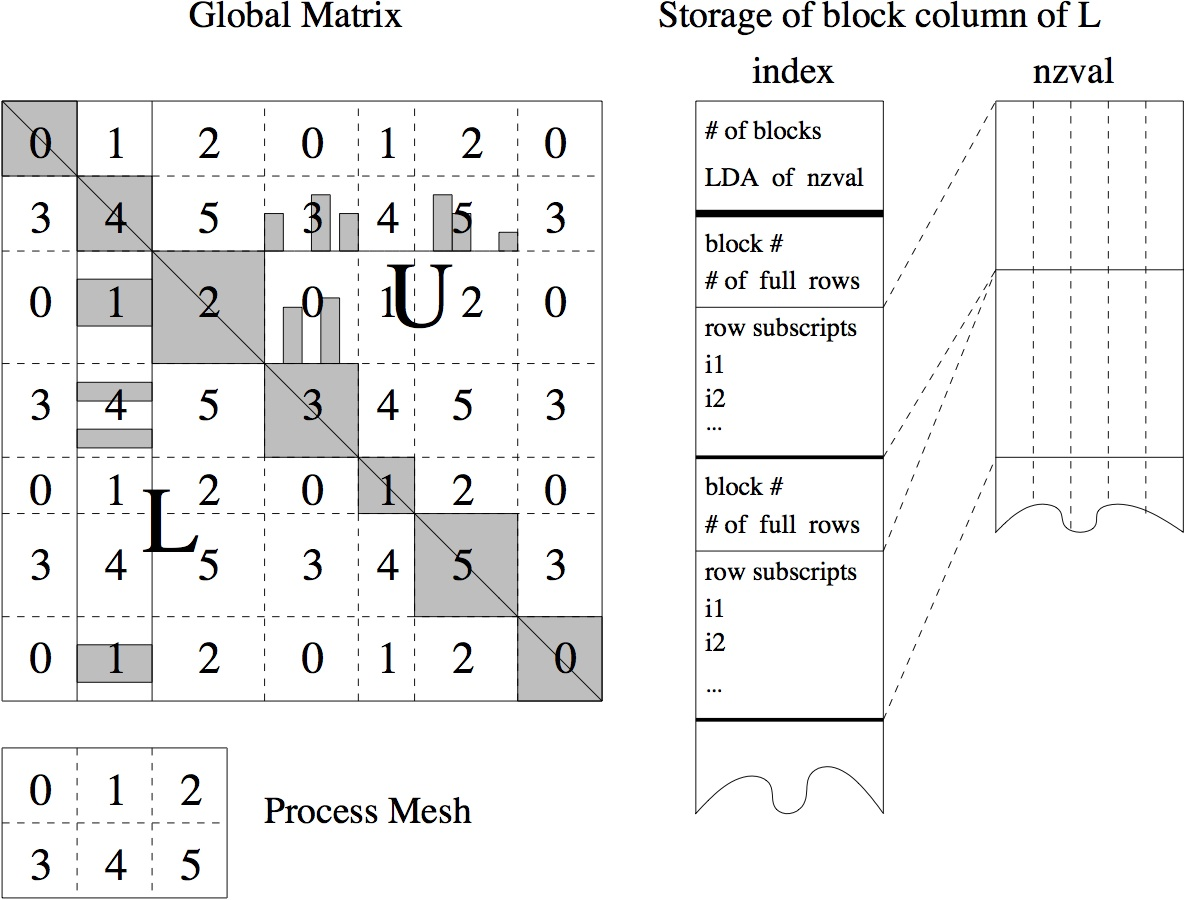
\includegraphics[width=0.6\textwidth]{lu_2d.jpg} }%
%\vspace{-5mm}
\caption{The 2 block-cyclic layout and the data structure
	to store a local block column of $L$.}
\label{fig:lu_2d}
\end{figure}


\section{Process grid and MPI communicator}
\label{sec:grid}
All MPI applications begin with a default communication domain
that includes all processes, say $N_p$, of this parallel job.
The default communicator {\tt MPI\_COMM\_WORLD} represents
this communication domain.
The $N_p$ processes are identified as a linear array of process IDs in the
range $0\;\ldots\;N_p-1$.

\subsection{2D process grid}
For {\superlud} library, we create a new process group derived from an
existing group using $N_g$ processes. There is a good
reason to use a new group rather than {\tt MPI\_COMM\_WORLD}, that is,
the message passing calls of the SuperLU library will be isolated
from those in other libraries or in the user's code.
For better scalability of the $LU$ factorization, we map the
1D array of $N_g$ processes into a logical 2D process grid.
This grid will have {\tt nprow} process rows and {\tt npcol} process columns,
such that ${\tt nprow} * {\tt npcol} = N_g$. A process can be referenced
either by its rank in the new group or by its coordinates within
the grid.
The routine {\tt superlu\_gridinit} maps already-existing processes
to a 2D process grid.
% A typical code fragment to accomplish this task would be the following:

\begin{verbatim}
    superlu_gridinit(MPI_Comm Bcomm, int nprow, int npcol, gridinfo_t *grid);
\end{verbatim}

%{\em Note that the underlined arguments in the calling sequence
%denote output arguments.}
This process grid will use the first ${\tt nprow} * {\tt npcol}$
processes from the base MPI communicator {\tt Bcomm}, and assign them
to the grid in a row-major ordering.
The input argument {\tt Bcomm} is an MPI communicator
representing the existing base group upon which the new
group will be formed. For example, it can be
{\tt MPI\_COMM\_WORLD}. The output argument {\tt grid}
represents the derived group to be used in {\superlud}.
{\tt Grid} is a structure containing the following fields:
\begin{verbatim}
   struct {
       MPI_Comm comm;        /* MPI communicator for this group */
       int iam;              /* my process rank in this group   */
       int nprow;            /* number of process rows          */
       int npcol;            /* number of process columns       */
       superlu_scope_t rscp; /* process row scope               */
       superlu_scope_t cscp; /* process column scope            */
   } grid;
\end{verbatim}

In the $LU$ factorization, some communications occur only among
the processes in a row (column), not among all processes.
For this purpose, we introduce two process subgroups,
namely {\tt rscp} (row scope) and {\tt cscp} (column scope).
For {\tt rscp} ({\tt cscp}) subgroup,
all processes in a row (column) participate in the communication.

The macros {\tt MYROW(iam, grid)} and {\tt MYCOL(iam, grid)} give
the row and column coordinates in the 2D grid of the process 
who has rank {\tt iam}.

\paragraph\
{\em NOTE: All processes in the base group, including those not in the
new group, must call this grid creation routine. This is required by
the MPI routine {\tt MPI\_Comm\_create} to create a new communicator.}


\subsection{Arbitrary grouping of processes}
It is sometimes desirable to divide up the processes into several subgroups,
each of which performs independent work of a single application.
In this situation, we cannot simply use the first ${\tt nprow} * {\tt npcol}$
processes to define the grid.
A more sophisticated process-to-grid mapping routine
{\tt superlu\_gridmap} is designed to create a grid with
processes of arbitrary ranks.
% A typical code fragment would be the following:

\begin{verbatim}
    superlu_gridmap(MPI_Comm Bcomm, int nprow, int npcol,
                    int usermap[], int ldumap, gridinfo_t *grid);
\end{verbatim}

The array {\tt usermap[]} contains the processes to be used
in the newly created grid. {\tt usermap[]} is indexed like a
Fortran-style 2D array with {\tt ldumap} as the leading dimension.
So {\tt usermap[i+j$*$ldumap]} (i.e., {\tt usermap(i,j)} in
Fortran notation) holds the process rank
to be placed in \{i, j\} position of the 2D process grid.
After grid creation, this subset of processes is logically numbered
in a consistent manner with the initial set of processes; that is,
they have the ranks in the range $0\;\ldots\;{\tt nprow} * {\tt npcol}-1$
in the new grid.
For example, if we want to map 6 processes with ranks $11\;\ldots\;16$
into a $2\times 3$ grid, we define
${\tt usermap} = \{11, 14, 12, 15, 13, 16\}$ and ${\tt ldumap}=2$.
Such a mapping is shown below
\begin{center}
\begin{tabular}{c|c|c|c|}
\multicolumn{1}{c}{} &\multicolumn{1}{c}{0}
  &\multicolumn{1}{c}{1}
  &\multicolumn{1}{c}{2}\\\cline{2-4}
0 &11 &12 &13 \\\cline{2-4}
1 &14 &15 &16 \\\cline{2-4}
\end{tabular}
\end{center}

\paragraph\
{\em NOTE: All processes in the base group, including those not in
the new group, must call this routine.}

{\tt Superlu\_gridinit} simply calls {\tt superlu\_gridmap}
with {\tt usermap[]} holding the first ${\tt nprow} * {\tt npcol}$
process ranks.

%%%%%%%%%%%%%%%%%%%%%%%%%%%%%%%%%%%%%%%%%%%%%%%%%%%%%%%%%%%%%%%%%%%%%%%
\section{Algorithmic background}
Although partial pivoting is used in both sequential and shared-memory
parallel factorization algorithms, it is not used in the
distributed-memory parallel algorithm, because it requires dynamic adaptation
of data structures and load balancing, and so is hard to make it scalable.
We use alternative techniques to stabilize the algorithm, which include
statically pivot large elements to the diagonal, single-precision
diagonal adjustment to avoid small pivots, and iterative refinement.
Figure~\ref{fig:GESP_alg} sketches our GESP algorithm
(Gaussian elimination with Static Pivoting).
Numerical experiments show that for a wide range of problems,
GESP is as stable as GEPP~\cite{lidemmel03}.

\begin{figure}[htbp]
\begin{tabbing}
jnk \= jnk \= jnk \= jnk \= jnk \= jnk \= xxxxx \= xxxxxxxxxxxxxxx \kill
\>(1) Perform row/column equilibration and row permutation:
	$A \leftarrow P_r\cdot D_r\cdot A\cdot D_c$, \\
\> \>	where $D_r$ and $D_c$ are diagonal matrices and $P_r$ is a row 
        permutation chosen \\
\> \>	to make the diagonal large compared to the off-diagonal.\\
\>(2) Find a column permutation $P_c$ to preserve sparsity:
	$A\leftarrow P_c\cdot A\cdot P_c^T$ \\
\>(3) Perform symbolic analysis to determine the nonzero structures of $L$ and $U$.\\
\>(4) Factorize $A=L\cdot U$ with control of diagonal magnitude: \\
\>\>\> {\bf if} ( $|a_{ii}| < \sqrt{\varepsilon}\cdot \|A\|_1$ ) {\bf then} \\
\>\>\>\> set $a_{ii}$ to $\sqrt{\varepsilon}\cdot \|A\|_1$\\
\>\>\> {\bf endif} \\
\>(5) Perform triangular solutions using $L$ and $U$.\\
\>(6) If needed, use an iterative solver like GMRES or iterative refinement (shown below) \\
\>\>\>{\bf iterate}:\\
\>\>\>\>$r = b - A\cdot x$  \hspace{0.98in} $\ldots$ sparse matrix-vector 
multiply \\
\>\>\>\>Solve $A\cdot dx = r$     \hspace{.77in} $\ldots$ triangular solution\\
\>\>\>\>$berr = \max_i\frac{|r|_i}{(|A|\cdot|x|+|b|)_i}$
                    \hspace{.3in} $\ldots$ componentwise backward error \\
\>\>\>\>{\bf if} ( $berr > \varepsilon$ and 
		   $berr \le \frac{1}{2}\cdot lastberr$ )
%\>\>\>\>{\bf if} ( $\frac{\|dx\|}{\|x\|} > \varepsilon$ 
%		   and $\frac{\|r\|}{\|A\|_1\cdot\|x\|} > \varepsilon$ )
%		   and $\|dx\| < last\_d$ )
	{\bf then} \\
\>\>\>\>\> $x = x + dx$   \\
\>\>\>\>\> $lastberr = berr$\\
\>\>\>\>\>{\bf goto iterate} \\
\>\>\>\>{\bf endif} \\
\>(7) If desired, estimate the condition number of $A$
\end{tabbing}
\caption{The outline of the GESP algorithm.}
\label{fig:GESP_alg}
\end{figure}

\ignore{ %%%%%%%%%%%%%%%%%%%%
\begin{figure}
\begin{tabbing}
jnk \= jnk \= jnk \= jnk \= jnk \= jnk \= xxxxx \= xxxxxxxxxxxxxxx \kill
\>(1) Row/column equilibration: $A \leftarrow D_r\cdot A\cdot D_c$ \\
\> \>	$D_r$ and $D_c$ are diagonal matrices chosen so that the
	largest entry of each row and \\
\> \>   column is $\pm 1$. \\
\>(2) Row permutation:  $A \leftarrow P_r \cdot A$ \\
\> \>	$P_r$ is a row permutation chosen to make the diagonal large
	compared to the off-diagonal.\\
% \>(2) Find a row permutation $P_r$ to put large entries on the diagonal:
% 	 $A\leftarrow P_r\cdot  A$ \\
%\>\>\>{\bf if} ( there are zeros on diagonal of $A$ ) {\bf then} \\
%\>\>\>\>1) drop $a_{ij}$ if $|a_{ij}| < \eta\cdot ||A||$
%	\ \ ( $\eta = 10^{-7}, 10^{-5}, ..., 10^{-1}$ ) \\
%\>\>\>\>2) apply maximum bipartite matching to the new $A$ \\
%\>\>\>{\bf endif} \\
\>(3) Find a column permutation $P_c$ to preserve sparsity:
	$A\leftarrow P_c\cdot A\cdot P_c^T$ \\
\>(4) Factorize $A=L\cdot U$ with control of diagonal magnitude \\
\>\>\> {\bf if} ( $|a_{ii}| < \sqrt{\varepsilon}\cdot ||A||$ ) {\bf then} \\
\>\>\>\> set $a_{ii}$ to $\sqrt{\varepsilon}\cdot ||A||$\\
\>\>\> {\bf endif} \\
\>(5) Solve $A\cdot x=b$ using the $L$ and $U$ factors, with the following
	iterative refinement \\
\>\>\>{\bf iterate}:\\
\>\>\>\>$r = b - A\cdot x$  \hspace{1in} $\ldots$ sparse matrix-vector 
multiply \\
\>\>\>\>Solve $A\cdot dx = r$     \hspace{.78in} $\ldots$ triangular solution\\
\>\>\>\>$berr = \max_i\frac{|r|_i}{(|A|\cdot|x|+|b|)_i}$
                    \hspace{.3in} $\ldots$ componentwise backward error \\
\>\>\>\>{\bf if} ( $berr > \varepsilon$ and 
		   $berr \le \frac{1}{2}\cdot lastberr$ )
%\>\>\>\>{\bf if} ( $\frac{||dx||}{||x||} > \varepsilon$ 
%		   and $\frac{||r||}{||A||\cdot||x||} > \varepsilon$ )
%		   and $||dx|| < last\_d$ )
	{\bf then} \\
\>\>\>\>\>$x = x + dx$   \\
 \>\>\>\>\>$lastberr = berr$\\
\>\>\>\>\>{\bf goto iterate} \\
\>\>\>\>{\bf endif} \\
\end{tabbing}
\vspace*{-.3in}
\caption{The outline of the GESP algorithm.}
\label{fig:GESP_alg}
\end{figure}
} %%%% ignore

Step (1) is accomplished by a weighted bipartite matching algorithm
due to Duff and Koster~\cite{duffkoster99}. Currently, process 0
computes $P_r$ and then broadcasts it to all the other processes.
If the distributed input interface is used (Section~\ref{sec:DistInput}),
we first gather the distributed matrix $A$  onto processor 0.
Work is underway to remove this sequential bottleneck.

In Step (2), we provide several ordering options, such as 
multiple minimum degree ordering~\cite{liu85} on the graphs of 
$A+A^T$, or the {\metis}~\cite{kaku:98a} ordering on the graphs of $A+A^T$.
% and the approximate minimum degree column ordering~\cite{davisgilbert00}.
The user can use any other ordering in place of the ones provided
in the library.
({\em Note, since we will pivot on the diagonal in step (4),
an ordering based on the structure of $A+A^T$ almost always yields sparser
factors than that based on the structure of $A^TA$.
This is different from SuperLU and SuperLU\_MT, where we allow to pivot
off-diagonal.})
In this step, when a sequential ordering algorithm is used, every process
runs the same algorithm independently.

Step (3) can be done either sequentially or in parallel
depending on how the \textsf{options} argument is set
(see Section~\ref{sec:drivers} for details.)
The parallel symbolic factorization was a newly added feature
since the \textsf{v2.1} release. 
It is designed tightly around the separator tree returned from
a graph partitioning type of ordering (presently we use
{\parmetis}~\cite{kaku:03}), and works only on power-of-two
processors.  We first re-distribute the graph of $A$
onto the largest $2^q$ number of processors
which is smaller than the total $N_p$ processors, then perform
parallel symbolic factorization, and finally re-populate the
$\{L \backslash U\}$ structure to all $N_p$ processors.
The algorithm and performance was studied in~\cite{grigoridemmelli07}.
To invoke parallel symbolic factorization, the user needs to set
the two fields of the \textsf{options} argument as follows:
\begin{verbatim}
    options.ParSymbFact       = YES
    options.ColPerm           = PARMETIS;
\end{verbatim}
Note that, even if the user sets \textsf{options.ColPerm} to use an ordering
algorithm other than {\parmetis}, the driver routine overrides it with
{\parmetis} when it sees \textsf{options.ParSymbFact = YES}.

Steps (4) to (7) are the most time-consuming steps and were parallelized
a while ago, see the papers~\cite{lidemmel03,li05}.


\subsection{Multicore and GPU enhancements}
Given that the node architecture trend is to have many simpler cores
on a NUMA node, possibly with GPU-like accelerators, and the
amount of memory per-core becomes smaller, the pure MPI model
does not match the light-weight processor architecture.
We need to resort to other forms of parallelism
at node level. In sparse factorization (step (4) in Figure~\ref{fig:GESP_alg}),
the Schur complement update after each panel factorization step exhibits
ample fine-grid parallelism. We have designed the OpenMP + CUDA
code to exploit the on-node parallelism. For each MPI task of the 
Schur complement update, we aggegrate the small $L$ and $U$ matrix blocks
into a larger block, divide the GEMM work between CPU and GPU using
some heuristic performance model, offload the larger block of GEMM
to GPU.  The key to success is to overlap the CPU work 
(multithreaded Scatter/Gather, some portion of GEMM) with
the GPU work (GEMM with multiple CUDA streams). This way, we are able
to hide the latency time due to PCI bus transfer between CPU and GPU.
The detailed algorithm description and performance data were given
in the paper by Sao et al.~\cite{sao2014}.

To use Nvidia GPU, you must set the following
Linux shell environment variable before compilation:

\vspace{.1in}
{\tt setenv ACC GPU}
\vspace{.1in}

Hybrid MPI+OpenMP setting may outperform MPI-only configurations in some
cases and in most cases hybrid MPI+OpenMP would require less memory.
The environment variable {\tt OMP\_NUM\_THREADS} needs to be set appropriately.
Hybrid configuration obtains threaded parallelism from both,
explicit OpenMP pragmas and multithreaded BLAS. Thus for good performance
it is better if OpenMP threading library and BLAS threading are synergistic.
For example, when using Intel MKL libray, just setting {\tt OMP\_NUM\_THREADS}
would set the number of threads for both MKL and OpenMP. However,
it is possible to have different number of threads for MKL, in which case
{\tt MKL\_NUM\_THREADS} controls the number of threads used by MKL. 
In our case, just setting {\tt OMP\_NUM\_THREADS} is sufficient. 

Triangular solve phase does not use multithreading yet.
The MPI-only configuration may be more suitable in case of
many right hand sides or in other cases, where solve phase seems
to be a performance bottleneck.


\section{{\tt Options} argument}
\label{sec:options}
One important input argument is {\tt options}, which controls how the
linear system will be solved.
Although the algorithm presented in~\fig{GESP_alg} consists of
seven steps, for some matrices not all steps are needed to get
accurate solution. For example, for diagonally dominant matrices, 
choosing the diagonal pivots ensures the stability;
there is no need for row pivoting in step (1).
In another situation where a sequence of matrices with the
same sparsity pattern need be factorized, the column
permutation $P_c$ (and also the row permutation $P_r$, if
the numerical values are similar) need be computed only
once, and reused thereafter. ($P_r$ and $P_c$
are implemented as permutation vectors {\tt perm\_r} and {\tt perm\_c}.)
For the above examples, performing all seven steps does more
work than necessary. 
{\tt Options} is used to accommodate the various requirements of applications;
it contains the following fields:
\begin{itemize}
\item {\tt Fact}\\
    Specifies whether or not the factored form of the matrix
    $A$ is supplied on entry, and if not, how the matrix $A$ will
    be factored base on some assumptions of the previous history.
    {\tt fact} can be one of:
    \begin{itemize}
    \item {\tt DOFACT}: the matrix $A$ will be factorized from scratch.
    \item {\tt SamePattern}: the matrix $A$ will be factorized assuming
	that a factorization of a matrix with the same sparsity pattern
	was performed prior to this one. Therefore, this factorization
        will reuse column permutation vector {\tt perm\_c}.
    \item {\tt SampPattern\_SameRowPerm}: the matrix $A$ will be factorized
	assuming that a factorization of a matrix with the same sparsity
	pattern and similar numerical values was performed prior to this one.
        Therefore, this factorization will reuse both row and column
        permutation vectors {\tt perm\_r} and {\tt perm\_c}, both row and
	column scaling factors $D_r$ and $D_c$, and the distributed data
	structure set up from the previous symbolic factorization.
    \item {\tt FACTORED}: the factored form of $A$ is input.
    \end{itemize}
\item {\tt Equil}  \{ {\tt YES} $|$ {\tt NO} \} \\
    Specifies whether to equilibrate the system.
\item {\tt ParSymbFact}   \{ {\tt YES} $|$ {\tt NO} \} \\ 
    Specifies whether to perform parallel symbolic factorization.
    If it is set to \textsf{YES}, the \textsf{ColPerm} field should
    be set to \textsf{PARMETIS}. Otherwise, the driver routine {\tt pdgssvx}
    will use {\parmetis} anyway, ignoring the other setting in
    \textsf{ColPerm}.
\item {\tt ColPerm}\\
    Specifies the column ordering method for fill reduction.
    \begin{itemize}
    \item {\tt NATURAL}: natural ordering.
    \item {\tt MMD\_AT\_PLUS\_A}: minimum degree ordering on the
			structure of $A^T+A$.
    \item {\tt MMD\_ATA}: minimum degree ordering on the structure of
			$A^TA$.
    \item {\tt METIS\_AT\_PLUS\_A}: {\metis} ordering on the
			structure of $A^T+A$.
    \item {\tt PARMETIS}: {\parmetis} ordering on the structure of $A^T+A$.
%            This can only be used with parallel symbolic factorization
%            (i.e., {\tt ParSymbFact = YES}).
    \item {\tt MY\_PERMC}: use the ordering given in {\tt perm\_c} input by
	                the user.
    \end{itemize}
\item {\tt RowPerm} \\
    Specifies how to permute rows of the original matrix.
    \begin{itemize}
    \item {\tt NATURAL}: use the natural ordering.
    \item {\tt LargeDiag\_MC64}: use a serial, weighted bipartite matching
      algorithm implemented in MC64 to permute the rows to make the
      diagonal large relative to the off-diagonal~\cite{duffkoster01}.
    \item {\tt LargeDiag\_AWPM}: use a parallel, approximate weighted bipartite
      matching algorithm implemented in CombBLAS to permute the rows to
      make the diagonal large relative to the off-diagonal~\cite{awpm}.
    \item {\tt MY\_PERMR}: use the ordering given in {\tt perm\_r} input by the user.
    \end{itemize}
\item {\tt ReplaceTinyPivot} \{ {\tt YES} $|$ {\tt NO} \} \\ 
    Specifies whether to replace the tiny diagonals by
           $\sqrt\varepsilon\cdot||A||$ during $LU$ factorization.
\item {\tt IterRefine}\\
    Specifies how to perform iterative refinement.
    \begin{itemize}
    \item {\tt NO}: no iterative refinement.
    \item {\tt DOUBLE}: accumulate residual in double precision.
    \item {\tt EXTRA}:  accumulate residual in extra precision.
	 ({\em not yet implemented.})
    \end{itemize}
\item {\tt Trans}  \{ {\tt NOTRANS} $|$ {\tt TRANS} $|$ {\tt CONJ} \} \\
    Specifies whether to solve the transposed system.
\item {\tt SolveInitialized}  \{ {\tt YES} $|$ {\tt NO} \} \\
    Specifies whether the initialization has been performed to
    the triangular solve. \\
   (used only by the distributed input interface)
\item {\tt RefineInitialized}  \{ {\tt YES} $|$ {\tt NO} \} \\
    Specifies whether the initialization has been performed to
    the sparse matrix-vector multiplication routine needed in the
    iterative refinement. \\
    (used only by the distributed input interface)
\item {\tt num\_lookaheads}  \{ integer \} \\
    Specifies the number of levels in the look-ahead factorization
\item {\tt lookahead\_etree}  \{ {\tt YES} $|$ {\tt NO} \} \\
    Specifies whether to use the elimination tree computed from the 
    serial symbolic factorization to perform static scheduling.
\item {\tt SymPattern}  \{ {\tt YES} $|$ {\tt NO} \} \\
    Gives the scheduling algorithm a hint whether the matrix
    has the symmetric pattern.
 \item {\tt PrintStat}  \{ {\tt YES} $|$ {\tt NO} \} \\
    Specifies whether to print the solver's statistics.
\end{itemize}

There is a routine named {\tt set\_default\_options\_dist()} that sets the
default values of these options, which are:
\begin{verbatim}
    fact              = DOFACT           /* factor from scratch */
    equil             = YES
    ParSymbFact       = NO
    colperm           = MMD_AT_PLUS_A
    rowperm           = LargeDiag        /* use MC64 */
    ReplaceTinyPivot  = YES
    IterRefine        = DOUBLE
    Trans             = NOTRANS
    SolveInitialized  = NO
    RefineInitialized = NO
    num_lookaheads    = 10;
    lookahead_etree   = NO;
    SymPattern        = NO;
    PrintStat         = YES
\end{verbatim}


\section{Basic steps to solve a linear system}
In this section, we use a complete sample program to illustrate
the basic steps required to use {\superlud}.
This program is listed below, and is also available
as {\tt EXAMPLE/pddrive.c} in the source code distribution.
All the routines must include the header file {\tt superlu\_ddefs.h}
(or {\tt superlu\_zdefs.h}, the complex counterpart)
which contains the definitions of the data types, the macros and
the function prototypes.

\begin{verbatim}
#include <math.h>
#include "superlu_ddefs.h"

main(int argc, char *argv[])
/*
 * Purpose
 * =======
 *
 * The driver program PDDRIVE.
 *
 * This example illustrates how to use PDGSSVX with the full
 * (default) options to solve a linear system.
 * 
 * Five basic steps are required:
 *   1. Initialize the MPI environment and the SuperLU process grid
 *   2. Set up the input matrix and the right-hand side
 *   3. Set the options argument
 *   4. Call pdgssvx
 *   5. Release the process grid and terminate the MPI environment
 *
 * On the Cray T3E, the program may be run by typing
 *    mpprun -n <procs> pddrive -r <proc rows> -c <proc columns> <input_file>
 *
 */
{
    superlu_options_t options;
    SuperLUStat_t stat;
    SuperMatrix A;
    ScalePermstruct_t ScalePermstruct;
    LUstruct_t LUstruct;
    SOLVEstruct_t SOLVEstruct;
    gridinfo_t grid;
    double   *berr;
    double   *b, *xtrue;
    int_t    m, n, nnz;
    int_t    nprow, npcol;
    int      iam, info, ldb, ldx, nrhs;
    char     trans[1];
    char     **cpp, c;
    FILE *fp, *fopen();

    nprow = 1;  /* Default process rows.      */
    npcol = 1;  /* Default process columns.   */
    nrhs = 1;   /* Number of right-hand side. */

    /* ------------------------------------------------------------
       INITIALIZE MPI ENVIRONMENT. 
       ------------------------------------------------------------*/
    MPI_Init( &argc, &argv );

    /* Parse command line argv[]. */
    for (cpp = argv+1; *cpp; ++cpp) {
        if ( **cpp == '-' ) {
            c = *(*cpp+1);
            ++cpp;
            switch (c) {
              case 'h':
                  printf("Options:\n");
                  printf("\t-r <int>: process rows    (default %d)\n", nprow);
                  printf("\t-c <int>: process columns (default %d)\n", npcol);
                  exit(0);
                  break;
              case 'r': nprow = atoi(*cpp);
                  break;
              case 'c': npcol = atoi(*cpp);
                  break;
            }
        } else { /* Last arg is considered a filename */
            if ( !(fp = fopen(*cpp, "r")) ) {
                ABORT("File does not exist");
            }
            break;
        }
    }

    /* ------------------------------------------------------------
       INITIALIZE THE SUPERLU PROCESS GRID. 
       ------------------------------------------------------------*/
    superlu_gridinit(MPI_COMM_WORLD, nprow, npcol, &grid);

    /* Bail out if I do not belong in the grid. */
    iam = grid.iam;
    if ( iam >= nprow * npcol )	goto out;

    /* ------------------------------------------------------------
       GET THE MATRIX FROM FILE AND SETUP THE RIGHT HAND SIDE. 
       ------------------------------------------------------------*/
    dcreate_matrix(&A, nrhs, &b, &ldb, &xtrue, &ldx, fp, &grid);

    if ( !(berr = doubleMalloc_dist(nrhs)) )
        ABORT("Malloc fails for berr[].");

    /* ------------------------------------------------------------
       NOW WE SOLVE THE LINEAR SYSTEM.
       ------------------------------------------------------------*/

    /* Set the default input options. */
    set_default_options_dist(&options);

    m = A.nrow;
    n = A.ncol;

    /* Initialize ScalePermstruct and LUstruct. */
    ScalePermstructInit(m, n, &ScalePermstruct);
    LUstructInit(n, &LUstruct);

    /* Initialize the statistics variables. */
    PStatInit(&stat);

    /* Call the linear equation solver. */
    pdgssvx(&options, &A, &ScalePermstruct, b, ldb, nrhs, &grid,
            &LUstruct, &SOLVEstruct, berr, &stat, &info);


    /* Check the accuracy of the solution. */
    pdinf_norm_error(iam, ((NRformat_loc *)A.Store)->m_loc,
                     nrhs, b, ldb, xtrue, ldx, &grid);

    PStatPrint(&options, &stat, &grid);        /* Print the statistics. */

    /* ------------------------------------------------------------
       DEALLOCATE STORAGE.
       ------------------------------------------------------------*/

    PStatFree(&stat);
    Destroy_CompRowLoc_Matrix_dist(&A);
    ScalePermstructFree(&ScalePermstruct);
    Destroy_LU(n, &grid, &LUstruct);
    LUstructFree(&LUstruct);
    if ( options.SolveInitialized ) {
        dSolveFinalize(&options, &SOLVEstruct);
    }
    SUPERLU_FREE(b);
    SUPERLU_FREE(xtrue);
    SUPERLU_FREE(berr);

    /* ------------------------------------------------------------
       RELEASE THE SUPERLU PROCESS GRID.
       ------------------------------------------------------------*/
out:
    superlu_gridexit(&grid);

    /* ------------------------------------------------------------
       TERMINATES THE MPI EXECUTION ENVIRONMENT.
       ------------------------------------------------------------*/
    MPI_Finalize();

}
\end{verbatim}

Five basic steps are required to call a SuperLU routine:
\begin{enumerate}
\item Initialize the MPI environment and the SuperLU process grid.\\
	This is achieved by the calls to the MPI routine {\tt MPI\_Init()}
	and the SuperLU routine\\ {\tt superlu\_gridinit()}.
	In this example, the communication domain for SuperLU is built upon
	the MPI default communicator {\tt MPI\_COMM\_WORLD}.
	In general, it can be built upon any MPI communicator.
	\Cref{sec:grid} contains the details about this step.
\item Set up the input matrix and the right-hand side.\\
        This example uses the interface with the distributed input matrices,
        see Section~\ref{sec:DistInput}.
        In most practical applications, the matrices can be
        generated on each process without the need to have a centralized
        place to hold them.
        But for this example, we let process 0 read the input matrix stored
        on disk	in Harwell-Boeing format~\cite{duffgrimes92}
        (a.k.a. compressed column storage), and distribute it to all the
        other processes, so that each process only owns a block of rows of
        matrix. The right-hand side matrix is generated
	so that the exact solution matrix consists of all ones.
        The subroutine {\tt dcreate\_matrix()} accomplishes this task.
\item Initialize the input arguments: {\tt options, ScalePermstruct, LUstruct,
        stat}.\\
        The input argument {\tt options} controls how the linear system would
  	be solved---use equilibration or not, how to order the rows and
	the columns of the matrix, use iterative refinement or not.
	The subroutine {\tt set\_default\_options\_dist()} sets the
        {\tt options} argument so that the solver performs all the
        functionality. You can also set it up according to your own needs,
        see section~\ref{sec:options} for the fields of this structure.
        {\tt ScalePermstruct} is the data structure that stores 
	the several vectors describing the transformations
        done to $A$. {\tt LUstruct} is the data structure
        in which the distributed $L$ and $U$ factors are stored.
	{\tt Stat} is a structure collecting the statistics about
	runtime and flop count, etc.
\item Call the SuperLU routine {\tt pdgssvx()}.
\item Release the process grid and terminate the MPI environment.\\
	After the computation on a process grid has been completed, the
	process grid should be released by a call to the SuperLU routine
	{\tt superlu\_gridexit()}.
        When all computations have been completed, the MPI routine
        {\tt MPI\_Finalize()} should be called.
\end{enumerate}


\section{User-callable routines}
%% Appendix~\ref{chap:superlu_dist_spec} contains the complete specifications
%% of the routines in SuperLU\_DIST.

\subsection{Driver routines}
\label{sec:drivers}
There are two driver routines to solve systems of linear equations,
which are named {\tt pdgssvx\_ABglobal} for the global input interface,
and {\tt pdgssvx} for the distributed interface.
We recommend that the general users, especially the beginners, 
use a driver routine rather than the computational
routines, because correctly using the driver routine does not require
thorough understanding of the underlying data structures.
Although the interface of these routines are simple, we expect their rich 
functionality can meet the requirements of most applications.
{\tt Pdgssvx\_ABglobal}/{\tt pdgssvx} perform the following functions:
\begin{itemize}
\item Equilibrate the system (scale $A$'s rows and columns to
	have unit norm) if $A$ is poorly scaled;
\item Find a row permutation that makes diagonal of $A$ large
	relative to the off-diagonal;
\item Find a column permutation that preserves the sparsity of
	the $L$ and $U$ factors;
\item Solve the system $AX=B$ for $X$ by factoring $A$
	followed by forward and back substitutions;
\item Refine the solution $X$.
\end{itemize}


\subsection{Computational routines}
The experienced users can invoke the following computational routines
to directly control the behavior of {\superlud} in order to meet their
requirements.
\begin{itemize}
\item {\tt pdgstrf()}: Factorize in parallel. \\
	This routine factorizes the input matrix $A$ (or the scaled and
	permuted $A$). It assumes that the distributed data structures
	for $L$ and $U$ factors are already set up, and the initial
  	values of $A$ are loaded into the data structures.
	If not, the routine {\tt symbfact()} should be called to
	determine the nonzero patterns of the factors, and the
	routine {\tt pddistribute()} should be called to distribute the matrix.
	{\tt Pdgstrf()} can factor non-square matrices.
%	Currently, $A$ must be globally available on all processes.
\item {\tt pdgstrs()/pdgstrs\_Bglobal()}: Triangular solve in parallel. \\
	This routine solves the system by forward and back
	substitutions using the the $L$ and $U$ factors
	computed by {\tt pdgstrf()}. {\tt Pdgstrs()} takes distributed $B$.
	For {\tt pdgstrs\_Bglobal()}, $B$ must be globally available on
        all processes. 
\item {\tt pdgsrfs()/pdgsrfs\_ABXglobal()}: Refine solution in parallel. \\
	Given $A$, its factors $L$ and $U$, and an initial solution
	$X$, this routine performs iterative refinement.
	{\tt Pdgsrfs()} takes distributed $A$, $B$ and $X$.
	For {\tt pdgsrfs\_ABXglobal()}, $A$, $B$ and $X$ must be globally
        available on all processes. 
\end{itemize}

\subsection{Utility routines}
\label{sec:slud_utility}

The following utility routines can help users create and destroy the
{\superlud} matrices. These routines reside in three places: {\tt SRC/util.c},
{\tt SRC/\{d,z\}util.c}, and {\tt SRC/p\{d,z\}util.c}.
Most of the utility routines in sequential {\superlu} can also be used
in {\superlud} for the local data, see Section~\ref{sec:slu_utility}.
Here, we only list those new routines
specific to {\superlud}. Note that in order to avoid name clash between
{\superlu} and {\superlud}, we append ``{\tt \_dist}'' to each routine
name in {\superlud}.

\begin{verbatim}
    /* Create a supermatrix in distributed compressed row format. A is output. */
    dCreate_CompRowLoc_Matrix_dist(SuperMatrix *A, int_t m, int_t n,
                                   int_t nnz_loc, int_t m_loc, int_t fst_row,
                                   double *nzval, int_t *colind, int_t *rowptr,
                                   Stype_t stype, Dtype_t dtype, Mtype_t mtype);

    /* Deallocate the supermatrix in distributed compressed row format. */
    Destroy_CompRowLoc_Matrix_dist(SuperMatrix *A);

    /* Allocate storage in ScalePermstruct. */
    ScalePermstructInit(const int_t m, const int_t n,
                        ScalePermstruct_t *ScalePermstruct);

    /* Deallocate ScalePermstruct */
    ScalePermstructFree(ScalePermstruct_t *ScalePermstruct);

    /* Allocate storage in LUstruct. */
    LUstructInit(const int_t n, LUstruct_t *LUstruct);

    /* Deallocate the distributed L & U factors in LUstruct. */
    Destroy_LU(int_t n, gridinfo_t *grid, LUstruct_t *LUstruct);

    /* Deallocate LUstruct. */
    LUstructFree(LUstruct_t *LUstruct);

    /* Initialize the statistics variable. */
    PStatInit(SuperLUStat_t *stat);

    /* Print the statistics. */
    PStatPrint(superlu_options_t *options, SuperLUStat_t *stat,
               gridinfo_t *grid);

    /* Deallocate the statistics variable. */
    PStatFree(SuperLUStat_t *stat);
\end{verbatim}


\section{Installation}
\label{sec:dist_install}
\subsection{File structure and complilation}
The top level SuperLU\_DIST/ directory is structured as follows:
\begin{verbatim}
    SuperLU_DIST/README.md instructions on installation
    SuperLU_DIST/CBLAS/    BLAS routines in C, functional but not fast
    SuperLU_DIST/DOC/      Users' Guide
    SuperLU_DIST/EXAMPLE/  example programs
    SuperLU_DIST/INSTALL/  test machine dependent parameters
    SuperLU_DIST/SRC/      C source code, to be compiled into libsuperlu_dist.a
    SuperLU_DIST/lib/      contains library archive libsuperlu_dist.a
    SuperLU_DIST/Makefile  top level Makefile that does installation and testing
    SuperLU_DIST/make.inc  compiler, compiler flags, library definitions and C
                           preprocessor definitions, included in all Makefiles.
                           (You may need to edit it to suit for your system
                            before compiling the whole package.)
    SuperLU_DIST/MAKE_INC/ sample machine-specific make.inc files
\end{verbatim}

You can use CMake automic build system to install the package. Please see
README.md for instruction. The following describes how to install manually
by editing a Makefile.

Before installing the package, you may need to edit
{\tt SuperLU\_DIST/make.inc} for your system.
This make include file is referenced inside all the Makefiles
in the various subdirectories. As a result, there is no need to 
edit the Makefiles in the subdirectories. All information that is
machine specific has been defined in this include file. 

Sample machine-specific {\tt make.inc} are provided in the
{\tt MAKE\_INC/} directory for several platforms, such as
Cray XE6 and IBM SP.
When you have selected the machine to which you wish to install
{\superlud}, you may copy the appropriate sample include file
(if one is present) into {\tt make.inc}. For example, if you wish to run
on a Cray XE6,  you can do:

\hspace{.4in}{\tt cp MAKE\_INC/make.xe6 make.inc}

For the systems other than those listed above, slight modifications to the
{\tt make.inc} file will need to be made.
In particular, the following items should be examined:
\begin{enumerate}   
\item The BLAS library.\\
   If there is a BLAS library available on your machine,
   you may define the following in {\tt make.inc}:

   \hspace{.4in}{\tt BLASDEF = -DUSE\_VENDOR\_BLAS}

   \vspace{-6pt}
   \hspace{.4in}{\tt BLASLIB = <BLAS library you wish to link with>}

   The {\tt CBLAS/} subdirectory contains the part of the BLAS (in C) needed by
   {\tt SuperLU\_DIST} package. However, these routines are intended for use
   only if there is no faster implementation of the BLAS already available
   on your machine. In this case, you should do the following:
   \begin{itemize}
   \item[1)]In make.inc, undefine (comment out) BLASDEF, define:

          \hspace{.4in}{\tt BLASLIB = ../lib/libblas\$(PLAT).a}

   \item[2)] At the top level SuperLU\_DIST directory, type:

          \hspace{.4in}{\tt make blaslib}

         to create the BLAS library from the routines in {\tt CBLAS/}
	 subdirectory.
   \end{itemize}

\item External libraries: {\metis} and {\parmetis}. \\
   If you will use {\metis} or {\parmetis} ordering, or parallel
   symbolic factorization (which depends on {\parmetis}), you will
   need to install them yourself. Since {\parmetis} package already
   contains the source code for the {\metis} library, you can just
   download {\parmetis} at:

   \hspace{.4in}\url{http://glaros.dtc.umn.edu/gkhome/metis/parmetis/download}

   After you have installed it, you should define the following in
   {\tt make.inc}:

   \hspace{.4in}{\tt PARMETIS\_DIR = <top-level {\parmetis} directory>}

   \vspace{-4pt}
   \hspace{.4in}{\tt METISLIB = -L\$(PARMETIS\_DIR)/build/Linux-x86\_64/libmetis -lmetis}

   \vspace{-4pt}
   \hspace{.4in}{\tt PARMETISLIB = -L\$(PARMETIS\_DIR)/build/Linux-x86\_64/libparmetis -lparmetis}

   \vspace{-4pt}
   \hspace{.4in}{\tt I\_PARMETIS = -I\$(PARMETIS\_DIR)/include -I\$(PARMETIS\_DIR)/metis/include}

\item C preprocessor definition {\tt CDEFS}.\\
   In the header file {\tt SRC/Cnames.h}, we use macros to determine how
   C routines should be named so that they are callable by Fortran.%
   \footnote{Some vendor-supplied BLAS libraries do not have C interfaces.
   So the re-naming is needed in order for the SuperLU BLAS calls (in C) to 
   interface with the Fortran-style BLAS.}
   The possible options for {\tt CDEFS} are:
   \begin{itemize}
   \item {\tt -DAdd\_}: Fortran expects a C routine to have an underscore
		        postfixed to the name;
   \item {\tt -DNoChange}: Fortran expects a C routine name to be identical to
		     that compiled by C;
   \item {\tt -DUpCase}: Fortran expects a C routine name to be all uppercase.
   \end{itemize}

\item (optional) Enable Nvidia GPU access.
   \begin{enumerate}
   \item Set the following Linux environment variable:
     {\tt setenv ACC GPU}
   \item Add the CUDA library location in {\tt make.inc}:
     \begin{verbatim}
    ifeq "${ACC}" "GPU"
    CFLAGS += -DGPU_ACC
    INCS += -I<CUDA directory>/include
    LIBS += -L<CUDA directory>/lib64 -lcublas -lcudart 
    endif
     \end{verbatim}
   \end{enumerate}
\end{enumerate}
   
A {\tt Makefile} is provided in each subdirectory. The installation can be
done automatically by simply typing ``{\tt make}'' at the top level.

Hybrid MPI+OpenMP setting is implemented in the factorization routines.
It may outperform MPI-only configurations in some cases and
requires less memory. 	To use OpenMP parallelism, you need to compile
the code with the following CPP definition:

\begin{verbatim}
  -D_OPENMP
\end{verbatim}
and set the number of threads to be used in the environment variable:
\begin{verbatim}
  setenv OMP_NUM_THREADS <##>
\end{verbatim}

\noindent needs to be set to enable this feature.

\subsection{Performance-tuning parameters}
\label{sec:SuperLU_DIST_sp_ienv}

Similar to sequential SuperLU, several performance related parameters
are set in the inquiry function {\tt sp\_ienv()}.
The declaration of this function is

\vspace{.1in}
{\tt int sp\_ienv(int ispec);}
\vspace{.1in}

{\tt Ispec} specifies the parameter to be returned%
\footnote{The numbering of 2, 3 and 6 is consistent with that used
in SuperLU and SuperLU\_MT.}:
\begin{tabbing}
xxxxxx \= xxxx \= junk \= \kill
\>ispec\>= 2: the relaxation parameter to control supernode amalgamation\\
\>     \>= 3: the maximum allowable size for a block (supernode) \\
\>     \>= 6: the estimated fills factor for the adjacency structures 
	      of $L$ and $U$
\end{tabbing}	    

The values to be returned may be set differently on different machines.
The setting of maximum block size (parameter 3) should take into
account the local Level 3 BLAS speed, the load balance and the 
degree of parallelism. Small block size may result in better
load balance and more parallelism, but poor individual node performance,
and vice versa for large block size. 

These parameters can also be set as Linux environment variables, so that the
routine {\tt sp\_ienv()} does not need to be recompiled every time when you
change the settings.

\begin{verbatim}
  setenv NREL <##>    /* parameter #2: maximum size of the relaxed supernode */
  setenv NSUP <##>    /* parameter #3: maximum supernode size */
\end{verbatim}

\noindent The following parameters are related to GPU usage:

\begin{verbatim}
  setenv CUBLAS_NB <##>        /* middle dimension of CUDA GEMM (default 64) */
  setenv MAX_BUFFER_SIZE <##>  /* maximum buffer size on GPU (default 5M words) */
\end{verbatim}

These parameters are described in detail in various algorithm
papers, see~\cite{li05,sao2014}.


\section{Example programs}
In the {\tt SuperLU\_DIST/EXAMPLE/} directory, we present a few sample
programs to illustrate the complete calling sequences to use the expert
driver to solve systems of equations.
These include how to set up the process grid and the input
matrix, how to obtain a fill-reducing ordering.
A {\tt Makefile} is provided to generate the executables.
A {\tt README} file in this directory shows how to run these examples.
The leading comment in each routine describes the functionality of
the example.
The two basic examples are {\tt pddrive\_ABglobal()} and {\tt pddrive()}.
The first shows how to use the global input interface, and the
second shows how to use the distributed input interface.


\section{Fortran 90 Interface}
\label{sec:slud_fortran}
We developed a complete Fortran 90 interface for {\superlud}.
All the interface files and an example driver program are located in the 
{\tt SuperLU\_DIST/FORTRAN/} directory. 
Table~\ref{tab:f90_files} lists all the files.

\begin{table}[hptb]
%%\centerline{
\small{
\begin{tabular}{ll}
f\_pddrive.f90          & An example Fortran driver routine. \\ \\
superlu\_mod.f90        & Fortran 90 module that defines the interface functions
                          to access {\superlud}'s \\
                        & data structures. \\ \\
superlupara.f90         & It contains parameters that correspond to
                          {\superlud}'s enums.\\ \\
hbcode1.f90             & Fortran function for reading a sparse Harwell-Boeing matrix from \\
                        & the file. \\  \\
superlu\_c2f\_wrap.c    & C wrapper functions, callable from Fortran.
                           The functions fall \\
                        & into three classes: 1) Those that allocate a
                           structure and return \\
                        & a handle, or deallocate the memory of a structure.
                          2) Those that \\
                        & get or set the value of a component of a struct.
                          3) Those that \\
                        & are wrappers for {\superlud} functions. \\ \\
dcreate\_dist\_matrix.c & C function for distributing the matrix in a distributed \\
                        & compressed row format.
% Note that here we adjust
%                          the $1$-based \\
%                        & indexing to $0$-based indexing which is required by
%                          the C routines.\\
\end{tabular}
}
\caption{The Fortran 90 interface files and an example driver routine.}
\label{tab:f90_files}
\end{table}

Note that in this interface, all objects (such as \textsf{grid},
\textsf{options}, etc.) in {\superlud} are \emph{opaque}, meaning their size
and structure are not visible to the Fortran user.
These opaque objects are allocated, deallocated and operated in the C side
and not directly accessible from Fortran side. They can only be accessed
via \emph{handles} that exist in Fortran's user space. In Fortran, all handles
have type \textsf{INTEGER}. Specifically, in our interface, the size of Fortran
handle is defined by \textsf{superlu\_ptr} in \textsf{superlupara.f90}.
For different systems, the size might need to be changed. Then using these
handles, Fortran user can call C wrapper routines to manipulate the opaque
objects. For example, you can call \textsf{f\_create\_gridinfo(grid\_handle)}
to allocate memory for structure \textsf{grid},
and return a handle \textsf{grid\_handle}.

% All callable interface (wrapper) routines are listed in Appendix.

The sample program illustrates the basic steps required to use {\superlud}
in Fortran to solve systems of equations. These include how to set up the
processor grid and the input matrix, how to call the linear equation solver.
This program is listed below, and is also available as \textsf{f\_pddrive.f90}
in the subdirectory. Note that the routine must include the moudle 
\textsf{superlu\_mod} which contains the definitions 
of all parameters and the Fortran wrapper functions. A \textsf{Makefile} is
provided to generate the executable. A \textsf{README} file in this
directory shows how to run the example. 

\begin{verbatim}
      program f_pddrive
! 
! Purpose
! =======
!
! The driver program F_PDDRIVE.
!
! This example illustrates how to use F_PDGSSVX with the full
! (default) options to solve a linear system.
! 
! Seven basic steps are required:
!   1. Create C structures used in SuperLU
!   2. Initialize the MPI environment and the SuperLU process grid
!   3. Set up the input matrix and the right-hand side
!   4. Set the options argument
!   5. Call f_pdgssvx
!   6. Release the process grid and terminate the MPI environment
!   7. Release all structures
!
      use superlu_mod
      include 'mpif.h'
      implicit none
      integer maxn, maxnz, maxnrhs
      parameter ( maxn = 10000, maxnz = 100000, maxnrhs = 10 )
      integer rowind(maxnz), colptr(maxn)
      real*8  values(maxnz), b(maxn), berr(maxnrhs)
      integer n, m, nnz, nrhs, ldb, i, ierr, info, iam
      integer nprow, npcol
      integer init

      integer(superlu_ptr) :: grid
      integer(superlu_ptr) :: options
      integer(superlu_ptr) :: ScalePermstruct
      integer(superlu_ptr) :: LUstruct
      integer(superlu_ptr) :: SOLVEstruct
      integer(superlu_ptr) :: A
      integer(superlu_ptr) :: stat


! Create Fortran handles for the C structures used in SuperLU_DIST
      call f_create_gridinfo(grid)
      call f_create_options(options)
      call f_create_ScalePermstruct(ScalePermstruct)
      call f_create_LUstruct(LUstruct)
      call f_create_SOLVEstruct(SOLVEstruct)
      call f_create_SuperMatrix(A)
      call f_create_SuperLUStat(stat)

! Initialize MPI environment 
      call mpi_init(ierr)

! Initialize the SuperLU_DIST process grid
      nprow = 2
      npcol = 2
      call f_superlu_gridinit(MPI_COMM_WORLD, nprow, npcol, grid)

! Bail out if I do not belong in the grid. 
      call get_GridInfo(grid, iam=iam)
      if ( iam >= nprow * npcol ) then 
         go to 100
      endif
      if ( iam == 0 ) then 
         write(*,*) ' Process grid ', nprow, ' X ', npcol
      endif

! Read Harwell-Boeing matrix, and adjust the pointers and indices
! to 0-based indexing, as required by C routines.
      if ( iam == 0 ) then 
         open(file = "g20.rua", status = "old", unit = 5)
         call hbcode1(m, n, nnz, values, rowind, colptr)
         close(unit = 5)
!
         do i = 1, n+1
            colptr(i) = colptr(i) - 1
         enddo
         do i = 1, nnz
            rowind(i) = rowind(i) - 1
         enddo
      endif

! Distribute the matrix to the gird
      call  f_dcreate_matrix_dist(A, m, n, nnz, values, rowind, colptr, grid)

! Setup the right hand side
      nrhs = 1
      call  get_CompRowLoc_Matrix(A, nrow_loc=ldb)
      do i = 1, ldb
         b(i) = 1.0
      enddo

! Set the default input options
      call f_set_default_options(options)

! Change one or more options
!      call set_superlu_options(options,Fact=FACTORED)

! Initialize ScalePermstruct and LUstruct
      call get_SuperMatrix(A,nrow=m,ncol=n)
      call f_ScalePermstructInit(m, n, ScalePermstruct)
      call f_LUstructInit(m, n, LUstruct)

! Initialize the statistics variables
      call f_PStatInit(stat)

! Call the linear equation solver
      call f_pdgssvx(options, A, ScalePermstruct, b, ldb, nrhs, &
                     grid, LUstruct, SOLVEstruct, berr, stat, info)

      if (info == 0) then
         write (*,*) 'Backward error: ', (berr(i), i = 1, nrhs)
      else
         write(*,*) 'INFO from f_pdgssvx = ', info
      endif

! Deallocate SuperLU allocated storage
      call f_PStatFree(stat)
      call f_Destroy_CompRowLoc_Matrix_dist(A)
      call f_ScalePermstructFree(ScalePermstruct)
      call f_Destroy_LU(n, grid, LUstruct)
      call f_LUstructFree(LUstruct)
      call get_superlu_options(options, SolveInitialized=init)
      if (init == YES) then
         call f_dSolveFinalize(options, SOLVEstruct)
      endif

! Release the SuperLU process grid
100   call f_superlu_gridexit(grid)

! Terminate the MPI execution environment
      call mpi_finalize(ierr)

! Destroy all C structures
      call f_destroy_gridinfo(grid)
      call f_destroy_options(options)
      call f_destroy_ScalePermstruct(ScalePermstruct)
      call f_destroy_LUstruct(LUstruct)
      call f_destroy_SOLVEstruct(SOLVEstruct)
      call f_destroy_SuperMatrix(A)
      call f_destroy_SuperLUStat(stat)

      stop
      end
\end{verbatim}

Similar to the driver routine \textsf{pddrive.c} in C, seven basic steps are
required to call a {\superlud} routine in Fortran:
\begin{enumerate}

\item Create C structures used in SuperLU: \textsf{grid}, \textsf{options}, 
\textsf{ScalePermstruct}, \textsf{LUstruct}, \textsf{SOLVEstruct}, \textsf{A} 
and \textsf{stat}.
This is achieved by the calls to the C wrapper \emph{``create''} routines
\textsf{f\_create\_XXX()}, where \textsf{XXX} is the name of the corresponding
structure.

\item Initialize the MPI environment and the SuperLU process grid.
This is achieved by the calls to \textsf{mpi\_init()} and the C wrapper
routine \textsf{f\_superlu\_gridinit()}. Note that
\textsf{f\_superlu\_gridinit()} requires the numbers of row and column
of the process grid. In this example, we set them to be $2$, respectively.

\item Set up the input matrix and the right-hand side. This example uses
the distributed input interface, so we need to convert the input matrix
to the distributed compressed row format. 
Process $0$ first reads the input matrix stored on disk in Harwell-Boeing
format by calling Fortran routine \textsf{hbcode1()}. The file name in
this example is {\tt g20.rua}. Then all processes call a C wrapper
routine \textsf{f\_dcreate\_dist\_matrix()} to
distribute the matrix to all the processes distributed by block rows.
The right-hand side matrix in this example is a column vector
of all ones. Note that, before setting the right-hand side, we use
\textsf{get\_CompRowLoc\_Matrix()}
to get the number of local rows in the distributed matrix $A$.

{\em One important note is that all the C routines use 0-based indexing
scheme. Therefore, after process 0 reads the matrix in compressed
column format, we decrement its column pointers ({\tt colptr}) and
row indices ({\tt rowind}) by 1 so they become 0-based indexing.}


\item Set the input arguments: \textsf{options}, \textsf{ScalePermstruct},
\textsf{LUstruct}, and \textsf{stat}. The input argument \textsf{options}
controls how the linear system would be sloved. The routine
\textsf{f\_set\_default\_options\_dist()} sets the \textsf{options} argument
so that the slover performs all the functionalities. You can also set it
according to your own needs, using a call to the Fortran routine 
\textsf{set\_superlu\_options()}. \textsf{LUstruct} is the data struture
in which the distributed $L$ and $U$ factors are stored.
\textsf{ScalePermstruct} is the data struture in 
which several vectors describing the transformations done to matrix $A$ are
stored. \textsf{stat} is a structure collecting the statistcs about runtime
and flop count. These three structures can be set by calling the C wrapper
\emph{``init''} routines \textsf{f\_XXXInit}.

\item Call the C wrapper routine \textsf{f\_pdgssvx()} to solve the equation.

\item Release the process grid and terminate the MPI environment.
After the computation on a process grid has been completed, the process grid
should be released by a call to \textsf{f\_spuerlu\_gridexit()}. When all
computations have been completed, the C wrapper routine
\textsf{mpi\_finalize()} should be called.

\item Deallocate all the structures. First we need to deallocate the storage
allocated by {\superlud} by a set of \emph{``free''} calls.
Note that this should be called
before \textsf{f\_spuerlu\_gridexit()}, since some of the \emph{``free''}
calls use the grid. Then we call the C wrapper \emph{``destroy''}
routines \textsf{f\_destroy\_XXX()} to destroy all the Fortran handles.
Note that \textsf{f\_destroy\_gridinfo()}
should be called after \textsf{f\_spuerlu\_gridexit()}.
\end{enumerate}

\subsection{Callable functions in the Fortran 90 module file
            \textsf{spuerlu\_mod.f90}}
The Fortran 90 module {\tt superlu\_mod} contains the interface
routines that can manipulate a {\superlud} object from Fortran.
The object is pointed to by the corresponding handle input to these routines.
The routines are divided into two sets. One set is to get the properties
of an object, with the routine names ``{\tt get\_XXX()}''. Another set is to
set some properties for an object, with the routine names ``{\tt set\_XXX()}''.
These functions have optional arguments, so the users do not have to provide
the full set of parameters. {\tt Superlu\_mod} module uses
{\tt superluparam\_mod} module that defines all the integer constants
corresponding to the enumeration constants in {\superlud}.
Below are the calling sequences of all the routines.

\begin{verbatim}
subroutine get_GridInfo(grid, iam, nprow, npcol)
  integer(superlu_ptr) :: grid
  integer, optional :: iam, nprow, npcol

subroutine get_SuperMatrix(A, nrow, ncol)
  integer(superlu_ptr) :: A
  integer, optional :: nrow, ncol

subroutine set_SuperMatrix(A, nrow, ncol)
  integer(superlu_ptr) :: A
  integer, optional :: nrow, ncol

subroutine get_CompRowLoc_Matrix(A, nrow, ncol, nnz_loc, nrow_loc, fst_row)
  integer(superlu_ptr) :: A
  integer, optional :: nrow, ncol, nnz_loc, nrow_loc, fst_row

subroutine set_CompRowLoc_Matrix(A, nrow, ncol, nnz_loc, nrow_loc, fst_row)
  integer(superlu_ptr) :: A
  integer, optional :: nrow, ncol, nnz_loc, nrow_loc, fst_row

subroutine get_superlu_options(opt, Fact, Trans, Equil, RowPerm, &
                               ColPerm, ReplaceTinyPivot, IterRefine, &
                               SolveInitialized, RefineInitialized)
integer(superlu_ptr) :: opt
  integer, optional :: Fact, Trans, Equil, RowPerm, ColPerm, &
                       ReplaceTinyPivot, IterRefine, SolveInitialized, &
                       RefineInitialized

subroutine set_superlu_options(opt, Fact, Trans, Equil, RowPerm, &
                               ColPerm, ReplaceTinyPivot, IterRefine, &
                               SolveInitialized, RefineInitialized)
  integer(superlu_ptr) :: opt
  integer, optional :: Fact, Trans, Equil, RowPerm, ColPerm, &
                       ReplaceTinyPivot, IterRefine, SolveInitialized, &
                       RefineInitialized
\end{verbatim}


\subsection{C wrapper functions callable by Fortran in file
            \textsf{spuerlu\_c2f\_wrap.c}}
This file contains the Fortran-callable C functions which wraps around
the user-callable C routines in {\superlud}. The functions are divided
into three classes:
1) allocate a C structure and return a handle to Fortran,
or deallocate the memory of of a C structure given its Fortran handle;
2) get or set the value of certain fields of a C structure given its
Fortran handle;
3) wrapper functions for the {\superlud} C functions.
Below are the calling sequences of these routines.

\begin{verbatim}
/* functions that allocate memory for a structure and return a handle */
void f_create_gridinfo(fptr *handle)
void f_create_options(fptr *handle)
void f_create_ScalePermstruct(fptr *handle)
void f_create_LUstruct(fptr *handle)
void f_create_SOLVEstruct(fptr *handle)
void f_create_SuperMatrix(fptr *handle)
void f_create_SuperLUStat(fptr *handle)

/* functions that free the memory allocated by the above functions */
void f_destroy_gridinfo(fptr *handle)
void f_destroy_options(fptr *handle)
void f_destroy_ScalePermstruct(fptr *handle)
void f_destroy_LUstruct(fptr *handle)
void f_destroy_SOLVEstruct(fptr *handle)
void f_destroy_SuperMatrix(fptr *handle)
void f_destroy_SuperLUStat(fptr *handle)

/* functions that get or set certain fields in a C structure. */
void f_get_gridinfo(fptr *grid, int *iam, int *nprow, int *npcol)
void f_get_SuperMatrix(fptr *A, int *nrow, int *ncol)
void f_set_SuperMatrix(fptr *A, int *nrow, int *ncol)
void f_get_CompRowLoc_Matrix(fptr *A, int *m, int *n, int *nnz_loc,
                                      int *m_loc, int *fst_row)
void f_set_CompRowLoc_Matrix(fptr *A, int *m, int *n, int *nnz_loc,
                                      int *m_loc, int *fst_row)
void f_get_superlu_options(fptr *opt, int *Fact, int *Trans, int *Equil,
                           int *RowPerm, int *ColPerm, int *ReplaceTinyPivot,
                           int *IterRefine, int *SolveInitialized,
                           int *RefineInitialized)
void f_set_superlu_options(fptr *opt, int *Fact, int *Trans, int *Equil,
                           int *RowPerm, int *ColPerm, int *ReplaceTinyPivot,
                           int *IterRefine, int *SolveInitialized,
                           int *RefineInitialized)

/* wrappers for SuperLU_DIST routines */
void f_dCreate_CompRowLoc_Matrix_dist(fptr *A, int *m, int *n, int *nnz_loc,
                                      int *m_loc, int *fst_row, double *nzval,
                                      int *colind, int *rowptr, int *stype,
                                      int *dtype, int *mtype)
void f_set_default_options(fptr *options)
void f_superlu_gridinit(int *Bcomm, int *nprow, int *npcol, fptr *grid)
void f_superlu_gridexit(fptr *grid)
void f_ScalePermstructInit(int *m, int *n, fptr *ScalePermstruct)
void f_ScalePermstructFree(fptr *ScalePermstruct)
void f_PStatInit(fptr *stat)
void f_PStatFree(fptr *stat)
void f_LUstructInit(int *m, int *n, fptr *LUstruct)
void f_LUstructFree(fptr *LUstruct)
void f_Destroy_LU(int *n, fptr *grid, fptr *LUstruct)
void f_Destroy_CompRowLoc_Matrix_dist(fptr *A)
void f_dSolveFinalize(fptr *options, fptr *SOLVEstruct)
void f_pdgssvx(fptr *options, fptr *A, fptr *ScalePermstruct, double *B,
               int *ldb, int *nrhs, fptr *grid, fptr *LUstruct,
               fptr *SOLVEstruct, double *berr, fptr *stat, int *info)
void f_check_malloc(int *iam)
\end{verbatim}

\medskip



%\newpage
\bibliographystyle{plain}
\bibliography{sparse,others}

% -----------------------------------------------------------
%\appendix
\chapter{Specifications of routines in sequential SuperLU}
\label{chap:superlu_spec}

\section{dgsequ}
\begin{verbatim}
void
dgsequ(SuperMatrix *A, double *r, double *c, double *rowcnd,
       double *colcnd, double *amax, int *info)

    Purpose   
    =======   

    DGSEQU computes row and column scalings intended to equilibrate an   
    M-by-N sparse matrix A and reduce its condition number. R returns the row
    scale factors and C the column scale factors, chosen to try to make   
    the largest element in each row and column of the matrix B with   
    elements B(i,j)=R(i)*A(i,j)*C(j) have absolute value 1.   

    R(i) and C(j) are restricted to be between SMLNUM = smallest safe   
    number and BIGNUM = largest safe number.  Use of these scaling   
    factors is not guaranteed to reduce the condition number of A but   
    works well in practice.   

    See supermatrix.h for the definition of 'SuperMatrix' structure.
 
    Arguments   
    =========   

    A       (input) SuperMatrix*
            The matrix of dimension (A->nrow, A->ncol) whose equilibration
            factors are to be computed. The type of A can be:
            Stype = SLU_NC; Dtype = SLU_D; Mtype = SLU_GE.
	    
    R       (output) double*, size A->nrow
            If INFO = 0 or INFO > M, R contains the row scale factors   
            for A.
	    
    C       (output) double*, size A->ncol
            If INFO = 0,  C contains the column scale factors for A.
	    
    rowcnd  (output) double*
            If INFO = 0 or INFO > M, ROWCND contains the ratio of the   
            smallest R(i) to the largest R(i).  If ROWCND >= 0.1 and   
            AMAX is neither too large nor too small, it is not worth   
            scaling by R.
	    
    colcnd  (output) double*
            If INFO = 0, COLCND contains the ratio of the smallest   
            C(i) to the largest C(i).  If COLCND >= 0.1, it is not   
            worth scaling by C.
	    
    amax    (output) double*
            Absolute value of largest matrix element.  If AMAX is very   
            close to overflow or very close to underflow, the matrix   
            should be scaled.
	    
    info    (output) int*
            = 0:  successful exit   
            < 0:  if info = -i, the i-th argument had an illegal value   
            > 0:  if info = i,  and i is   
                  <= A->nrow:  the i-th row of A is exactly zero   
                  >  A->ncol:  the (i-M)-th column of A is exactly zero

\end{verbatim}

\section{dgscon}
\begin{verbatim}
void
dgscon(char *norm, SuperMatrix *L, SuperMatrix *U,
       double anorm, double *rcond, int *info)

    Purpose   
    =======   

    DGSCON estimates the reciprocal of the condition number of a general 
    real matrix A, in either the 1-norm or the infinity-norm, using   
    the LU factorization computed by DGETRF.   

    An estimate is obtained for norm(inv(A)), and the reciprocal of the   
    condition number is computed as   
       RCOND = 1 / ( norm(A) * norm(inv(A)) ).   

    See supermatrix.h for the definition of 'SuperMatrix' structure.
 
    Arguments   
    =========   

    norm    (input) char*
            Specifies whether the 1-norm condition number or the   
            infinity-norm condition number is required:   
            = '1' or 'O':  1-norm;   
            = 'I':         Infinity-norm.
	    
    L       (input) SuperMatrix*
            The factor L from the factorization Pr*A*Pc=L*U as computed by
            dgstrf(). Use compressed row subscripts storage for supernodes,
            i.e., L has types: Stype = SLU_SC, Dtype = SLU_D, Mtype = SLU_TRLU.
 
    U       (input) SuperMatrix*
            The factor U from the factorization Pr*A*Pc=L*U as computed by
            dgstrf(). Use column-wise storage scheme, i.e., U has types:
            Stype = SLU_NC, Dtype = SLU_D, Mtype = SLU_TRU.
	    
    anorm   (input) double
            If NORM = '1' or 'O', the 1-norm of the original matrix A.   
            If NORM = 'I', the infinity-norm of the original matrix A.
	    
    rcond   (output) double*
            The reciprocal of the condition number of the matrix A,   
            computed as RCOND = 1/(norm(A) * norm(inv(A))).
	    
    info    (output) int*
            = 0:  successful exit   
            < 0:  if INFO = -i, the i-th argument had an illegal value   

\end{verbatim}

\section{dgsrfs}
\begin{verbatim}
void
dgsrfs(char *trans, SuperMatrix *A, SuperMatrix *L, SuperMatrix *U,
       int *perm_r, int *perm_c, char *equed, double *R, double *C,
       SuperMatrix *B, SuperMatrix *X, 
       double *ferr, double *berr, int *info)

    Purpose   
    =======   
 
    DGSRFS improves the computed solution to a system of linear   
    equations and provides error bounds and backward error estimates for 
    the solution.   
 
    If equilibration was performed, the system becomes:
            (diag(R)*A_original*diag(C)) * X = diag(R)*B_original.
 
    See supermatrix.h for the definition of 'SuperMatrix' structure.
 
    Arguments   
    =========   
 
    trans   (input) char*
            Specifies the form of the system of equations:   
            = 'N':  A * X = B     (No transpose)   
            = 'T':  A**T * X = B  (Transpose)   
            = 'C':  A**H * X = B  (Conjugate transpose = Transpose)
    
    A       (input) SuperMatrix*
            The original matrix A in the system, or the scaled A if
            equilibration was done. The type of A can be:
            Stype = SLU_NC, Dtype = SLU_D, Mtype = SLU_GE.
     
    L       (input) SuperMatrix*
            The factor L from the factorization Pr*A*Pc=L*U. Use
            compressed row subscripts storage for supernodes, 
            i.e., L has types: Stype = SLU_SC, Dtype = SLU_D, Mtype = SLU_TRLU.
  
    U       (input) SuperMatrix*
            The factor U from the factorization Pr*A*Pc=L*U as computed by
            dgstrf(). Use column-wise storage scheme, 
            i.e., U has types: Stype = SLU_NC, Dtype = SLU_D, Mtype = SLU_TRU.
 
    perm_r  (input) int*, dimension (A->nrow)
            Row permutation vector, which defines the permutation matrix Pr;
            perm_r[i] = j means row i of A is in position j in Pr*A.
 
    perm_c  (input) int*, dimension (A->ncol)
            Column permutation vector, which defines the 
            permutation matrix Pc; perm_c[i] = j means column i of A is 
            in position j in A*Pc.
 
    equed   (input) Specifies the form of equilibration that was done.
            = 'N': No equilibration.
            = 'R': Row equilibration, i.e., A was premultiplied by diag(R).
            = 'C': Column equilibration, i.e., A was postmultiplied by
                   diag(C).
            = 'B': Both row and column equilibration, i.e., A was replaced 
                   by diag(R)*A*diag(C).
 
    R       (input) double*, dimension (A->nrow)
            The row scale factors for A.
            If equed = 'R' or 'B', A is premultiplied by diag(R).
            If equed = 'N' or 'C', R is not accessed.
  
    C       (input) double*, dimension (A->ncol)
            The column scale factors for A.
            If equed = 'C' or 'B', A is postmultiplied by diag(C).
            If equed = 'N' or 'R', C is not accessed.
 
    B       (input) SuperMatrix*
            B has types: Stype = SLU_DN, Dtype = SLU_D, Mtype = SLU_GE.
            The right hand side matrix B.
            if equed = 'R' or 'B', B is premultiplied by diag(R).
 
    X       (input/output) SuperMatrix*
            X has types: Stype = SLU_DN, Dtype = SLU_D, Mtype = SLU_GE.
            On entry, the solution matrix X, as computed by dgstrs().
            On exit, the improved solution matrix X.
            if *equed = 'C' or 'B', X should be premultiplied by diag(C)
                in order to obtain the solution to the original system.
 
    FERR    (output) double*, dimension (B->ncol)   
            The estimated forward error bound for each solution vector   
            X(j) (the j-th column of the solution matrix X).   
            If XTRUE is the true solution corresponding to X(j), FERR(j) 
            is an estimated upper bound for the magnitude of the largest 
            element in (X(j) - XTRUE) divided by the magnitude of the   
            largest element in X(j).  The estimate is as reliable as   
            the estimate for RCOND, and is almost always a slight   
            overestimate of the true error.
 
    BERR    (output) double*, dimension (B->ncol)   
            The componentwise relative backward error of each solution   
            vector X(j) (i.e., the smallest relative change in   
            any element of A or B that makes X(j) an exact solution).
 
    info    (output) int*   
             = 0:  successful exit   
             < 0:  if INFO = -i, the i-th argument had an illegal value   
 
\end{verbatim}

\section{dgssv}
\begin{verbatim}
void
dgssv(SuperMatrix *A, int *perm_c, int *perm_r, SuperMatrix *L,
      SuperMatrix *U, SuperMatrix *B, int *info )

    Purpose
    =======
  
    DGSSV solves the system of linear equations A*X=B, using the
    LU factorization from DGSTRF. It performs the following steps:
 
    1. If A is stored column-wise (A->Stype = SLU_NC):
 
       1.1. Permute the columns of A, forming A*Pc, where Pc
            is a permutation matrix. For more details of this step, 
            see sp_preorder.c.
 
       1.2. Factor A as Pr*A*Pc=L*U with the permutation Pr determined
            by Gaussian elimination with partial pivoting.
            L is unit lower triangular with offdiagonal entries
            bounded by 1 in magnitude, and U is upper triangular.
 
       1.3. Solve the system of equations A*X=B using the factored
            form of A.
 
    2. If A is stored row-wise (A->Stype = SLU_NR), apply the
       above algorithm to the transpose of A:
 
       2.1. Permute columns of transpose(A) (rows of A),
            forming transpose(A)*Pc, where Pc is a permutation matrix. 
            For more details of this step, see sp_preorder.c.
 
       2.2. Factor A as Pr*transpose(A)*Pc=L*U with the permutation Pr
            determined by Gaussian elimination with partial pivoting.
            L is unit lower triangular with offdiagonal entries
            bounded by 1 in magnitude, and U is upper triangular.
 
       2.3. Solve the system of equations A*X=B using the factored
            form of A.
 
    See supermatrix.h for the definition of 'SuperMatrix' structure.
  
    Arguments
    =========
 
    A       (input) SuperMatrix*
            Matrix A in A*X=B, of dimension (A->nrow, A->ncol). The number
            of linear equations is A->nrow. Currently, the type of A can be:
            Stype = SLU_NC or SLU_NR; Dtype = SLU_D; Mtype = SLU_GE.
            In the future, more general A may be handled.
   
    perm_c  (input/output) int*
            If A->Stype = SLU_NC, column permutation vector of size A->ncol
            which defines the permutation matrix Pc; perm_c[i] = j means 
            column i of A is in position j in A*Pc.
            On exit, perm_c may be overwritten by the product of the input
            perm_c and a permutation that postorders the elimination tree
            of Pc'*A'*A*Pc; perm_c is not changed if the elimination tree
            is already in postorder.
   
            If A->Stype = SLU_NR, column permutation vector of size A->nrow
            which describes permutation of columns of transpose(A) 
            (rows of A) as described above.
    
    perm_r  (output) int*
            If A->Stype = SLU_NC, row permutation vector of size A->nrow, 
            which defines the permutation matrix Pr, and is determined 
            by partial pivoting.  perm_r[i] = j means row i of A is in 
            position j in Pr*A.
   
            If A->Stype = SLU_NR, permutation vector of size A->ncol, which
            determines permutation of rows of transpose(A)
            (columns of A) as described above.
   
    L       (output) SuperMatrix*
            The factor L from the factorization 
                Pr*A*Pc=L*U              (if A->Stype = SLU_NC) or
                Pr*transpose(A)*Pc=L*U   (if A->Stype = SLU_NR).
            Uses compressed row subscripts storage for supernodes, i.e.,
            L has types: Stype = SLU_SC, Dtype = SLU_D, Mtype = SLU_TRLU.
            
    U       (output) SuperMatrix*
            The factor U from the factorization 
                Pr*A*Pc=L*U              (if A->Stype = SLU_NC) or
                Pr*transpose(A)*Pc=L*U   (if A->Stype = SLU_NR).
            Uses column-wise storage scheme, i.e., U has types:
            Stype = SLU_NC, Dtype = SLU_D, Mtype = SLU_TRU.
   
    B       (input/output) SuperMatrix*
            B has types: Stype = SLU_DN, Dtype = SLU_D, Mtype = SLU_GE.
            On entry, the right hand side matrix.
            On exit, the solution matrix if info = 0;
   
    info    (output) int*
            = 0: successful exit
            > 0: if info = i, and i is
                <= A->ncol: U(i,i) is exactly zero. The factorization has
                   been completed, but the factor U is exactly singular,
                   so the solution could not be computed.
                > A->ncol: number of bytes allocated when memory allocation
                   failure occurred, plus A->ncol.

\end{verbatim}

\section{dgssvx}
\begin{verbatim}
void
dgssvx(char *fact, char *trans, char *refact,
       SuperMatrix *A, factor_param_t *factor_params, int *perm_c,
       int *perm_r, int *etree, char *equed, double *R, double *C,
       SuperMatrix *L, SuperMatrix *U, void *work, int lwork,
       SuperMatrix *B, SuperMatrix *X, double *recip_pivot_growth, 
       double *rcond, double *ferr, double *berr, 
       mem_usage_t *mem_usage, int *info )

    Purpose
    =======
   
    DGSSVX solves the system of linear equations A*X=B or A'*X=B, using
    the LU factorization from dgstrf(). Error bounds on the solution and
    a condition estimate are also provided. It performs the following steps:
   
      1. If A is stored column-wise (A->Stype = SLU_NC):
     
         1.1. If fact = 'E', scaling factors are computed to equilibrate the
              system:
                trans = 'N':  diag(R)*A*diag(C)     *inv(diag(C))*X = diag(R)*B
                trans = 'T': (diag(R)*A*diag(C))**T *inv(diag(R))*X = diag(C)*B
                trans = 'C': (diag(R)*A*diag(C))**H *inv(diag(R))*X = diag(C)*B
              Whether or not the system will be equilibrated depends on the
              scaling of the matrix A, but if equilibration is used, A is
              overwritten by diag(R)*A*diag(C) and B by diag(R)*B (if trans='N')
              or diag(C)*B (if trans = 'T' or 'C').
   
         1.2. Permute columns of A, forming A*Pc, where Pc is a permutation
              matrix that usually preserves sparsity.
              For more details of this step, see sp_preorder.c.
   
         1.3. If fact = 'N' or 'E', the LU decomposition is used to factor the
              matrix A (after equilibration if fact = 'E') as Pr*A*Pc = L*U,
              with Pr determined by partial pivoting.
   
         1.4. Compute the reciprocal pivot growth factor.
   
         1.5. If some U(i,i) = 0, so that U is exactly singular, then the
              routine returns with info = i. Otherwise, the factored form of 
              A is used to estimate the condition number of the matrix A. If
              the reciprocal of the condition number is less than machine
              precision, info = A->ncol+1 is returned as a warning, but the
              routine still goes on to solve for X and computes error bounds
              as described below.
   
         1.6. The system of equations is solved for X using the factored form
              of A.
   
         1.7. Iterative refinement is applied to improve the computed solution
              matrix and calculate error bounds and backward error estimates
              for it.
   
         1.8. If equilibration was used, the matrix X is premultiplied by
              diag(C) (if trans = 'N') or diag(R) (if trans = 'T' or 'C') so
              that it solves the original system before equilibration.
   
      2. If A is stored row-wise (A->Stype = SLU_NR), apply the above algorithm
         to the transpose of A:
   
         2.1. If fact = 'E', scaling factors are computed to equilibrate the
              system:
                trans = 'N':  diag(R)*A'*diag(C)     *inv(diag(C))*X = diag(R)*B
                trans = 'T': (diag(R)*A'*diag(C))**T *inv(diag(R))*X = diag(C)*B
                trans = 'C': (diag(R)*A'*diag(C))**H *inv(diag(R))*X = diag(C)*B
              Whether or not the system will be equilibrated depends on the
              scaling of the matrix A, but if equilibration is used, A' is
              overwritten by diag(R)*A'*diag(C) and B by diag(R)*B 
              (if trans='N') or diag(C)*B (if trans = 'T' or 'C').
   
         2.2. Permute columns of transpose(A) (rows of A), 
              forming transpose(A)*Pc, where Pc is a permutation matrix that 
              usually preserves sparsity.
              For more details of this step, see sp_preorder.c.
   
         2.3. If fact = 'N' or 'E', the LU decomposition is used to factor the
              transpose(A) (after equilibration if fact = 'E') as 
              Pr*transpose(A)*Pc = L*U with the permutation Pr determined by
              partial pivoting.
   
         2.4. Compute the reciprocal pivot growth factor.
   
         2.5. If some U(i,i) = 0, so that U is exactly singular, then the
              routine returns with info = i. Otherwise, the factored form 
              of transpose(A) is used to estimate the condition number of the
              matrix A. If the reciprocal of the condition number
              is less than machine precision, info = A->nrow+1 is returned as
              a warning, but the routine still goes on to solve for X and
              computes error bounds as described below.
   
         2.6. The system of equations is solved for X using the factored form
              of transpose(A).
   
         2.7. Iterative refinement is applied to improve the computed solution
              matrix and calculate error bounds and backward error estimates
              for it.
   
         2.8. If equilibration was used, the matrix X is premultiplied by
              diag(C) (if trans = 'N') or diag(R) (if trans = 'T' or 'C') so
              that it solves the original system before equilibration.
   
      See supermatrix.h for the definition of 'SuperMatrix' structure.
   
    Arguments
    =========
   
    fact    (input) char*
            Specifies whether or not the factored form of the matrix
            A is supplied on entry, and if not, whether the matrix A should
            be equilibrated before it is factored.
            = 'F': On entry, L, U, perm_r and perm_c contain the factored
                   form of A. If equed is not 'N', the matrix A has been
                   equilibrated with scaling factors R and C.
                   A, L, U, perm_r are not modified.
            = 'N': The matrix A will be factored, and the factors will be
                   stored in L and U.
            = 'E': The matrix A will be equilibrated if necessary, then
                   factored into L and U.
   
    trans   (input) char*
            Specifies the form of the system of equations:
            = 'N': A * X = B        (No transpose)
            = 'T': A**T * X = B     (Transpose)
            = 'C': A**H * X = B     (Transpose)
   
    refact  (input) char*
            Specifies whether we want to re-factor the matrix.
            = 'N': Factor the matrix A.
            = 'Y': Matrix A was factored before, now we want to re-factor
                   matrix A with perm_r and etree as inputs. Use
                   the same storage for the L\U factors previously allocated,
                   expand it if necessary. User should insure to use the same
                   memory model.
            If fact = 'F', then refact is not accessed.
   
    A       (input/output) SuperMatrix*
            Matrix A in A*X=B, of dimension (A->nrow, A->ncol). The number
            of the linear equations is A->nrow. Currently, the type of A can be:
            Stype = SLU_NC or SLU_NR, Dtype = SLU_D, Mtype = SLU_GE.
            In the future, more general A may be handled.
   
            On entry, If fact = 'F' and equed is not 'N', then A must have
            been equilibrated by the scaling factors in R and/or C.  
            A is not modified if fact = 'F' or 'N', or if fact = 'E' and 
            equed = 'N' on exit.
   
            On exit, if fact = 'E' and equed is not 'N', A is scaled as follows:
            If A->Stype = SLU_NC:
              equed = 'R':  A := diag(R) * A
              equed = 'C':  A := A * diag(C)
              equed = 'B':  A := diag(R) * A * diag(C).
            If A->Stype = SLU_NR:
              equed = 'R':  transpose(A) := diag(R) * transpose(A)
              equed = 'C':  transpose(A) := transpose(A) * diag(C)
              equed = 'B':  transpose(A) := diag(R) * transpose(A) * diag(C).
   
    factor_params (input) factor_param_t*
            The structure defines the input scalar parameters, consisting of
            the following fields. If factor_params = NULL, the default
            values are used for all the fields; otherwise, the values
            are given by the user.
            - panel_size (int): Panel size. A panel consists of at most
                panel_size consecutive columns. If panel_size = -1, use 
                default value 8.
            - relax (int): To control degree of relaxing supernodes. If the
                number of nodes (columns) in a subtree of the elimination
                tree is less than relax, this subtree is considered as one
                supernode, regardless of the row structures of those columns.
                If relax = -1, use default value 8.
            - diag_pivot_thresh (double): Diagonal pivoting threshold.
                At step j of the Gaussian elimination, if
                    abs(A_jj) >= diag_pivot_thresh * (max_(i>=j) abs(A_ij)),
                then use A_jj as pivot. 0 <= diag_pivot_thresh <= 1.
                If diag_pivot_thresh = -1, use default value 1.0,
                which corresponds to standard partial pivoting.
            - drop_tol (double): Drop tolerance threshold. (NOT IMPLEMENTED)
                At step j of the Gaussian elimination, if
                    abs(A_ij)/(max_i abs(A_ij)) < drop_tol,
                then drop entry A_ij. 0 <= drop_tol <= 1.
                If drop_tol = -1, use default value 0.0, which corresponds to
                standard Gaussian elimination.
   
    perm_c  (input/output) int*
            If A->Stype = SLU_NC, Column permutation vector of size A->ncol,
            which defines the permutation matrix Pc; perm_c[i] = j means
            column i of A is in position j in A*Pc.
            On exit, perm_c may be overwritten by the product of the input
            perm_c and a permutation that postorders the elimination tree
            of Pc'*A'*A*Pc; perm_c is not changed if the elimination tree
            is already in postorder.
   
            If A->Stype = SLU_NR, column permutation vector of size A->nrow,
            which describes permutation of columns of transpose(A) 
            (rows of A) as described above.
    
    perm_r  (input/output) int*
            If A->Stype = SLU_NC, row permutation vector of size A->nrow, 
            which defines the permutation matrix Pr, and is determined
            by partial pivoting.  perm_r[i] = j means row i of A is in 
            position j in Pr*A.
   
            If A->Stype = SLU_NR, permutation vector of size A->ncol, which
            determines permutation of rows of transpose(A)
            (columns of A) as described above.
   
            If refact is not 'Y', perm_r is output argument;
            If refact = 'Y', the pivoting routine will try to use the input
            perm_r, unless a certain threshold criterion is violated.
            In that case, perm_r is overwritten by a new permutation
            determined by partial pivoting or diagonal threshold pivoting.
    
    etree   (input/output) int*,  dimension (A->ncol)
            Elimination tree of Pc'*A'*A*Pc.
            If fact is not 'F' and refact = 'Y', etree is an input argument,
            otherwise it is an output argument.
            Note: etree is a vector of parent pointers for a forest whose
            vertices are the integers 0 to A->ncol-1; etree[root]==A->ncol.
   
    equed   (input/output) char*
            Specifies the form of equilibration that was done.
            = 'N': No equilibration.
            = 'R': Row equilibration, i.e., A was premultiplied by diag(R).
            = 'C': Column equilibration, i.e., A was postmultiplied by diag(C).
            = 'B': Both row and column equilibration, i.e., A was replaced 
                   by diag(R)*A*diag(C).
            If fact = 'F', equed is an input argument, otherwise it is
            an output argument.
   
    R       (input/output) double*, dimension (A->nrow)
            The row scale factors for A or transpose(A).
            If equed = 'R' or 'B', A (if A->Stype = SLU_NC) or transpose(A) (if
                A->Stype = SLU_NR) is multiplied on the left by diag(R).
            If equed = 'N' or 'C', R is not accessed.
            If fact = 'F', R is an input argument; otherwise, R is output.
            If fact = 'F' and equed = 'R' or 'B', each element of R must
               be positive.
    
    C       (input/output) double*, dimension (A->ncol)
            The column scale factors for A or transpose(A).
            If equed = 'C' or 'B', A (if A->Stype = SLU_NC) or transpose(A) (if 
                A->Stype = SLU_NR) is multiplied on the right by diag(C).
            If equed = 'N' or 'R', C is not accessed.
            If fact = 'F', C is an input argument; otherwise, C is output.
            If fact = 'F' and equed = 'C' or 'B', each element of C must
               be positive.
            
    L       (output) SuperMatrix*
            The factor L from the factorization
                Pr*A*Pc=L*U              (if A->Stype = SLU_NC) or
                Pr*transpose(A)*Pc=L*U   (if A->Stype = SLU_NR).
            Uses compressed row subscripts storage for supernodes, i.e.,
            L has types: Stype = SLU_SC, Dtype = SLU_D, Mtype = SLU_TRLU.
   
    U       (output) SuperMatrix*
            The factor U from the factorization
                Pr*A*Pc=L*U              (if A->Stype = SLU_NC) or
                Pr*transpose(A)*Pc=L*U   (if A->Stype = SLU_NR).
            Uses column-wise storage scheme, i.e., U has types:
            Stype = SLU_NC, Dtype = SLU_D, Mtype = SLU_TRU.
   
    work    (workspace/output) void*, size (lwork) (in bytes)
            User supplied workspace, should be large enough
            to hold data structures for factors L and U.
            On exit, if fact is not 'F', L and U point to this array.
   
    lwork   (input) int
            Specifies the size of work array in bytes.
            = 0:  allocate space internally by system malloc;
            > 0:  use user-supplied work array of length lwork in bytes,
                  returns error if space runs out.
            = -1: the routine guesses the amount of space needed without
                  performing the factorization, and returns it in
                  mem_usage->total_needed; no other side effects.
   
            See argument 'mem_usage' for memory usage statistics.
   
    B       (input/output) SuperMatrix*
            B has types: Stype = SLU_DN, Dtype = SLU_D, Mtype = SLU_GE.
            On entry, the right hand side matrix.
            On exit,
               if equed = 'N', B is not modified; otherwise
               if A->Stype = SLU_NC:
                  if trans = 'N' and equed = 'R' or 'B', B is overwritten by
                     diag(R)*B;
                  if trans = 'T' or 'C' and equed = 'C' of 'B', B is
                     overwritten by diag(C)*B;
               if A->Stype = SLU_NR:
                  if trans = 'N' and equed = 'C' or 'B', B is overwritten by
                     diag(C)*B;
                  if trans = 'T' or 'C' and equed = 'R' of 'B', B is
                     overwritten by diag(R)*B.
   
    X       (output) SuperMatrix*
            X has types: Stype = SLU_DN, Dtype = SLU_D, Mtype = SLU_GE. 
            If info = 0 or info = A->ncol+1, X contains the solution matrix
            to the original system of equations. Note that A and B are modified
            on exit if equed is not 'N', and the solution to the equilibrated
            system is inv(diag(C))*X if trans = 'N' and equed = 'C' or 'B',
            or inv(diag(R))*X if trans = 'T' or 'C' and equed = 'R' or 'B'.
   
    recip_pivot_growth (output) double*
            The reciprocal pivot growth factor max_j( norm(A_j)/norm(U_j) ).
            The infinity norm is used. If recip_pivot_growth is much less
            than 1, the stability of the LU factorization could be poor.
   
    rcond   (output) double*
            The estimate of the reciprocal condition number of the matrix A
            after equilibration (if done). If rcond is less than the machine
            precision (in particular, if rcond = 0), the matrix is singular
            to working precision. This condition is indicated by a return
            code of info > 0.
   
    FERR    (output) double*, dimension (B->ncol)   
            The estimated forward error bound for each solution vector   
            X(j) (the j-th column of the solution matrix X).   
            If XTRUE is the true solution corresponding to X(j), FERR(j) 
            is an estimated upper bound for the magnitude of the largest 
            element in (X(j) - XTRUE) divided by the magnitude of the   
            largest element in X(j).  The estimate is as reliable as   
            the estimate for RCOND, and is almost always a slight   
            overestimate of the true error.
   
    BERR    (output) double*, dimension (B->ncol)
            The componentwise relative backward error of each solution   
            vector X(j) (i.e., the smallest relative change in   
            any element of A or B that makes X(j) an exact solution).
   
    mem_usage (output) mem_usage_t*
            Record the memory usage statistics, consisting of following fields:
            - for_lu (float)
              The amount of space used in bytes for L\U data structures.
            - total_needed (float)
              The amount of space needed in bytes to perform factorization.
            - expansions (int)
              The number of memory expansions during the LU factorization.
   
    info    (output) int*
            = 0: successful exit   
            < 0: if info = -i, the i-th argument had an illegal value   
            > 0: if info = i, and i is   
                 <= A->ncol: U(i,i) is exactly zero. The factorization has   
                       been completed, but the factor U is exactly   
                       singular, so the solution and error bounds   
                       could not be computed.   
                 = A->ncol+1: U is nonsingular, but RCOND is less than machine
                       precision, meaning that the matrix is singular to
                       working precision. Nevertheless, the solution and
                       error bounds are computed because there are a number
                       of situations where the computed solution can be more
                       accurate than the value of RCOND would suggest.   
                 > A->ncol+1: number of bytes allocated when memory allocation
                       failure occurred, plus A->ncol.
   
\end{verbatim}


\section{dgstrf}
\begin{verbatim}
void
dgstrf(char *refact, SuperMatrix *A, double diag_pivot_thresh, 
       double drop_tol, int relax, int panel_size, int *etree, 
       void *work, int lwork, int *perm_r, int *perm_c, 
       SuperMatrix *L, SuperMatrix *U, int *info)

    Purpose
    =======
   
    DGSTRF computes an LU factorization of a general sparse m-by-n
    matrix A using partial pivoting with row interchanges.
    The factorization has the form
        Pr * A = L * U
    where Pr is a row permutation matrix, L is lower triangular with unit
    diagonal elements (lower trapezoidal if A->nrow > A->ncol), and U is upper 
    triangular (upper trapezoidal if A->nrow < A->ncol).
   
    See supermatrix.h for the definition of 'SuperMatrix' structure.
   
    Arguments
    =========
   
    refact   (input) char*
             Specifies whether we want to use perm_r from a previous factor.
             = 'Y': re-use perm_r; perm_r is input, unchanged on exit.
             = 'N': perm_r is determined by partial pivoting, and output.
   
    A        (input) SuperMatrix*
             Original matrix A, permuted by columns, of dimension
             (A->nrow, A->ncol). The type of A can be:
             Stype = SLU_NCP; Dtype = SLU_D; Mtype = SLU_GE.
   
    diag_pivot_thresh (input) double
             Diagonal pivoting threshold. At step j of the Gaussian elimination,
             if abs(A_jj) >= thresh * (max_(i>=j) abs(A_ij)), use A_jj as pivot.
             0 <= thresh <= 1. The default value of thresh is 1, corresponding
             to partial pivoting.
   
    drop_tol (input) double (NOT IMPLEMENTED)
             Drop tolerance parameter. At step j of the Gaussian elimination,
             if abs(A_ij)/(max_i abs(A_ij)) < drop_tol, drop entry A_ij.
             0 <= drop_tol <= 1. The default value of drop_tol is 0.
   
    relax    (input) int
             To control degree of relaxing supernodes. If the number
             of nodes (columns) in a subtree of the elimination tree is less
             than relax, this subtree is considered as one supernode,
             regardless of the row structures of those columns.
   
    panel_size (input) int
             A panel consists of at most panel_size consecutive columns.
   
    etree    (input) int*, dimension (A->ncol)
             Elimination tree of A'*A.
             Note: etree is a vector of parent pointers for a forest whose
             vertices are the integers 0 to A->ncol-1; etree[root]==A->ncol.
             On input, the columns of A should be permuted so that the
             etree is in a certain postorder.
   
    work     (input/output) void*, size (lwork) (in bytes)
             User-supplied work space and space for the output data structures.
             Not referenced if lwork = 0;
   
    lwork    (input) int
             Specifies the size of work array in bytes.
             = 0:  allocate space internally by system malloc;
             > 0:  use user-supplied work array of length lwork in bytes,
                   returns error if space runs out.
             = -1: the routine guesses the amount of space needed without
                   performing the factorization, and returns it in
                   *info; no other side effects.
   
    perm_r   (input/output) int*, dimension (A->nrow)
             Row permutation vector which defines the permutation matrix Pr,
             perm_r[i] = j means row i of A is in position j in Pr*A.
             If refact is not 'Y', perm_r is output argument;
             If refact = 'Y', the pivoting routine will try to use the input
             perm_r, unless a certain threshold criterion is violated.
             In that case, perm_r is overwritten by a new permutation
             determined by partial pivoting or diagonal threshold pivoting.
   
    perm_c   (input) int*, dimension (A->ncol)
             Column permutation vector, which defines the 
             permutation matrix Pc; perm_c[i] = j means column i of A is 
             in position j in A*Pc.
             When searching for diagonal, perm_c[*] is applied to the
             row subscripts of A, so that diagonal threshold pivoting
             can find the diagonal of A, rather than that of A*Pc.
   
    L        (output) SuperMatrix*
             The factor L from the factorization Pr*A=L*U; use compressed row 
             subscripts storage for supernodes, i.e., L has type: 
             Stype = SLU_SC, Dtype = SLU_D, Mtype = SLU_TRLU.
   
    U        (output) SuperMatrix*
             The factor U from the factorization Pr*A*Pc=L*U. Use column-wise
             storage scheme, i.e., U has types: Stype = SLU_NC, 
             Dtype = SLU_D, Mtype = SLU_TRU.
   
    info     (output) int*
             = 0: successful exit
             < 0: if info = -i, the i-th argument had an illegal value
             > 0: if info = i, and i is
                <= A->ncol: U(i,i) is exactly zero. The factorization has
                   been completed, but the factor U is exactly singular,
                   and division by zero will occur if it is used to solve a
                   system of equations.
                > A->ncol: number of bytes allocated when memory allocation
                   failure occurred, plus A->ncol. If lwork = -1, it is
                   the estimated amount of space needed, plus A->ncol.
   
\end{verbatim}

\section{dgstrs}
\begin{verbatim}
void
dgstrs(char *trans, SuperMatrix *L, SuperMatrix *U,
       int *perm_r, int *perm_c, SuperMatrix *B, int *info)

    Purpose
    =======
   
    DGSTRS solves a system of linear equations A*X=B or A'*X=B
    with A sparse and B dense, using the LU factorization computed by
    DGSTRF.
   
    See supermatrix.h for the definition of 'SuperMatrix' structure.
   
    Arguments
    =========
   
    trans   (input) char*
            Specifies the form of the system of equations:
            = 'N':  A * X = B  (No transpose)
            = 'T':  A'* X = B  (Transpose)
            = 'C':  A**H * X = B  (Conjugate transpose)
   
    L       (input) SuperMatrix*
            The factor L from the factorization Pr*A*Pc=L*U as computed by
            dgstrf(). Use compressed row subscripts storage for supernodes,
            i.e., L has types: Stype = SLU_SC, Dtype = SLU_D, Mtype = SLU_TRLU.
   
    U       (input) SuperMatrix*
            The factor U from the factorization Pr*A*Pc=L*U as computed by
            dgstrf(). Use column-wise storage scheme, i.e., U has types:
            Stype = SLU_NC, Dtype = SLU_D, Mtype = SLU_TRU.
   
    perm_r  (input) int*, dimension (L->nrow)
            Row permutation vector, which defines the permutation matrix Pr; 
            perm_r[i] = j means row i of A is in position j in Pr*A.
   
    perm_c  (input) int*, dimension (L->ncol)
            Column permutation vector, which defines the 
            permutation matrix Pc; perm_c[i] = j means column i of A is 
            in position j in A*Pc.
   
    B       (input/output) SuperMatrix*
            B has types: Stype = SLU_DN, Dtype = SLU_D, Mtype = SLU_GE.
            On entry, the right hand side matrix.
            On exit, the solution matrix if info = 0;
   
    info    (output) int*
            = 0: successful exit
            < 0: if info = -i, the i-th argument had an illegal value
   
\end{verbatim}


\section{dlaqgs}
\begin{verbatim}
void
dlaqgs(SuperMatrix *A, double *r, double *c, 
       double rowcnd, double colcnd, double amax, char *equed)

    Purpose   
    =======   

    DLAQGS equilibrates a general sparse M by N matrix A using the row and   
    scaling factors in the vectors R and C.   

    See supermatrix.h for the definition of 'SuperMatrix' structure.

    Arguments   
    =========   

    A       (input/output) SuperMatrix*
            On exit, the equilibrated matrix.  See EQUED for the form of 
            the equilibrated matrix. The type of A can be:
            Stype = SLU_NC; Dtype = SLU_D; Mtype = SLU_GE.
	    
    R       (input) double*, dimension (A->nrow)
            The row scale factors for A.
	    
    C       (input) double*, dimension (A->ncol)
            The column scale factors for A.
	    
    rowcnd  (input) double
            Ratio of the smallest R(i) to the largest R(i).
	    
    colcnd  (input) double
            Ratio of the smallest C(i) to the largest C(i).
	    
    amax    (input) double
            Absolute value of largest matrix entry.
	    
    equed   (output) char*
            Specifies the form of equilibration that was done.   
            = 'N':  No equilibration   
            = 'R':  Row equilibration, i.e., A has been premultiplied by  
                    diag(R).   
            = 'C':  Column equilibration, i.e., A has been postmultiplied  
                    by diag(C).   
            = 'B':  Both row and column equilibration, i.e., A has been
                    replaced by diag(R) * A * diag(C).   

\end{verbatim}


\chapter{Specifications of routines in multithreaded SuperLU\_MT}
\label{chap:superlu_mt_spec}

\section{pdgssv}
\begin{verbatim}
void
pdgssv(int nprocs, SuperMatrix *A, int *perm_c, int *perm_r, 
       SuperMatrix *L, SuperMatrix *U, SuperMatrix *B, int *info )


    Purpose
    =======

    pdgssv() solves the system of linear equations A*X=B, using the parallel
    LU factorization routine pdgstrf(). It performs the following steps:

      1. If A is stored column-wise (A->Stype = SLU_NC):

         1.1. Permute the columns of A, forming A*Pc, where Pc is a 
              permutation matrix. 
              For more details of this step, see sp_preorder.c.

         1.2. Factor A as Pr*A*Pc=L*U with the permutation Pr determined
              by Gaussian elimination with partial pivoting.
              L is unit lower triangular with offdiagonal entries
              bounded by 1 in magnitude, and U is upper triangular.

         1.3. Solve the system of equations A*X=B using the factored
              form of A.

      2. If A is stored row-wise (A->Stype = SLU_NR), apply the above algorithm
         to the transpose of A:

         2.1. Permute columns of transpose(A) (rows of A),
              forming transpose(A)*Pc, where Pc is a permutation matrix. 
              For more details of this step, see sp_preorder.c.

         2.2. Factor A as Pr*transpose(A)*Pc=L*U with the permutation Pr
              determined by Gaussian elimination with partial pivoting.
              L is unit lower triangular with offdiagonal entries
              bounded by 1 in magnitude, and U is upper triangular.

         2.3. Solve the system of equations A*X=B using the factored

    
      See supermatrix.h for the definition of "SuperMatrix" structure.

    Arguments
    =========

    nprocs (input) int
           Number of processes (or threads) to be spawned and used to perform
           the LU factorization by pdgstrf(). There is a single thread of
           control to call pdgstrf(), and all threads spawned by pdgstrf()
           are terminated before returning from pdgstrf().

    A      (input) SuperMatrix*
           Matrix A in A*X=B, of dimension (A->nrow, A->ncol), where
           A->nrow = A->ncol. Currently, the type of A can be:
           Stype = SLU_NC or SLU_NR; Dtype = SLU_D; Mtype = SLU_GE.
           In the future, more general A may be handled.

    perm_c (input/output) int*
           If A->Stype = SLU_NC, column permutation vector of size A->ncol,
           which defines the permutation matrix Pc; perm_c[i] = j means 
           column i of A is in position j in A*Pc.
           On exit, perm_c may be overwritten by the product of the input
           perm_c and a permutation that postorders the elimination tree
           of Pc'*A'*A*Pc; perm_c is not changed if the elimination tree
           is already in postorder.

           If A->Stype = SLU_NR, column permutation vector of size A->nrow
           which describes permutation of columns of transpose(A) 
           (rows of A) as described above.

    perm_r (output) int*,
           If A->Stype = SLU_NR, row permutation vector of size A->nrow, 
           which defines the permutation matrix Pr, and is determined 
           by partial pivoting.  perm_r[i] = j means row i of A is in 
           position j in Pr*A.

           If A->Stype = SLU_NC, permutation vector of size A->ncol, which
           determines permutation of rows of transpose(A)
           (columns of A) as described above.

    L      (output) SuperMatrix*
           The factor L from the factorization 
               Pr*A*Pc=L*U              (if A->Stype=SLU_NC) or
               Pr*transpose(A)*Pc=L*U   (if A->Stype=SLU_NR).
           Uses compressed row subscripts storage for supernodes, i.e.,
           L has types: Stype = SLU_SCP, Dtype = SLU_D, Mtype = SLU_TRLU.

    U      (output) SuperMatrix*
           The factor U from the factorization
               Pr*A*Pc=L*U              (if A->Stype=SLU_NC) or
               Pr*transpose(A)*Pc=L*U   (if A->Stype=SLU_NR).
           Use column-wise storage scheme, i.e., U has types:
           Stype = SLU_NCP, Dtype = SLU_D, Mtype = SLU_TRU.

    B      (input/output) SuperMatrix*
           B has types: Stype = SLU_DN, Dtype = SLU_D, Mtype = SLU_GE.
           On entry, the right hand side matrix.
           On exit, the solution matrix if info = 0;

    info   (output) int*
           = 0: successful exit
           > 0: if info = i, and i is
                <= A->ncol: U(i,i) is exactly zero. The factorization has
                   been completed, but the factor U is exactly singular,
                   so the solution could not be computed.
                > A->ncol: number of bytes allocated when memory allocation
                   failure occurred, plus A->ncol.
\end{verbatim}


\section{pdgssvx}
\begin{verbatim}
void
pdgssvx(int nprocs, pdgstrf_options_t *pdgstrf_options, SuperMatrix *A, 
        int *perm_c, int *perm_r, equed_t *equed, double *R, double *C,
        SuperMatrix *L, SuperMatrix *U,
        SuperMatrix *B, SuperMatrix *X, double *recip_pivot_growth, 
        double *rcond, double *ferr, double *berr, 
        superlu_memusage_t *superlu_memusage, int *info)


    Purpose
    =======

    PDGSSVX solves the system of linear equations A*X=B or A'*X=B, using
    the LU factorization from dgstrf(). Error bounds on the solution and
    a condition estimate are also provided. It performs the following steps:

    1. If A is stored column-wise (A->Stype = SLU_NC):

       1.1. If fact = EQUILIBRATE, scaling factors are computed to equilibrate
            the system:
              trans = NOTRANS: diag(R)*A*diag(C)*inv(diag(C))*X = diag(R)*B
              trans = TRANS:  (diag(R)*A*diag(C))**T *inv(diag(R))*X = diag(C)*B
              trans = CONJ:   (diag(R)*A*diag(C))**H *inv(diag(R))*X = diag(C)*B
            Whether or not the system will be equilibrated depends on the
            scaling of the matrix A, but if equilibration is used, A is
            overwritten by diag(R)*A*diag(C) and B by diag(R)*B 
            (if trans = NOTRANS) or diag(C)*B (if trans = TRANS or CONJ).

       1.2. Permute columns of A, forming A*Pc, where Pc is a permutation matrix
            that usually preserves sparsity.
            For more details of this step, see sp_colorder.c.

       1.3. If fact = DOFACT or EQUILIBRATE, the LU decomposition is used to 
            factor the matrix A (after equilibration if fact = EQUILIBRATE) as
            Pr*A*Pc = L*U, with Pr determined by partial pivoting.

       1.4. Compute the reciprocal pivot growth factor.

       1.5. If some U(i,i) = 0, so that U is exactly singular, then the routine
            returns with info = i. Otherwise, the factored form of A is used to
            estimate the condition number of the matrix A. If the reciprocal of
            the condition number is less than machine precision, 
            info = A->ncol+1 is returned as a warning, but the routine still
            goes on to solve for X and computes error bounds as described below.

       1.6. The system of equations is solved for X using the factored form
            of A.

       1.7. Iterative refinement is applied to improve the computed solution
            matrix and calculate error bounds and backward error estimates
            for it.

       1.8. If equilibration was used, the matrix X is premultiplied by
            diag(C) (if trans = NOTRANS) or diag(R) (if trans = TRANS or CONJ)
            so that it solves the original system before equilibration.

    2. If A is stored row-wise (A->Stype = SLU_NR), apply the above algorithm
       to the transpose of A:

       2.1. If fact = EQUILIBRATE, scaling factors are computed to equilibrate
            the system:
              trans = NOTRANS:diag(R)*A'*diag(C)*inv(diag(C))*X = diag(R)*B
              trans = TRANS: (diag(R)*A'*diag(C))**T *inv(diag(R))*X = diag(C)*B
              trans = CONJ:  (diag(R)*A'*diag(C))**H *inv(diag(R))*X = diag(C)*B
            Whether or not the system will be equilibrated depends on the
            scaling of the matrix A, but if equilibration is used, A' is
            overwritten by diag(R)*A'*diag(C) and B by diag(R)*B 
            (if trans = NOTRANS) or diag(C)*B (if trans = TRANS or CONJ).

       2.2. Permute columns of transpose(A) (rows of A), 
            forming transpose(A)*Pc, where Pc is a permutation matrix that
            usually preserves sparsity.
            For more details of this step, see sp_colorder.c.

       2.3. If fact = DOFACT or EQUILIBRATE, the LU decomposition is used to 
            factor the matrix A (after equilibration if fact = EQUILIBRATE) as
            Pr*transpose(A)*Pc = L*U, with the permutation Pr determined by
            partial pivoting.

       2.4. Compute the reciprocal pivot growth factor.

       2.5. If some U(i,i) = 0, so that U is exactly singular, then the routine
            returns with info = i. Otherwise, the factored form of transpose(A)
            is used to estimate the condition number of the matrix A.
            If the reciprocal of the condition number is less than machine
            precision, info = A->nrow+1 is returned as a warning, but the
            routine still goes on to solve for X and computes error bounds
            as described below.

       2.6. The system of equations is solved for X using the factored form
            of transpose(A).

       2.7. Iterative refinement is applied to improve the computed solution
            matrix and calculate error bounds and backward error estimates
            for it.

       2.8. If equilibration was used, the matrix X is premultiplied by
            diag(C) (if trans = NOTRANS) or diag(R) (if trans = TRANS or CONJ)
            so that it solves the original system before equilibration.

      See supermatrix.h for the definition of 'SuperMatrix' structure.

    Arguments
    =========
 
    procs (input) int
            Number of processes (or threads) to be spawned and used to perform
            the LU factorization by pdgstrf(). There is a single thread of
            control to call pdgstrf(), and all threads spawned by pdgstrf() 
            are terminated before returning from pdgstrf().

    pdgstrf_options (input) pdgstrf_options_t*
            The structure defines the input parameters and data structure
            to control how the LU factorization will be performed.
            The following fields should be defined for this structure:

            o fact (fact_t)
              Specifies whether or not the factored form of the matrix
              A is supplied on entry, and if not, whether the matrix A should
              be equilibrated before it is factored.
              = FACTORED: On entry, L, U, perm_r and perm_c contain the 
                factored form of A. If equed is not NOEQUIL, the matrix A has
                been equilibrated with scaling factors R and C.
                A, L, U, perm_r are not modified.
              = DOFACT: The matrix A will be factored, and the factors will be
                stored in L and U.
              = EQUILIBRATE: The matrix A will be equilibrated if necessary,
                then factored into L and U.

            o trans (trans_t)
              Specifies the form of the system of equations:
              = NOTRANS: A * X = B        (No transpose)
              = TRANS:   A**T * X = B     (Transpose)
              = CONJ:    A**H * X = B     (Transpose)

            o refact (yes_no_t)
              Specifies whether this is first time or subsequent factorization.
              = NO:  this factorization is treated as the first one;
              = YES: it means that a factorization was performed prior to this
                  one. Therefore, this factorization will reuse some
                  existing data structures, such as L and U storage, column
                  elimination tree, and the symbolic information of the
                  Householder matrix.

            o panel_size (int)
              A panel consists of at most panel_size consecutive columns.

            o relax (int)
              To control degree of relaxing supernodes. If the number
              of nodes (columns) in a subtree of the elimination tree is less
              than relax, this subtree is considered as one supernode,
              regardless of the row structures of those columns.

            o diag_pivot_thresh (double)
              Diagonal pivoting threshold. At step j of the Gaussian 
              elimination, if 
                  abs(A_jj) >= diag_pivot_thresh * (max_(i>=j) abs(A_ij)),
              use A_jj as pivot, else use A_ij with maximum magnitude. 
              0 <= diag_pivot_thresh <= 1. The default value is 1, 
              corresponding to partial pivoting.

            o usepr (yes_no_t)
              Whether the pivoting will use perm_r specified by the user.
              = YES: use perm_r; perm_r is input, unchanged on exit.
              = NO:  perm_r is determined by partial pivoting, and is output.

            o drop_tol (double) (NOT IMPLEMENTED)
              Drop tolerance parameter. At step j of the Gaussian elimination,
              if abs(A_ij)/(max_i abs(A_ij)) < drop_tol, drop entry A_ij.
              0 <= drop_tol <= 1. The default value of drop_tol is 0,
              corresponding to not dropping any entry.

            o work (void*) of size lwork
              User-supplied work space and space for the output data structures.
              Not referenced if lwork = 0;

            o lwork (int)
              Specifies the length of work array.
              = 0:  allocate space internally by system malloc;
              > 0:  use user-supplied work array of length lwork in bytes,
                    returns error if space runs out.
              = -1: the routine guesses the amount of space needed without
                    performing the factorization, and returns it in
                    superlu_memusage->total_needed; no other side effects.

    A       (input/output) SuperMatrix*
            Matrix A in A*X=B, of dimension (A->nrow, A->ncol), where
            A->nrow = A->ncol. Currently, the type of A can be:
            Stype = SLU_NC or SLU_NR, Dtype = SLU_D, Mtype = SLU_GE.
            In the future, more general A may be handled.

            On entry, If pdgstrf_options->fact = FACTORED and equed is not 
            NOEQUIL, then A must have been equilibrated by the scaling factors
            in R and/or C.  On exit, A is not modified 
            if pdgstrf_options->fact = FACTORED or DOFACT, or 
            if pdgstrf_options->fact = EQUILIBRATE and equed = NOEQUIL.

            On exit, if pdgstrf_options->fact = EQUILIBRATE and equed is not
            NOEQUIL, A is scaled as follows:
            If A->Stype = SLU_NC:
              equed = ROW:  A := diag(R) * A
              equed = COL:  A := A * diag(C)
              equed = BOTH: A := diag(R) * A * diag(C).
            If A->Stype = SLU_NR:
              equed = ROW:  transpose(A) := diag(R) * transpose(A)
              equed = COL:  transpose(A) := transpose(A) * diag(C)
              equed = BOTH: transpose(A) := diag(R) * transpose(A) * diag(C).

    perm_c  (input/output) int*
            If A->Stype = SLU_NC, Column permutation vector of size A->ncol,
            which defines the permutation matrix Pc; perm_c[i] = j means
            column i of A is in position j in A*Pc.
            On exit, perm_c may be overwritten by the product of the input
            perm_c and a permutation that postorders the elimination tree
            of Pc'*A'*A*Pc; perm_c is not changed if the elimination tree
            is already in postorder.

            If A->Stype = SLU_NR, column permutation vector of size A->nrow,
            which describes permutation of columns of transpose(A) 
            (rows of A) as described above.
    
    perm_r  (input/output) int*
            If A->Stype = SLU_NC, row permutation vector of size A->nrow, 
            which defines the permutation matrix Pr, and is determined
            by partial pivoting.  perm_r[i] = j means row i of A is in 
            position j in Pr*A.

            If A->Stype = SLU_NR, permutation vector of size A->ncol, which
            determines permutation of rows of transpose(A)
            (columns of A) as described above.

            If pdgstrf_options->usepr = NO, perm_r is output argument;
            If pdgstrf_options->usepr = YES, the pivoting routine will try 
               to use the input perm_r, unless a certain threshold criterion
               is violated. In that case, perm_r is overwritten by a new
               permutation determined by partial pivoting or diagonal 
               threshold pivoting.

    equed   (input/output) equed_t*
            Specifies the form of equilibration that was done.
            = NOEQUIL: No equilibration.
            = ROW:  Row equilibration, i.e., A was premultiplied by diag(R).
            = COL:  Column equilibration, i.e., A was postmultiplied by diag(C).
            = BOTH: Both row and column equilibration, i.e., A was replaced 
                    by diag(R)*A*diag(C).
            If pdgstrf_options->fact = FACTORED, equed is an input argument, 
            otherwise it is an output argument.

    R       (input/output) double*, dimension (A->nrow)
            The row scale factors for A or transpose(A).
            If equed = ROW or BOTH, A (if A->Stype = SLU_NC) or transpose(A)
               (if A->Stype = SLU_NR) is multiplied on the left by diag(R).
            If equed = NOEQUIL or COL, R is not accessed.
            If fact = FACTORED, R is an input argument; otherwise, R is output.
            If fact = FACTORED and equed = ROW or BOTH, each element of R must
               be positive.

    C       (input/output) double*, dimension (A->ncol)
            The column scale factors for A or transpose(A).
            If equed = COL or BOTH, A (if A->Stype = SLU_NC) or transpose(A)
               (if A->Stype = SLU_NR) is multiplied on the right by diag(C).
            If equed = NOEQUIL or ROW, C is not accessed.
            If fact = FACTORED, C is an input argument; otherwise, C is output.
            If fact = FACTORED and equed = COL or BOTH, each element of C must
               be positive.

    L       (output) SuperMatrix*
            The factor L from the factorization
                Pr*A*Pc=L*U              (if A->Stype = SLU_NC) or
                Pr*transpose(A)*Pc=L*U   (if A->Stype = SLU_NR).
            Uses compressed row subscripts storage for supernodes, i.e.,
            L has types: Stype = SLU_SCP, Dtype = SLU_D, Mtype = SLU_TRLU.

    U       (output) SuperMatrix*
            The factor U from the factorization
                Pr*A*Pc=L*U              (if A->Stype = SLU_NC) or
                Pr*transpose(A)*Pc=L*U   (if A->Stype = SLU_NR).
            Uses column-wise storage scheme, i.e., U has types:
            Stype = SLU_NCP, Dtype = SLU_D, Mtype = SLU_TRU.

    B       (input/output) SuperMatrix*
            B has types: Stype = SLU_DN, Dtype = SLU_D, Mtype = SLU_GE.
            On entry, the right hand side matrix.
            On exit,
               if equed = NOEQUIL, B is not modified; otherwise
               if A->Stype = SLU_NC:
                  if trans = NOTRANS and equed = ROW or BOTH, B is overwritten
                     by diag(R)*B;
                  if trans = TRANS or CONJ and equed = COL of BOTH, B is
                     overwritten by diag(C)*B;
               if A->Stype = SLU_NR:
                  if trans = NOTRANS and equed = COL or BOTH, B is overwritten
                     by diag(C)*B;
                  if trans = TRANS or CONJ and equed = ROW of BOTH, B is
                     overwritten by diag(R)*B.

    X       (output) SuperMatrix*
            X has types: Stype = SLU_DN, Dtype = SLU_D, Mtype = SLU_GE. 
            If info = 0 or info = A->ncol+1, X contains the solution matrix
            to the original system of equations. Note that A and B are modified
            on exit if equed is not NOEQUIL, and the solution to the 
            equilibrated system is inv(diag(C))*X if trans = NOTRANS and
            equed = COL or BOTH, or inv(diag(R))*X if trans = TRANS or CONJ
            and equed = ROW or BOTH.

    recip_pivot_growth (output) double*
            The reciprocal pivot growth factor computed as
                max_j ( max_i(abs(A_ij)) / max_i(abs(U_ij)) ).
            If recip_pivot_growth is much less than 1, the stability of the
            LU factorization could be poor.

    rcond   (output) double*
            The estimate of the reciprocal condition number of the matrix A
            after equilibration (if done). If rcond is less than the machine
            precision (in particular, if rcond = 0), the matrix is singular
            to working precision. This condition is indicated by a return
            code of info > 0.

    ferr    (output) double*, dimension (B->ncol)   
            The estimated forward error bound for each solution vector   
            X(j) (the j-th column of the solution matrix X).   
            If XTRUE is the true solution corresponding to X(j), FERR(j) 
            is an estimated upper bound for the magnitude of the largest 
            element in (X(j) - XTRUE) divided by the magnitude of the   
            largest element in X(j).  The estimate is as reliable as   
            the estimate for RCOND, and is almost always a slight   
            overestimate of the true error.

    berr    (output) double*, dimension (B->ncol)
            The componentwise relative backward error of each solution   
            vector X(j) (i.e., the smallest relative change in   
            any element of A or B that makes X(j) an exact solution).

    superlu_memusage (output) superlu_memusage_t*
            Record the memory usage statistics, consisting of following fields:
            - for_lu (float)
              The amount of space used in bytes for L\U data structures.
            - total_needed (float)
              The amount of space needed in bytes to perform factorization.
            - expansions (int)
              The number of memory expansions during the LU factorization.

    info    (output) int*
            = 0: successful exit   
            < 0: if info = -i, the i-th argument had an illegal value   
            > 0: if info = i, and i is   
                 <= A->ncol: U(i,i) is exactly zero. The factorization has   
                       been completed, but the factor U is exactly   
                       singular, so the solution and error bounds   
                       could not be computed.   
                 = A->ncol+1: U is nonsingular, but RCOND is less than machine
                       precision, meaning that the matrix is singular to
                       working precision. Nevertheless, the solution and
                       error bounds are computed because there are a number
                       of situations where the computed solution can be more
                       accurate than the value of RCOND would suggest.   
                 > A->ncol+1: number of bytes allocated when memory allocation
                       failure occurred, plus A->ncol.

\end{verbatim}


\section{pdgstrf}
\begin{verbatim}
void
pdgstrf(pdgstrf_options_t *pdgstrf_options, SuperMatrix *A, int *perm_r,
        SuperMatrix *L, SuperMatrix *U,	Gstat_t *Gstat, int *info)

   Purpose
   =======
  
   PDGSTRF computes an LU factorization of a general sparse nrow-by-ncol
   matrix A using partial pivoting with row interchanges. The factorization
   has the form
       Pr * A = L * U
   where Pr is a row permutation matrix, L is lower triangular with unit
   diagonal elements (lower trapezoidal if A->nrow > A->ncol), and U is
   upper triangular (upper trapezoidal if A->nrow < A->ncol).
  
   Arguments
   =========
   
   pdgstrf_options (input) pdgstrf_options_t*
          The structure defines the parameters to control how the sparse
          LU factorization is performed. The following fields must be set 
          by the user:
  
          o nprocs (int)
            Number of processes to be spawned and used for factorization.
  
          o refact (yes_no_t)
            Specifies whether this is first time or subsequent factorization.
            = NO:  this factorization is treated as the first one;
            = YES: it means that a factorization was performed prior to this
                   one. Therefore, this factorization will reuse some
                   existing data structures, such as L and U storage, column
                   elimination tree, and the symbolic information of the
                   Householder matrix.
  
          o panel_size (int)
            A panel consists of at most panel_size consecutive columns.
  
          o relax (int)
            Degree of relaxing supernodes. If the number of nodes (columns)
            in a subtree of the elimination tree is less than relax, this 
            subtree is considered as one supernode, regardless of the row
            structures of those columns.
  
          o diag_pivot_thresh (double)
            Diagonal pivoting threshold. At step j of Gaussian elimination,
            if abs(A_jj) >= diag_pivot_thresh * (max_(i>=j) abs(A_ij)),
            use A_jj as pivot. 0 <= diag_pivot_thresh <= 1. The default
            value is 1.0, corresponding to partial pivoting.
  
          o usepr (yes_no_t)
            Whether the pivoting will use perm_r specified by the user.
            = YES: use perm_r; perm_r is input, unchanged on exit.
            = NO:  perm_r is determined by partial pivoting, and is output.
  
          o drop_tol (double) (NOT IMPLEMENTED)
            Drop tolerance parameter. At step j of the Gaussian elimination,
            if abs(A_ij)/(max_i abs(A_ij)) < drop_tol, drop entry A_ij.
            0 <= drop_tol <= 1. The default value of drop_tol is 0,
            corresponding to not dropping any entry.
  
          o perm_c (int*)
            Column permutation vector of size A->ncol, which defines the 
            permutation matrix Pc; perm_c[i] = j means column i of A is 
            in position j in A*Pc.
  
          o perm_r (int*)
            Column permutation vector of size A->nrow.
            If pdgstrf_options->usepr = NO, this is an output argument.
  
          o work (void*) of size lwork
            User-supplied work space and space for the output data structures.
            Not referenced if lwork = 0;
  
          o lwork (int)
            Specifies the length of work array.
              = 0:  allocate space internally by system malloc;
              > 0:  use user-supplied work array of length lwork in bytes,
                    returns error if space runs out.
              = -1: the routine guesses the amount of space needed without
                    performing the factorization, and returns it in
                    superlu_memusage->total_needed; no other side effects.
  
   A      (input) SuperMatrix*
          Original matrix A, permuted by columns, of dimension
          (A->nrow, A->ncol). The type of A can be:
          Stype = SLU_NCP; Dtype = SLU_D; Mtype = SLU_GE.
  
   perm_r (input/output) int*, dimension A->nrow
          Row permutation vector which defines the permutation matrix Pr,
          perm_r[i] = j means row i of A is in position j in Pr*A.
          If pdgstrf_options->usepr = NO, perm_r is output argument;
          If pdgstrf_options->usepr = YES, the pivoting routine will try 
             to use the input perm_r, unless a certain threshold criterion
             is violated. In that case, perm_r is overwritten by a new
             permutation determined by partial pivoting or diagonal 
             threshold pivoting.
  
   L      (output) SuperMatrix*
          The factor L from the factorization Pr*A=L*U; use compressed row 
          subscripts storage for supernodes, i.e., L has type: 
          Stype = SLU_SCP, Dtype = SLU_D, Mtype = SLU_TRLU.
  
   U      (output) SuperMatrix*
          The factor U from the factorization Pr*A*Pc=L*U. Use column-wise
          storage scheme, i.e., U has types: Stype = SLU_NCP, Dtype = SLU_D,
          Mtype = SLU_TRU.
  
   Gstat  (output) Gstat_t*
          Record all the statistics about the factorization; 
          See Gstat_t structure defined in util.h.
  
   info   (output) int*
          = 0: successful exit
          < 0: if info = -i, the i-th argument had an illegal value
          > 0: if info = i, and i is
               <= A->ncol: U(i,i) is exactly zero. The factorization has
                  been completed, but the factor U is exactly singular,
                  and division by zero will occur if it is used to solve a
                  system of equations.
               > A->ncol: number of bytes allocated when memory allocation
                  failure occurred, plus A->ncol.
  
\end{verbatim}


\newpage
\chapter{Specifications of routines in MPI-based SuperLU\_DIST}
\label{chap:superlu_dist_spec}

\section{pdgssvx\_ABglobal}
\begin{verbatim}
void
pdgssvx_ABglobal(superlu_options_t *options, SuperMatrix *A, 
                 ScalePermstruct_t *ScalePermstruct,
                 double B[], int ldb, int nrhs, gridinfo_t *grid,
                 LUstruct_t *LUstruct, double *berr,
                 SuperLUStat_t *stat, int *info)

   Purpose
   =======
  
   pdgssvx_ABglobal solves a system of linear equations A*X=B,
   by using Gaussian elimination with "static pivoting" to
   compute the LU factorization of A.
  
   Static pivoting is a technique that combines the numerical stability
   of partial pivoting with the scalability of Cholesky (no pivoting),
   to run accurately and efficiently on large numbers of processors.
  
   See our paper at http://www.nersc.gov/~xiaoye/SuperLU/ for a detailed
   description of the parallel algorithms.
  
   Here are the options for using this code:
  
     1. Independent of all the other options specified below, the
        user must supply
  
        -  B, the matrix of right hand sides, and its dimensions ldb and nrhs
        -  grid, a structure describing the 2D processor mesh
        -  options->IterRefine, which determines whether or not to
              improve the accuracy of the computed solution using 
              iterative refinement
  
        On output, B is overwritten with the solution X.
  
     2. Depending on options->Fact, the user has several options
        for solving A*X=B. The standard option is for factoring
        A "from scratch". (The other options, described below,
        are used when A is sufficiently similar to a previously 
        solved problem to save time by reusing part or all of 
        the previous factorization.)
  
        -  options->Fact = DOFACT: A is factored "from scratch"
  
        In this case the user must also supply
  
        -  A, the input matrix
  
        as well as the following options, which are described in more 
        detail below:
  
        -  options->Equil,   to specify how to scale the rows and columns
                             of A to "equilibrate" it (to try to reduce its
                             condition number and so improve the
                             accuracy of the computed solution)
  
        -  options->RowPerm, to specify how to permute the rows of A
                             (typically to control numerical stability)
  
        -  options->ColPerm, to specify how to permute the columns of A
                             (typically to control fill-in and enhance
                              parallelism during factorization)
  
        -  options->ReplaceTinyPivot, to specify how to deal with tiny
                             pivots encountered during factorization
                             (to control numerical stability)
  
        The outputs returned include
           
        -  ScalePermstruct,  modified to describe how the input matrix A
                             was equilibrated and permuted:
           -  ScalePermstruct->DiagScale, indicates whether the rows and/or
                                          columns of A were scaled
           -  ScalePermstruct->R, array of row scale factors
           -  ScalePermstruct->C, array of column scale factors
           -  ScalePermstruct->perm_r, row permutation vector
           -  ScalePermstruct->perm_c, column permutation vector
  
              (part of ScalePermstruct may also need to be supplied on input,
               depending on options->RowPerm and options->ColPerm as described 
               later).
  
        -  A, the input matrix A overwritten by the scaled and permuted matrix
                  Pc*Pr*diag(R)*A*diag(C)
               where 
                  Pr and Pc are row and columns permutation matrices determined
                    by ScalePermstruct->perm_r and ScalePermstruct->perm_c, 
                    respectively, and 
                  diag(R) and diag(C) are diagonal scaling matrices determined
                    by ScalePermstruct->DiagScale, ScalePermstruct->R and 
                    ScalePermstruct->C
  
        -  LUstruct, which contains the L and U factorization of A1 where
  
                  A1 = Pc*Pr*diag(R)*A*diag(C)*Pc^T = L*U
  
                (Note that A1 = Aout * Pc^T, where Aout is the matrix stored
                 in A on output.)
  
     3. The second value of options->Fact assumes that a matrix with the same
        sparsity pattern as A has already been factored:
       
        -  options->Fact = SamePattern: A is factored, assuming that it has
              the same nonzero pattern as a previously factored matrix. In this
              case the algorithm saves time by reusing the previously computed
              column permutation vector stored in ScalePermstruct->perm_c
              and the "elimination tree" of A stored in LUstruct->etree
  
        In this case the user must still specify the following options
        as before:
  
        -  options->Equil
        -  options->RowPerm
        -  options->ReplaceTinyPivot
  
        but not options->ColPerm, whose value is ignored. This is because the
        previous column permutation from ScalePermstruct->perm_c is used as
        input. The user must also supply 
  
        -  A, the input matrix
        -  ScalePermstruct->perm_c, the column permutation
        -  LUstruct->etree, the elimination tree
  
        The outputs returned include
           
        -  A, the input matrix A overwritten by the scaled and permuted matrix
              as described above
        -  ScalePermstruct,  modified to describe how the input matrix A was
                             equilibrated and row permuted
        -  LUstruct, modified to contain the new L and U factors
  
     4. The third value of options->Fact assumes that a matrix B with the same
        sparsity pattern as A has already been factored, and where the
        row permutation of B can be reused for A. This is useful when A and B
        have similar numerical values, so that the same row permutation
        will make both factorizations numerically stable. This lets us reuse
        all of the previously computed structure of L and U.
  
        -  options->Fact = SamePattern_SameRowPerm: A is factored,
              assuming not only the same nonzero pattern as the previously
              factored matrix B, but reusing B's row permutation.
  
        In this case the user must still specify the following options
        as before:
  
        -  options->Equil
        -  options->ReplaceTinyPivot
  
        but not options->RowPerm or options->ColPerm, whose values are ignored.
        This is because the permutations from ScalePermstruct->perm_r and
        ScalePermstruct->perm_c are used as input.
  
        The user must also supply 
  
        -  A, the input matrix
        -  ScalePermstruct->DiagScale, how the previous matrix was row and/or
                                       column scaled
        -  ScalePermstruct->R, the row scalings of the previous matrix, if any
        -  ScalePermstruct->C, the columns scalings of the previous matrix, 
                               if any
        -  ScalePermstruct->perm_r, the row permutation of the previous matrix
        -  ScalePermstruct->perm_c, the column permutation of the previous 
                                    matrix
        -  all of LUstruct, the previously computed information about L and U
                  (the actual numerical values of L and U stored in
                   LUstruct->Llu are ignored)
  
        The outputs returned include
           
        -  A, the input matrix A overwritten by the scaled and permuted matrix
              as described above
        -  ScalePermstruct,  modified to describe how the input matrix A was
                             equilibrated 
                    (thus ScalePermstruct->DiagScale, R and C may be modified)
        -  LUstruct, modified to contain the new L and U factors
  
     5. The fourth and last value of options->Fact assumes that A is
        identical to a matrix that has already been factored on a previous 
        call, and reuses its entire LU factorization
  
        -  options->Fact = Factored: A is identical to a previously
              factorized matrix, so the entire previous factorization
              can be reused.
  
        In this case all the other options mentioned above are ignored
        (options->Equil, options->RowPerm, options->ColPerm, 
         options->ReplaceTinyPivot)
  
        The user must also supply 
  
        -  A, the unfactored matrix, only in the case that iterative refinment
              is to be done (specifically A must be the output A from 
              the previous call, so that it has been scaled and permuted)
        -  all of ScalePermstruct
        -  all of LUstruct, including the actual numerical values of L and U
  
        all of which are unmodified on output.
           
  
   Arguments
   =========
  
   options (input) superlu_options_t*
           The structure defines the input parameters to control
           how the LU decomposition will be performed.
           The following fields should be defined for this structure:
           
           o Fact (fact_t)
             Specifies whether or not the factored form of the matrix
             A is supplied on entry, and if not, how the matrix A should
             be factorized based on the previous history.
  
             = DOFACT: The matrix A will be factorized from scratch.
                   Inputs:  A
                            options->Equil, RowPerm, ColPerm, ReplaceTinyPivot
                   Outputs: modified A
                               (possibly row and/or column scaled and/or 
                                permuted)
                            all of ScalePermstruct
                            all of LUstruct
  
             = SamePattern: the matrix A will be factorized assuming
               that a factorization of a matrix with the same sparsity
               pattern was performed prior to this one. Therefore, this
               factorization will reuse column permutation vector 
               ScalePermstruct->perm_c and the elimination tree
               LUstruct->etree
                   Inputs:  A
                            options->Equil, RowPerm, ReplaceTinyPivot
                            ScalePermstruct->perm_c
                            LUstruct->etree
                   Outputs: modified A
                               (possibly row and/or column scaled and/or 
                                permuted)
                            rest of ScalePermstruct (DiagScale, R, C, perm_r)
                            rest of LUstruct (GLU_persist, Llu)
  
             = SamePattern_SameRowPerm: the matrix A will be factorized
               assuming that a factorization of a matrix with the same
               sparsity	pattern and similar numerical values was performed
               prior to this one. Therefore, this factorization will reuse
               both row and column scaling factors R and C, and the
               both row and column permutation vectors perm_r and perm_c,
               distributed data structure set up from the previous symbolic
               factorization.
                   Inputs:  A
                            options->Equil, ReplaceTinyPivot
                            all of ScalePermstruct
                            all of LUstruct
                   Outputs: modified A
                               (possibly row and/or column scaled and/or 
                                permuted)
                            modified LUstruct->Llu
             = FACTORED: the matrix A is already factored.
                   Inputs:  all of ScalePermstruct
                            all of LUstruct
  
           o Equil (yes_no_t)
             Specifies whether to equilibrate the system.
             = NO:  no equilibration.
             = YES: scaling factors are computed to equilibrate the system:
                        diag(R)*A*diag(C)*inv(diag(C))*X = diag(R)*B.
                    Whether or not the system will be equilibrated depends
                    on the scaling of the matrix A, but if equilibration is
                    used, A is overwritten by diag(R)*A*diag(C) and B by
                    diag(R)*B.
  
           o RowPerm (rowperm_t)
             Specifies how to permute rows of the matrix A.
             = NATURAL:   use the natural ordering.
             = LargeDiag: use the Duff/Koster algorithm to permute rows of
                          the original matrix to make the diagonal large
                          relative to the off-diagonal.
             = MY_PERMR:  use the ordering given in ScalePermstruct->perm_r
                          input by the user.
             
           o ColPerm (colperm_t)
             Specifies what type of column permutation to use to reduce fill.
             = NATURAL:       use the natural ordering.
             = COLAMD:        use approximate minimum degree column ordering.
             = MMD_ATA:       use minimum degree ordering on structure of A'*A.
             = MMD_AT_PLUS_A: use minimum degree ordering on structure of A'+A.
             = MY_PERMC:      use the ordering given in ScalePermstruct->perm_c.

           o ReplaceTinyPivot (yes_no_t)
             = NO:  do not modify pivots
             = YES: replace tiny pivots by sqrt(epsilon)*norm(A) during 
                    LU factorization.
  
           o IterRefine (IterRefine_t)
             Specifies how to perform iterative refinement.
             = NO:     no iterative refinement.
             = DOUBLE: accumulate residual in double precision.
             = EXTRA:  accumulate residual in extra precision.
  
           NOTE: all options must be indentical on all processes when
                 calling this routine.
  
   A (input/output) SuperMatrix*
           On entry, matrix A in A*X=B, of dimension (A->nrow, A->ncol).
           The number of linear equations is A->nrow. The type of A must be:
           Stype = SLU_NC; Dtype = SLU_D; Mtype = SLU_GE. That is, A is stored in
           compressed column format (also known as Harwell-Boeing format).
           See supermatrix.h for the definition of 'SuperMatrix'.
           This routine only handles square A, however, the LU factorization
           routine pdgstrf_Aglobal can factorize rectangular matrices.
           On exit, A may be overwritten by Pc*Pr*diag(R)*A*diag(C),
           depending on ScalePermstruct->DiagScale, options->RowPerm and
           options->colpem:
               if ScalePermstruct->DiagScale != NOEQUIL, A is overwritten by
                  diag(R)*A*diag(C).
               if options->RowPerm != NATURAL, A is further overwritten by
                  Pr*diag(R)*A*diag(C).
               if options->ColPerm != NATURAL, A is further overwritten by
                  Pc*Pr*diag(R)*A*diag(C).
           If all the above condition are true, the LU decomposition is
           performed on the matrix Pc*Pr*diag(R)*A*diag(C)*Pc^T.
  
           NOTE: Currently, A must reside in all processes when calling
                 this routine.
  
   ScalePermstruct (input/output) ScalePermstruct_t*
           The data structure to store the scaling and permutation vectors
           describing the transformations performed to the matrix A.
           It contains the following fields:
  
           o DiagScale (DiagScale_t)
             Specifies the form of equilibration that was done.
             = NOEQUIL: no equilibration.
             = ROW:     row equilibration, i.e., A was premultiplied by
                        diag(R).
             = COL:     Column equilibration, i.e., A was postmultiplied
                        by diag(C).
             = BOTH:    both row and column equilibration, i.e., A was 
                        replaced by diag(R)*A*diag(C).
             If options->Fact = FACTORED or SamePattern_SameRowPerm,
             DiagScale is an input argument; otherwise it is an output
             argument.
  
           o perm_r (int*)
             Row permutation vector, which defines the permutation matrix Pr;
             perm_r[i] = j means row i of A is in position j in Pr*A.
             If options->RowPerm = MY_PERMR, or
             options->Fact = SamePattern_SameRowPerm, perm_r is an
             input argument; otherwise it is an output argument.
  
           o perm_c (int*)
             Column permutation vector, which defines the 
             permutation matrix Pc; perm_c[i] = j means column i of A is 
             in position j in A*Pc.
             If options->ColPerm = MY_PERMC or options->Fact = SamePattern
             or options->Fact = SamePattern_SameRowPerm, perm_c is an
             input argument; otherwise, it is an output argument.
             On exit, perm_c may be overwritten by the product of the input
             perm_c and a permutation that postorders the elimination tree
             of Pc*A'*A*Pc'; perm_c is not changed if the elimination tree
             is already in postorder.
  
           o R (double*) dimension (A->nrow)
             The row scale factors for A.
             If DiagScale = ROW or BOTH, A is multiplied on the left by 
                            diag(R).
             If DiagScale = NOEQUIL or COL, R is not defined.
             If options->Fact = FACTORED or SamePattern_SameRowPerm, R is
             an input argument; otherwise, R is an output argument.
  
           o C (double*) dimension (A->ncol)
             The column scale factors for A.
             If DiagScale = COL or BOTH, A is multiplied on the right by 
                            diag(C).
             If DiagScale = NOEQUIL or ROW, C is not defined.
             If options->Fact = FACTORED or SamePattern_SameRowPerm, C is
             an input argument; otherwise, C is an output argument.
           
   B       (input/output) double*
           On entry, the right-hand side matrix of dimension (A->nrow, nrhs).
           On exit, the solution matrix if info = 0;
  
           NOTE: Currently, B must reside in all processes when calling
                 this routine.
  
   ldb     (input) int (global)
           The leading dimension of matrix B.
  
   nrhs    (input) int (global)
           The number of right-hand sides.
           If nrhs = 0, only LU decomposition is performed, the forward
           and back substitution are skipped.
  
   grid    (input) gridinfo_t*
           The 2D process mesh. It contains the MPI communicator, the number
           of process rows (NPROW), the number of process columns (NPCOL),
           and my process rank. It is an input argument to all the
           parallel routines.
           Grid can be initialized by subroutine SUPERLU_GRIDINIT.
           See superlu_ddefs.h for the definition of 'gridinfo_t'.
  
   LUstruct (input/output) LUstruct_t*
           The data structures to store the distributed L and U factors.
           It contains the following fields:
  
           o etree (int*) dimension (A->ncol)
             Elimination tree of A'*A, dimension A->ncol.
             It is computed in sp_colorder() during the first factorization,
             and is reused in the subsequent factorizations of the matrices
             with the same nonzero pattern.
             On exit of sp_colorder(), the columns of A are permuted so that
             the etree is in a certain postorder. This postorder is reflected
             in ScalePermstruct->perm_c.

             NOTE: Etree is a vector of parent pointers for a forest whose 
                   vertices are the integers 0 to A->ncol-1;
                   etree[root] = A->ncol.
  
           o Glu_persist (Glu_persist_t*)
             Global data structure (xsup, supno) replicated on all processes,
             describing the supernode partition in the factored matrices
             L and U:
               xsup[s] is the leading column of the s-th supernode,
               supno[i] is the supernode number to which column i belongs.
  
           o Llu (LocalLU_t*)
             The distributed data structures to store L and U factors.
             See superlu_ddefs.h for the definition of 'LocalLU_t'.
  
   berr    (output) double*, dimension (nrhs)
           The componentwise relative backward error of each solution   
           vector X(j) (i.e., the smallest relative change in   
           any element of A or B that makes X(j) an exact solution).
  
   stat   (output) SuperLUStat_t*
          Record the statistics on runtime and floating-point operation count.
          See util.h for the definition of 'SuperLUStat_t'.
  
   info    (output) int*
           = 0: successful exit
           > 0: if info = i, and i is
               <= A->ncol: U(i,i) is exactly zero. The factorization has
                  been completed, but the factor U is exactly singular,
                  so the solution could not be computed.
               > A->ncol: number of bytes allocated when memory allocation
                  failure occurred, plus A->ncol.
  
\end{verbatim}


\section{pdgstrf}
\begin{verbatim}
void
pdgstrf(superlu_options_t *options, int m, int n, double anorm,
        LUstruct_t *LUstruct, gridinfo_t *grid, SuperLUStat_t *stat, int *info)

   Purpose
   =======
    
   pdgstrf performs the LU factorization in parallel.
  
   Arguments
   =========
   
   options (input) superlu_options_t*
           The structure defines the input parameters to control
           how the LU decomposition will be performed.
           The following field should be defined:
           o ReplaceTinyPivot (yes_no_t)
             Specifies whether to replace the tiny diagonals by
             sqrt(epsilon)*norm(A) during LU factorization.
  
   m      (input) int
          Number of rows in the matrix.
  
   n      (input) int
          Number of columns in the matrix.
  
   anorm  (input) double
          The norm of the original matrix A, or the scaled A if
          equilibration was done.
  
   LUstruct (input/output) LUstruct_t*
           The data structures to store the distributed L and U factors.
           The following fields should be defined:
  
           o Glu_persist (input) Glu_persist_t*
             Global data structure (xsup, supno) replicated on all processes,
             describing the supernode partition in the factored matrices
             L and U:
  	       xsup[s] is the leading column of the s-th supernode,
               supno[i] is the supernode number to which column i belongs.
  
           o Llu (input/output) LocalLU_t*
             The distributed data structures to store L and U factors.
             See superlu_ddefs.h for the definition of 'LocalLU_t'.
  
   grid   (input) gridinfo_t*
          The 2D process mesh. It contains the MPI communicator, the number
          of process rows (NPROW), the number of process columns (NPCOL),
          and my process rank. It is an input argument to all the
          parallel routines.
          Grid can be initialized by subroutine SUPERLU_GRIDINIT.
          See superlu_ddefs.h for the definition of 'gridinfo_t'.
  
   stat   (output) SuperLUStat_t*
          Record the statistics on runtime and floating-point operation count.
          See util.h for the definition of 'SuperLUStat_t'.
  
   info   (output) int*
          = 0: successful exit
          < 0: if info = -i, the i-th argument had an illegal value
          > 0: if info = i, U(i,i) is exactly zero. The factorization has
               been completed, but the factor U is exactly singular,
               and division by zero will occur if it is used to solve a
               system of equations.
  
\end{verbatim}

\section{pdgstrs\_Bglobal}
\begin{verbatim}
void
pdgstrs_Bglobal(int n, LUstruct_t *LUstruct, gridinfo_t *grid, double *B,
		int ldb, int nrhs, SuperLUStat_t *stat, int *info)

   Purpose
   =======
  
   pdgstrs_Bglobal solves a system of distributed linear equations
   A*X = B with a general N-by-N matrix A using the LU factorization
   computed by pdgstrf.
   
   Arguments
   =========
  
   n      (input) int (global)
          The order of the system of linear equations.
  
   LUstruct (input) LUstruct_t*
          The distributed data structures storing L and U factors.
          The L and U factors are obtained from pdgstrf for
          the possibly scaled and permuted matrix A.
          See superlu_ddefs.h for the definition of 'LUstruct_t'.
  
   grid   (input) gridinfo_t*
          The 2D process mesh. It contains the MPI communicator, the number
          of process rows (NPROW), the number of process columns (NPCOL),
          and my process rank. It is an input argument to all the
          parallel routines.
          Grid can be initialized by subroutine SUPERLU_GRIDINIT.
          See superlu_ddefs.h for the definition of 'gridinfo_t'.
  
   B      (input/output) double*
          On entry, the right-hand side matrix of the possibly equilibrated
          and row permuted system.
          On exit, the solution matrix of the possibly equilibrated
          and row permuted system if info = 0;
  
          NOTE: Currently, the N-by-NRHS  matrix B must reside on all 
                processes when calling this routine.
  
   ldb    (input) int (global)
          Leading dimension of matrix B.
  
   nrhs   (input) int (global)
          Number of right-hand sides.
  
   stat   (output) SuperLUStat_t*
          Record the statistics about the triangular solves.
          See util.h for the definition of 'SuperLUStat_t'.
  
   info   (output) int*
           = 0: successful exit
           < 0: if info = -i, the i-th argument had an illegal value

\end{verbatim}


\section{pdgsrfs\_ABXglobal}
\begin{verbatim}
void
pdgsrfs_ABXglobal(int n, SuperMatrix *A, double anorm, LUstruct_t *LUstruct,
                  gridinfo_t *grid, double *B, int ldb, double *X, int ldx,
                  int nrhs, double *berr, SuperLUStat_t *stat, int *info)

   Purpose
   =======
  
   pdgsrfs_ABXglobal improves the computed solution to a system of linear   
   equations and provides error bounds and backward error estimates
   for the solution. 
  
   Arguments
   =========
  
   n      (input) int (global)
          The order of the system of linear equations.
  
   A      (input) SuperMatrix*
          The original matrix A, or the scaled A if equilibration was done.
          A is also permuted into the form Pc*Pr*A*Pc', where Pr and Pc
          are permutation matrices. The type of A can be:
          Stype = SLU_NCP; Dtype = SLU_D; Mtype = SLU_GE.
  
          NOTE: Currently, A must reside in all processes when calling
                this routine.
  
   anorm  (input) double
          The norm of the original matrix A, or the scaled A if
          equilibration was done.
  
   LUstruct (input) LUstruct_t*
          The distributed data structures storing L and U factors.
          The L and U factors are obtained from pdgstrf for
          the possibly scaled and permuted matrix A.
          See superlu_ddefs.h for the definition of 'LUstruct_t'.
  
   grid   (input) gridinfo_t*
          The 2D process mesh. It contains the MPI communicator, the number
          of process rows (NPROW), the number of process columns (NPCOL),
          and my process rank. It is an input argument to all the
          parallel routines.
          Grid can be initialized by subroutine SUPERLU_GRIDINIT.
          See superlu_ddefs.h for the definition of 'gridinfo_t'.
  
   B      (input) double* (global)
          The N-by-NRHS right-hand side matrix of the possibly equilibrated
          and row permuted system.
         
          NOTE: Currently, B must reside on all processes when calling
                this routine.
  
   ldb    (input) int (global)
          Leading dimension of matrix B.
  
   X      (input/output) double* (global)
          On entry, the solution matrix X, as computed by PDGSTRS.
          On exit, the improved solution matrix X.
          If DiagScale = COL or BOTH, X should be premultiplied by diag(C)
          in order to obtain the solution to the original system.
  
          NOTE: Currently, X must reside on all processes when calling
                this routine.
  
   ldx    (input) int (global)
          Leading dimension of matrix X.
  
   nrhs   (input) int
          Number of right-hand sides.
  
   berr   (output) double*, dimension (nrhs)
          The componentwise relative backward error of each solution   
          vector X(j) (i.e., the smallest relative change in   
          any element of A or B that makes X(j) an exact solution).
  
   stat   (output) SuperLUStat_t*
          Record the statistics about the refinement steps.
          See util.h for the definition of SuperLUStat_t.
  
   info   (output) int*
          = 0: successful exit
          < 0: if info = -i, the i-th argument had an illegal value
          
\end{verbatim}


\end{document}
